\documentclass[letterpaper,10pt,twoside]{book}
\usepackage[spanish]{babel}
\spanishdecimal{.}
\selectlanguage{spanish}
\usepackage[spanish,onelanguage,ruled]{algorithm2e}
\usepackage[utf8]{inputenc}
\usepackage{graphicx}
\usepackage{caption}
\usepackage{subcaption}
\usepackage{hyperref}
\usepackage{verbatim}
\usepackage{amssymb}
\usepackage{mathtools}
\usepackage{amsmath}
\usepackage{xcolor}
\usepackage{listings}

\usepackage{url}
\usepackage{pdfpages}

\usepackage{algorithm}
\usepackage{algorithmic}
% traducción
\floatname{algorithm}{Algoritmo}
\renewcommand{\listalgorithmname}{Lista de algoritmos}
\renewcommand{\algorithmicrequire}{\textbf{Entrada:}}
\renewcommand{\algorithmicensure}{\textbf{Salida:}}
\renewcommand{\algorithmicend}{\textbf{fin}}
\renewcommand{\algorithmicif}{\textbf{si}}
\renewcommand{\algorithmicthen}{\textbf{entonces}}
\renewcommand{\algorithmicelse}{\textbf{si no}}
\renewcommand{\algorithmicelsif}{\algorithmicelse,\ \algorithmicif}
\renewcommand{\algorithmicendif}{\algorithmicend\ \algorithmicif}
\renewcommand{\algorithmicfor}{\textbf{para}}
\renewcommand{\algorithmicforall}{\textbf{para todo}}
\renewcommand{\algorithmicdo}{\textbf{hacer}}
\renewcommand{\algorithmicendfor}{\algorithmicend\ \algorithmicfor}
\renewcommand{\algorithmicwhile}{\textbf{mientras}}
\renewcommand{\algorithmicendwhile}{\algorithmicend\ \algorithmicwhile}
\renewcommand{\algorithmicloop}{\textbf{repetir}}
\renewcommand{\algorithmicendloop}{\algorithmicend\ \algorithmicloop}
\renewcommand{\algorithmicrepeat}{\textbf{repetir}}
\renewcommand{\algorithmicuntil}{\textbf{hasta que}}
\renewcommand{\algorithmicprint}{\textbf{imprimir}} 
\renewcommand{\algorithmicreturn}{\textbf{devolver}} 
\renewcommand{\algorithmictrue}{\textbf{cierto }} 
\renewcommand{\algorithmicfalse}{\textbf{falso }} 


\definecolor{graywhite}{rgb}{0.9529,0.9607,0.9686}
\definecolor{bluegray}{rgb}{0.6823, 0.7411, 0.8}
\definecolor{darkred}{rgb}{0.7372, 0.2392, 0.2392}
\definecolor{bluedark}{rgb}{0.294, 0.4705, 0.6407}
\definecolor{darkgreen}{rgb}{0.1764, 0.5294, 0.0901}
\lstset{
  backgroundcolor=\color{graywhite},   % choose the background color; you must add \usepackage{color} or \usepackage{xcolor}; should come as last argument
  basicstyle=\footnotesize,        % the size of the fonts that are used for the code
  breakatwhitespace=false,         % sets if automatic breaks should only happen at whitespace
  breaklines=true,                 % sets automatic line breaking
  captionpos=b,                    % sets the caption-position to bottom
  commentstyle=\color{darkgreen},    % comment style
  keepspaces=true,                 % keeps spaces in text, useful for keeping indentation of code (possibly needs columns=flexible)
  keywordstyle=\color{darkred},       % keyword style
  language=Python,                 % the language of the code
  morekeywords={*,...},            % if you want to add more keywords to the set
  numbers=left,                    % where to put the line-numbers; possible values are (none, left, right)
  numbersep=7pt,                   % how far the line-numbers are from the code
  numberstyle=\tiny\color{bluedark}, % the style that is used for the line-numbers
  showspaces=false,                % show spaces everywhere adding particular underscores; it overrides 'showstringspaces'
  showstringspaces=false,          % underline spaces within strings only
  showtabs=false,                  % show tabs within strings adding particular underscores
  stepnumber=1,                    % the step between two line-numbers. If it's 1, each line will be numbered
  stringstyle=\color{bluedark},     % string literal style
  frame=single,
  rulecolor=\color{bluegray},
  tabsize=2,                   % sets default tabsize to 2 spaces
  xleftmargin=1cm,
  xrightmargin=0.5cm,
  framexleftmargin=0.5cm,
  extendedchars=true,
  literate={á}{{\'a}}1 {é}{{\'e}}1 {í}{{\'i}}1 {ó}{{\'o}}1 {ú}{{\'u}}1 {Á}{{\'A}}1 {É}{{\'E}}1 {Í}{{\'I}}1 {Ó}{{\'O}}1 {Ú}{{\'U}}1,
}


\title{Navegación autónoma para un vehículo sin conductor usando el simulador Webots}
\author{Luis David Torres Trejo}
\date{October 2021}

\begin{document}

\maketitle
% \pagestyle{empty}   
        \begin{flushleft}
            \begin{huge}
                \textbf{Agradecimientos}
            \end{huge}
        \end{flushleft}

        \hfill \break

        \begin{flushleft}
            Este trabajo se realizó con el apoyo de la UNAM-DGAPA a través del proyecto PAPIIT TA101222.
        \end{flushleft}
\thispagestyle{empty}





\tableofcontents
\listoffigures

\chapter{Introducción}
% Breve introducción
En las últimas décadas se ha notado un amplío aumento de esfuerzos en investigación y desarrollo de tecnologías para vehículos sin conductor. Pues se cree que los vehículos inteligentes cuentan con el potencial suficiente para mejorar la seguridad, calidad y confort durante viajes en carretera e incluso algunos de ellos ya se encuentran en algunas carreteras del mundo. Muchos de los avances en este sector de la robótica se deben a los constantes cambios en el campo de la informática que, con el paso de los años ha crecido a pasos agigantados, reduciendo costos y desarrollando tecnologías más eficientes. 

Empresas dedicadas a tecnologías de la información así como algunas del sector automotriz han abierto sus puertas al descubrimiento, investigación y desarrollo de tecnologías para vehículos autónomos y uso de energías limpias. Google, Tesla, Uber, Toyota, Nvidia, Ford son solo una de las múltiples compañías dedicadas a este sector. Además, diferentes universidades de América, Europa y Asia también han contribuido con múltiples trabajos de investigación relacionados con vehículos autónomos.

Por mencionar uno de los varios objetivos en el desarrollo de vehículos inteligentes se encuentra la disminución de tiempos en tránsito mediante planeación de rutas óptimas y conducción sin distracciones, como consecuencia esto provocará un reducción en emisiones contaminantes y consumo de combustibles fósiles, sin mencionar que algunos vehículos modernos ya cuentan con tecnologías para el uso de energías limpias. También, se prevé que en futuro exista el concepto ``movilidad para todos'', es decir, los vehículos autónomos podrán ser un medio de movilidad personal útil y cómodo para personas que por distintas circunstancias tengan limitaciones físicas.

Desde un punto de vista más técnico se debe de entender que un vehículo autónomo es aquél que puede conducir sin la necesidad de un conductor al frente del volante. Sin embargo, no todos los vehículos en la actualidad son de este tipo, la medida en que un vehículo es considerado autónomo varia desde ser operado por un conductor hasta ser completamente independiente, para ello existe una clasificación que define diferentes niveles de autonomía con base en las características de cada vehículo. Por ejemplo, algunos vehículos cuentan con sistemas de conducción autónoma que permiten detectar carriles y advertir cambios de carril al conductor sin perder el rumbo. Otros, cuentan con sistemas para detección y seguimiento de vehículos que circulan por delante con el fin de mantener una distancia cómoda y segura.

En este sentido, la arquitectura de un sistema de autonomía de vehículos no tripulados suele organizarse en dos partes principales: un sistema de percepción y uno de decisión \cite{paden2016survey}. El sistema de percepción se divide en subsistemas encargados de tareas específicas como: mapeo de carreteras y obstáculos estáticos, detección y seguimiento de obstáculos en movimiento, detección e identificación de señales de tráfico, entro otras. Mientras que el sistema para toma de decisiones se divide en otros subsistemas para tareas de planificación de rutas y caminos, selección de comportamientos, planificación de movimientos, evasión de obstáculos, etc.

Sin embargo, como toda tecnología tiene inconvenientes, por ejemplo; ¿Qué sucedería si un vehículo autónomo choca contra otro igual?, ¿Cuál de ellos tendría la culpa?, ¿Los humanos ya no deberían de aprender a manejar?, ¿Cómo estandarizar las leyes de tránsito?. Estas y muchas otras cuestiones en combinación con fallos técnicos debido a la naturaleza de los vehículos autónomos son limitaciones que requieren de mucho esfuerzo, desarrollo y trabajo tanto de la parte técnica como del lado legal. Por ello, entre más alto y confiable sea el nivel de autonomía de un vehículo no tripulado será más sencillo resolver estas situaciones en el futuro.

% En últimos tiempos se han notado un aumento en esfuerzos de investigación y desarrollo de tecnologías para vehículos sin conductor.

% Estos desarrollos se han impulsado por los recientes avances en el campo de la informático junto con el potencial de transformar el transporte automotriz.


% Algunos sistemas para conducción autónoma como la detección de carril se utiliza para facilitar las advertencias de cambio de carril para el conductor y aumentar el control del rumbo del conductor para mantenerse dentro del carril.

% La detección y seguimiento de vehículos que circulan por delante es utilizada por sistemas de crucero adaptativo (ACC) para mantener una distancia segura y cómoda.

% Dar una referencia de accidentes viales provocados por accidentes viales.

% Uno de los principales objetivos de los vehículos autónomos se centran en ejecutar estrategias para mejorar la seguridad, el confort y optimización energética.

% Los vehículos inteligentes han aumentado sus capacidades para conducción automatizada en entornos controlados.

% Los vehículos autónomos proporcionarán un medio de movilidad personal para personas que puedan conducir debido a limitaciones físicas.

% Los vehículos disminuirán los tiempos de tránsito.

% La medida en que un vehículo es autónomo puede variar desde ser operado por humanos hasta ser completamente autónomo.

\section{Motivación}

La movilidad es un problema común en estos días debido a la alta densidad de vehículos circulando en las grandes ciudades del mundo, problemas como tráfico, estrés y accidentes de carretera son algunos ejemplos. Según datos del INEGI solo en México en el año 2020 se reportaron más de 75 000 personas involucradas en accidentes de tránsito, de las cuales al menos un $5\%$ fallecieron en el accidente y el otro $95\%$ presentó algún tipo de lesión \cite{inegi}. Uno de los principales objetivos de la conducción autónoma es reducir significativamente el número de defunciones ocasionadas por accidentes de carretera, pues los mismos datos indican que gran parte de los accidentes son ocasionados por errores humanos durante la conducción y en muchas de estas ocasiones son terceras personas las que sufren mayor daño y no el conductor.

Un vehículo inteligente puede ayudar a cambiar está situación mediante la toma de mejores decisiones pues estas serían mejor planeadas con base en el entorno y factores que lo rodean, además, no existiría el factor de distracción como ocurre con los conductores humanos. Todo esto sin mencionar el cumplimiento de reglas viales que en muchos de los casos son omitidas por conductores y derivan en pequeños o grandes percances.

Sin embargo, las investigaciones y desarrollos de tecnología inteligente para vehículos autónomos comúnmente requiere gran cantidad de recursos económicos y humanos. En general, el hardware necesario para instrumentar un vehículo sin conductor es costoso y difícil de desarrollar, además los ambientes para pruebas de navegación del vehículo deben ser controlados y los más parecidos a un entorno real para obtener resultados y conclusiones significativas. Por ello, en gran medida el desarrollo de estas tecnologías es realizado por grandes empresas involucradas en tecnologías de la información y automotrices, ya que cuentan con los recursos necesarios para innovar.

Otros trabajos relacionados como los hechos por universidades de diferentes latitudes del mundo son desarrollados a través de simuladores. Los simuladores dedicados al campo de la robótica resultan ser una buena alternativa para solucionar el problema de ausencia de recursos físicos, pues mediante un simulador se pueden desarrollar sistemas de control, visión artificial y navegación autónoma para vehículos no tripulados. Se puede contar con el hardware necesario (simulado) para instrumentar un vehículo, además de recursos para crear distintos escenarios de prueba. Claro que al utilizar simuladores se omiten muchos factores presentes en un entorno urbano real, pero sin duda juegan un papel importante en el desarrollo de nuevas tecnologías para vehículos autónomos.

% \textcolor{red}{
% \begin{itemize}
% \item Los accidentes viales son causados en su mayoría por errores humanos.
% \item Los vehículos sin conductor tienen el potencial de disminuir estos accidentes.
% \item Los problemas de tránsito vehicular se podrían disminuir con vehículos sin conductor pues la toma de decisiones podría ser más planeada.
% \item El desarrollo de vehículos sin conductor requiere de una instrumentación costosa y el hardware en general es caro y difícil de desarrollar.
%   \item Los simuladores son una buena alternativa en el desarrollo de sistemas de visión artificial y navegación autónoma para vehículos sin conductor.
% \end{itemize}
% }

\section{Planteamiento del problema}

Con el propósito de contribuir en la investigación de tecnologías para vehículos autónomos utilizando simuladores es necesario un ambiente simulado con características suficientes para diseñar y desarrollar algoritmos de control, visión artificial y navegación autónoma para automóviles inteligentes. En este sentido, es requerido por el vehículo autónomo diferentes sistemas que le permitan percibir el ambiente. Dentro de estos sistemas se encuentran: un sistema de visión artificial capaz de reconocer carriles, un sistema encargado de detectar y seguir obstáculos en movimiento. 

También, se requiere de un conjunto de comportamientos que ayuden a simular el acto de conducir, estos comportamientos deben ser capaces de realizar seguimiento de carriles, seguimiento de vehículos en situaciones de tránsito vehicular y rebase de otros vehículos. Este conjunto de comportamientos en combinación con un sistema de decisión deben dar como resultado una experiencia cercana a la navegación autónoma real en ambientes controlados.

% \textcolor{red}{
% \begin{itemize}
% \item Se requiere un ambiente simulado con las características suficientes para desarrollar algoritmos de visión artificial y navegación autónoma para vehículos sin conductor.
% \item Se requiere un sistema de visión artificial capaz de reconocer carriles en una vía así como otros vehículos.
% \item Se requiere de un conjunto de comportamientos capaces de realizar seguimiento de carriles y rebase de otros vehículos.
% \end{itemize}
% }

\section{Hipótesis}

El planteamiento del problema y el desarrollo del mismo tiene de base las siguientes hipótesis:
\begin{itemize}
    \item Los simuladores son una buena opción durante el desarrollo de tecnologías para vehículos autónomos.
    \item La transformada Hough y el detector de bordes de Canny son lo suficientemente poderosos para lograr el reconocimiento de carriles en imágenes RGB.
    \item El simulador Webots cuenta con las características necesarias para desarrollar sistemas de visión artificial, control y navegación autónoma para vehículos sin conductor.
    % \item Los algoritmos de agrupación son una buena alternativa para el desarrollo de sistemas dedicados a la detección de objetos.
    \item Las máquinas de estados finitos son apropiadas para el desarrollo de sistemas robóticos basados en el paradigma reactivo.
    \item La navegación autónoma de un vehículo no tripulado en un ambiente controlado se puede conseguir mediante la implementación de comportamientos para seguimiento de carriles, rebase y mantener distancia.
\end{itemize}

% \textcolor{red}{
% \begin{itemize}
% \item El simulador Webots tiene las características necesarias para desarrollar sistemas de visión artificial y Navegación autónoma para vehículos sin conductor.
% \item Se puede lograr el reconocimiento de carriles en la escena empleando segmentación por color y Transformada Hough.
% \item Las máquinas de estados son adecuadas para el desarrollo de comportamientos para seguimiento de carriles y rebase.
% \end{itemize}
% }

\section{Objetivos}

Con base en el planteamiento del problema y las hipótesis anteriormente mencionadas se esperan poder alcanzar los siguientes objetivos al final de este trabajo:
\begin{itemize}
    \item Diseñar y modelar un ambiente vial urbano con las condiciones necesarias para realizar pruebas de navegación autónoma con el simulador Webots.
    \item Utilizar las herramientas de detector de bordes de Canny y transformada Hough a fin de desarrollar un algoritmo para detección de carril a partir de imágenes RGB.
    \item Diseñar y desarrollar un sistema de control para seguimiento de carril.
    \item Establecer e implementar comportamientos para seguimiento de carriles, rebase de obstáculos y mantener distancia.
    \item Integrar todos los módulos desarrollados empleando la plataforma ROS y el simulador Webots.
    \item Realizar pruebas de navegación sin obstáculos y pruebas de navegación con obstáculos tanto estáticos como en movimiento.
\end{itemize}

% \textcolor{red}{
% \begin{itemize}
% \item Diseñar un ambiente urbano adecuado para pruebas de navegación autónoma para el simulador Webots.
% \item Desarrollar un algoritmo de detección de carriles a partir de imágenes RGB.
% \item Desarrollar un control para seguimiento de carril.
% \item Desarrollar comportamientos para evasión de obstáculos.
% \item Integrar todos los módulos empleando el simulador Webots y la plataforma ROS.
% \end{itemize}
% }

\section{Descripción del documento}

Este trabajo cuenta con diferentes capítulos que se adentran en el mundo de la conducción autónoma. Para comenzar, en el capítulo \ref{cap:antecedentes} se presentan antecedentes históricos y definiciones de conceptos básicos que serán utilizados a lo largo del proyecto como: conceptos de vehículos autónomos, simuladores, visión artificial, entre otros. Además, se mencionan algunos trabajos relacionados con vehículos sin conductor. Enseguida, el capítulo \ref{cap:simulación_con_webots} está dedicado al simulador Webots, el cual se utilizó para modelar escenarios y realizar pruebas de navegación autónoma, se describen la características básicas del simulador y se explica como utilizar algunas de ellas. Al final de este capítulo se presentan contribuciones de este trabajo que influyeron en la categoría AutoModelCar del TMR-2022.

El capítulo \ref{cap:seguimiento_de_carriles} trata acerca de la detección de carriles a partir de imágenes RGB, se explican teóricamente las herramientas matemáticas de transformada Hough y detector de bordes de Canny. Además, se realiza una implementación de cómo pueden ser utilizadas estas herramientas para detectar carriles en una imagen. Este capítulo concluye con el diseño e implementación de un par de leyes de control para el movimiento lateral y longitudinal del vehículo con base en su modelo cinemático. A continuación, el capítulo \ref{cap:detección_de_obstáculos} se centra en el proceso de detección de obstáculos, se explica como utilizar un algoritmo de agrupación para identificar grupos, además se da a conocer el concepto de filtro de Kalman y su utilidad en aplicaciones de seguimiento de objetos, esto se ejemplifica con el diseño e implementación de un filtro de Kalman para estimar posición y velocidad de vehículos. El capítulo \ref{cap:detección_de_obstáculos} también da una explicación del por qué es necesario desarrollar un algoritmo de empatado durante el proceso de seguimiento de objetos.

Posteriormente, en el capítulo \ref{cap:comportamientos} se describen brevemente los principales paradigmas de la robótica y se menciona qué paradigma es utilizado por el robot (vehículo autónomo) de este trabajo. Después, se definen y describen los comportamientos que debe realizar el robot en distintas situaciones, igualmente se expone un sistema de decisión para la elección de comportamientos con base en observaciones del ambiente. Por su parte, el capítulo \ref{cap:pruebas_y_resultados} es destinado a la presentación de resultados obtenidos por sistema de navegación bajo pruebas de conducción autónoma sin obstáculos y conducción autónoma con obstáculos estáticos y con movimiento.

El capítulo \ref{cap:discusión} es el término del proyecto, se exponen las conclusiones finales del trabajo teniendo en cuenta las hipótesis y objetivos planteados al principio del mismo. Finalmente, se propone el trabajo futuro por hacer en la búsqueda de mejores resultados en conducción autónoma.


\chapter{Antecedentes} \label{cap:antecedentes}
% BREVE DESCRIPCIÓN DEL CONTENIDO DE ESTE CAPÍTULO
En este capítulo se hace una revisión de los conceptos básicos y fundamentales que serán utilizados a lo largo de este trabajo. Primero, en la sección \ref{sec:vehículos_sin_conductor}, se define el concepto de vehículo sin conductor y se responde el ¿Por qué? es necesario su desarrollo, se toman en cuenta referencias históricas en su evolución y se revisan los conceptos necesarios para que un vehículo sea considerado como autónomo. Además, se describen los niveles de autonomía que puede alcanzar un vehículo que es autónomo en base a las operaciones tácticas y operativas desempeñadas, finalmente se analiza el nivel de autonomía que puede lograr este trabajo. En la sección \ref{sec:simuladores}, se ofrece una justificación a las preguntas ¿Por qué? y ¿Para qué? usar simuladores, en las subsecciones se dar a conocer conceptos relacionados con simuladores y ejemplos de simuladores dedicados al desarrollo de robótica. Las secciones \ref{sec:conceptos_básicos_de_visión_artificial}, \ref{sec:aprendizaje_no_supervisado} y \ref{sec:máquinas_de_estados_finitos} están dedicadas a definir conceptos teóricos relacionados con el procesamiento digital de imágenes, aprendizaje no supervisado y máquinas de estados finitos respectivamente. En la sección \ref{sec:trabajo_relacionado} se abordan tecnologías y trabajos relacionados con este proyecto.

\section{Vehículos sin conductor} \label{sec:vehículos_sin_conductor}

Vehículo autónomo, automóvil sin conductor, automóvil con conducción automática o vehículo guiado automatizado son algunos de los nombres que hacen referencia al concepto de conducción autónoma. De manera general, un vehículo autónomo se define como cualquier vehículo de pasajeros que es capaz de conducirse por si mismo. Sin embargo, se requiere de un mecanismo de control bien estructurado para llevar a cabo la tarea de conducción autónoma \cite{rathod2013autonomous}.

Existen registros acerca de la historia de los automóviles autónomos donde se indica un comienzo en los Estados Unidos en la primera mitad del siglo XX, al rededor de los años 1920 debido al constante y fuerte aumento de accidentes de tránsito,se estimaron al menos 200 mil muertes accidentales provocadas por transportes motorizados en aquella época, donde el mayor número de estas defunciones fueron peatones y no conductores. El error humano fue concebido como la principal causa de dichos accidentes. Sin embargo, el diseño e infraestructura de los autos de la época también fueron factores críticos que influyeron directamente en la forma y gravedad de los percances viales, fue entonces que surgió la idea de sustituir a humanos propensos a errores con tecnología que permitiera un mejor desempeño.

De esta manera inició el desarrollo de nuevas tecnologías que permitieran un acercamiento a la conducción autónoma. Algunos desarrollos previos tomaron mayor fuerza. Lawrence B. Sperry usó el primer giroscopio estabilizador de avión en junio de 1914, este es considerado hasta la actualidad como el primer piloto automático. Otro de los adelantos tecnológicos de la época fueron las ondas de radio, esta nueva ciencia de radio-guía se vio comprometida con el control remoto de mecanismos en movimiento a través de ondas de radio. Esta tecnología fue desarrollada, entre otros, por el ejercito de los estados unidos, con el objetivo de controlar misiles, barcos y aviones a distancia. Para el año de 1921 estos trabajos pioneros vieron como resultado el primer vehículo sin conductor. Ingenieros del \textit{Radio Air Service} presentaron al público un automóvil de 2.5 metros de largo  que fue controlado por medio de ondas de radio desde un camión del ejército que conducía 30 metros por detrás del vehículo. En el estricto sentido no se trataba de un vehículo con conducción autónoma, sino de uno controlado a distancia con el conductor fuera del auto. Una situación que resulta digna de mención es que la historia y los fundamentos de los autos sin conductor esta fuertemente relacionada con el ejército y los avances impulsados por conflictos bélicos.

En la actualidad y de acuerdo con datos de la OMS en promedio suceden 1.24 millones de defunciones en el mundo relacionadas con accidente viales por año\cite{lenz2016autonomous}. Una gran parte de estos accidentes son ocasionados por fallos humanos debido a que la cantidad de asistencia que requiere un conductor o usuario es muy demandante, pues se enfrenta a actividades exhaustivas como tráfico intermitente, tramos largos en carreteras, estar bajo influencia de medicamentos o algún otro agente y cansancio excesivo, son algunos factores que al final terminan con cualquier placer de conducir. En cualquiera de estos casos, la capacidad de un vehículo autónomo abre nuevas oportunidades a una mejor movilidad y optimización en el flujo de tráfico.

\subsection{Aspectos necesarios para un vehículo autónomo} \label{sub:aspectos_necesarios_para_un_vehículo_autónomo}

Uno de los principales retos de los vehículos autónomos es disminuir el número de accidentes vehiculares, pues ya se han mencionado pruebas evidentes para afirmar que la mayoría de los accidentes automovilísticos son ocasionados con mayor frecuencia por errores humanos. Además, prometen numerosas mejoras para el tráfico vehicular, aumento en la capacidad de las carreteras y mejoras en el flujo de tráfico debido a tiempos de respuesta más rápidos, también se estima menor uso de combustible y disminución de emisiones contaminantes como consecuencia de una conducción más previsora pero sobre todo supervisada por agentes inteligentes.\cite{luettel2012autonomous}

Una plataforma robusta de un vehículo autónomo es esencial para lograr la operación del mismo en condiciones reales y ambientes urbanos. Principalmente esta plataforma está compuesta de:
\begin{enumerate}
    \item \textbf{Hardware}: Representado por toda la arquitectura física para reconocer el ambiente y actuadores capaces de interpretar información de los sensores, la figura \ref{fig:self_driving_car} ilustra esto. Un hardware dedicado a vehículos autónomos consta de tres bloques esenciales.
    % \footnote{\url{https://softwareengineeringdaily.com/}} 
    \begin{itemize}
        \item Sensores: Para percibir el entorno y sus movimientos, es común el uso de cámaras estéreo, RGB y RGB-D, dispositivos para realizar mediciones de rango como sensores RADAR y LIDAR, GPS para información de odometría.

        %Con el fin de estimar el movimiento del vehículo se emplean mediciones de odometría e inercia, estas mediciones son principalmente otorgadas por sensores GPS.

        %En el caso de las tecnologías láser como el sensor LIDAR es indispensable realizar una tarea de calibración previa al uso. Para el LIDAR es común usar calibración extrínseca e intrínseca con el fin de mejorar el desempeño del sensor y obtener lecturas más confiables.
        \item Actuadores: Permiten realizar acciones de control en el vehículo
        \item Ordenadores: Para procesar entradas y generar salidas.
    \end{itemize}
    
    \item \textbf{Software}: Son todos aquellos módulos lógicos que hacen uso de la información de sensores, se encargan de procesarla mediante algoritmos específicos \cite{levinson2011towards}. Entre las principales tareas que realiza el software de un vehículo autónomo destacan.
    \begin{itemize}
        \item Mapeo del ambiente
        \item Localización
        \item Planificación de rutas
        \item Reconocimiento y percepción del ambiente
        \item Modelado de leyes de control
    \end{itemize}
\end{enumerate}

\begin{figure}
    \centering
    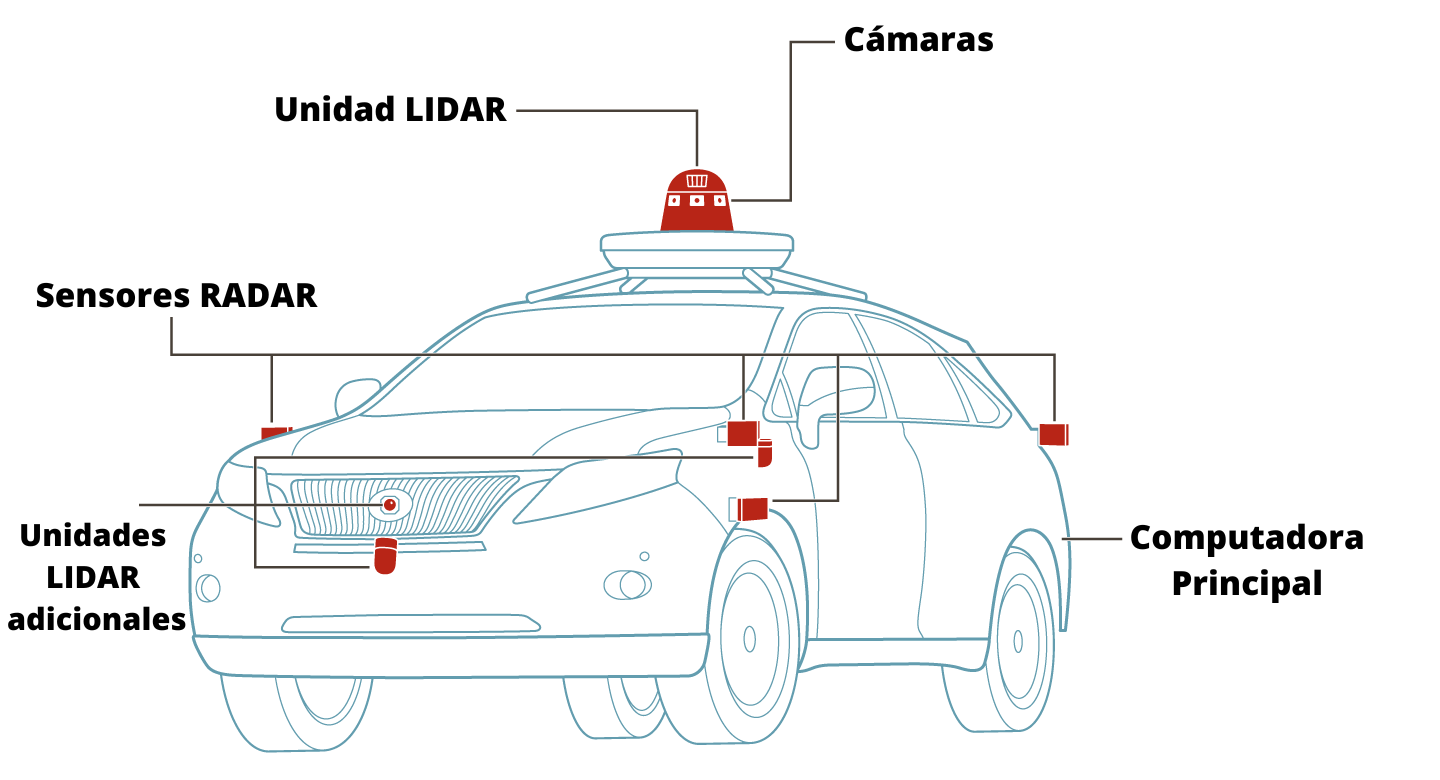
\includegraphics[width=0.7\textwidth]{Figures/Figures_Cap02/self_driving_car.png}
    \caption{Hardware dedicado a vehículos autónomos.}
    \textit{Nota}. Adaptada de \textit{Software Engineering Daily}, 2018 \cite{SoftwareEngineeringDaily}.
    \label{fig:self_driving_car}
\end{figure}

\subsection{Niveles de autonomía} \label{sub:niveles_de_autonomía}

Conducir un vehículo requiere ejecutar gran variedad de acciones y toma de decisiones ya sea si el vehículo se encuentra en movimiento constante o bien, estático en una situación de tráfico. El acto de conducir se puede clasificar en tres diferentes tipos de esfuerzo que realiza el conductor: estratégico, táctico y operativo\cite{michon1985critical}. Los niveles de autonomía de un vehículo motorizado sin conductor se refieren al nivel de ayuda que provee el sistema de automatización con el que está instrumentado. Es decir, el nivel de autonomía es otorgado según el grado de asistencia que se ofrece en la tarea de conducción dinámica.

El término Tarea de Conducción Dinámica o DDT (\textit{Dynamic Driving Task}) por sus siglas en inglés es el concepto que se atribuye a la suma de esfuerzos o funciones tácticas y operativas ejecutadas en tiempo real necesarias para un vehículo en carretera. Otras subtareas como la selección de destinos, programación de viajes y puntos de referencia están excluidas del concepto de DDT porque pertenecen al grupo de funciones estratégicas. Los esfuerzos operativos y tácticos son complementarios, en conjunto resultan como la acción de operar un vehículo\cite{sae2021surface}. De acuerdo con la clasificación de Michon en 1985, el esfuerzo estratégico implica la planificación del viaje, decidir cuándo y dónde ir, cómo viajar, además de elegir la mejor ruta. El esfuerzo táctico incluye técnicas de maniobra durante el trayecto del viaje, esto incluye la toma de decisiones de cómo y cuándo se puede rebasar a otro vehículo, cambiar de carril, mantener velocidad adecuada, revisión de retrovisores laterales y superiores. La última categoría es el esfuerzo operativo que hace referencia a aquellas acciones consideradas innatas o constantes, como es realizar pequeñas correcciones del ángulo de dirección con el volante para mantener el vehículo estable, frenar y acelerar para evitar obstáculos repentinos o eventos peligrosos en el camino\cite{michon1985critical}. 

Ejemplos de funciones operativas y tácticas son:
\begin{enumerate}
\item Operativas
    \begin{itemize}
        \item Control de movimiento lateral por medio de la dirección (\textit{Steering}).
        \item Control de movimiento longitudinal a través de aceleración y desaceleración.
    \end{itemize}
\item Tácticas
    \begin{itemize}
        \item Planificación de maniobras.
        \item Evasión de obstáculos y seguimiento de rutas.
    \end{itemize}
\item Operativas y Tácticas
    \begin{itemize}
        \item Supervisión del ambiente de conducción: detección,  reconocimiento y  clasificación de objetos.
        \item Ejecución de respuesta ante eventos y objetos (OEDR).
    \end{itemize}
\end{enumerate}

La Sociedad de Ingenieros Automotrices (SAE) ha desarrollado un estándar que define la escala de niveles de autonomía. Esta escala determina 6 niveles de autonomía para conducción automática,  desde el nivel 0 (Sin Conducción Automática) hasta el nivel 5 (Conducción Automática Completa)\cite{sae2021surface}. En breve, se enuncian y describen los 6 niveles propuestos por la Sociedad de Ingenieros Automotrices (SAE).

\begin{itemize}
    \item \textbf{Nivel 0: \textit{No Driving Automation}} 
    
    El nivel 0 implica que el conductor es completamente responsable del control de vehículo, es decir, se encarga de las funciones tácticas y operativas. Aunque los vehículos de nivel 0 cuenten con características de seguridad que ayuden a los conductores como: advertencias de colisión y punto ciego, frenado automático de emergencia e incluso cámaras de retroceso,  se clasifican dentro del nivel 0 porque ninguna de estas características actúan durante un periodo prolongado.
    
    \item \textbf{Nivel 1: \textit{Driver Assistance}} 
    
    En el nivel 1 el sistema de conducción automatizado (ADS) toma control del vehículo en situaciones muy específicas. Tal es el caso de control de movimiento lateral y longitudinal, pero no ambas simultáneamente. Esto quiere decir que se mantiene la expectativa de que el conductor realice el resto de la DDT. Un ejemplo es el sistema ACC (\textit{Adaptative Cruise Speed}) que controla la aceleración y el frenado, generalmente en conducciones largas sobre carretera.
    
    \item \textbf{Nivel 2: \textit{Partial Driving Automation}} 
    
    Este nivel de autonomía presenta mejoras en el reconocimiento del entorno y permite al vehículo realizar acciones más complejas. En el caso de control longitudinal para aceleración y frenado, para control lateral ayuda en la corrección de dirección.
    
    De manera general, el nivel 2 provee ayuda por parte del sistema de conducción automatizado (ADS) para cumplir un porcentaje de la tarea de ejecución de respuesta ante eventos y objetos para completar acciones de control en movimiento lateral y longitudinal con asistencia limitada. Existen eventos ante los cuales el sistema no es capaz de responder y por lo tanto, el conductor debe de supervisar el desempeño de la asistencia proporcionada con el  propósito de completar la conducción dinámica (DDT).
    
    \item \textbf{Nivel 3: \textit{Conditional Driving Automation}} 
    
    El nivel 3 es considerado el punto de entrada a la conducción autónoma, pues en situaciones muy específicas con cierto tipo de carreteras y condiciones climáticas adecuadas el conductor comienza a desconectarse del acto de conducir.  
    
    El desempeño por parte del sistema de conducción automatizado es considerablemente mejor, pues toma el control de todas las acciones que permiten completar la tarea de conducción dinámica (DDT). En este nivel aún se mantiene la expectativa de que el conductor este listo ante las solicitudes que pueda requerir el ADS para retomar el control del vehículo en cualquier momento. Un ADS de este nivel permite completar un conducción dinámica en condiciones específicas, por ejemplo en autopistas con velocidad moderada y manejo de frenos. En situaciones de tráfico intermitente el vehículo envía alertas al conductor para que retome el control.
    
    \item \textbf{Nivel 4: \textit{High Driving Automation}} 
    
    En este nivel el sistema de conducción automatizado es completamente capaz de vigilar el entorno de conducción y ejecutar funciones tácticas y operativas. El vehículo también cuenta con la capacidad de alertar al conductor si es que los límites operativos se sobrepasan, en caso de no encontrar respuesta por parte del conductor el vehículo debe asegurarse automáticamente. En otras palabras, un usuario dentro de un vehículo adaptado con características de nivel 4 es un pasajero que no necesita responder ante fallas del sistema.
    
    El cumplimiento de condiciones de riesgo mínimo en adición con la capacidad de recuperación automática resultan ser la principal diferencia que ofrece el ADS  de nivel 4 frente a uno de nivel 3. Vehículos adaptados con condiciones de nivel 4 son capaces de seguir una ruta predeterminada dentro de regiones geográficas limitadas; por ejemplo: circuitos cerrados, campus escolar o una base militar.
    
    %Un ADS diseñado para el nivel 4 está capacitado para cumplir conducción dinámica hacia adelante y hacia atrás, además de lograr una conducción con riesgo mínimo en caso de que el usuario no pueda retomar el control. 
    
    \item \textbf{Nivel 5: \textit{Full Driving Automation}} 
    
    Los vehículos adaptados a un nivel 5 de autonomía son completamente independientes, es decir, el usuario no necesita supervisar el sistema de conducción automatizado. Esto significa que el ADS puede controlar el vehículo dentro de cualquier carretera en cualquier lugar del mundo bajo las mismas condiciones en las que un humano lo pueda hacer.
    
    Esto quiere decir que no existen restricciones climáticas, geográficas o de horario donde pueda operar. Sin embargo, esto no significa que un vehículo del nivel 5 pueda actuar en situaciones donde resulte imposible la tarea de conducción dinámica incluso para los humanos; por ejemplo en tormentas de nieve, derrumbes o inundaciones. En tales casos el ADS debe de lograr una condición de riesgo mínimo, deteniéndose o esperando a que las condiciones cambien. Un vehículo en este nivel puede ser programado con un punto de inicio y un punto de destino siendo capaz de cubrir el trayecto completo en vías públicas independientemente de las condiciones de tráfico, carretera y o clima.
\end{itemize}


%De manera mas concisa se pueden expresar las acciones de manejo que ejecuta el conductor y el sistema de conducción automatizado según el nivel en el que se encuentre.

A partir del nivel 0 y hasta el nivel 3 se entiende que el conductor tiene mayor grado de responsabilidad sobre el manejo del vehículo. El conductor debe de supervisar constantemente las funciones de apoyo con las que cuente el vehículo, según el nivel. Sin embargo, debe de mantenerse atento para frenar, acelerar y dirigir según sea necesario. Un sistema de conducción automatizado (ADS) de estos niveles cuenta con características que permiten proporcionar asistencia y advertencias momentáneas en el caso del nivel 0 por medio de frenado de emergencia automático (AEB)  y advertencia de punto ciego. En los niveles 2 y 3 existen características que ayudan en acciones de control lateral y longitudinal del vehículo como: sistemas ACC y centrado de carril \cite{sae2021surface}.

Los niveles 3, 4 y 5 brindan un mayor grado de asistencia y en consecuencia producen una disminución en las tareas que debe desempeñar el conductor. Para el caso de los niveles 3 y 4 la conducción autónoma es limitada y restringida, el usuario solo retoma el control del vehículo si el sistema de conducción lo solicita. El nivel 5 de autonomía permite navegación de manera completa en cualquier lugar y sin restricciones, el ADS de este sistema esta conformado por una combinación y mejora de cada uno de los componentes usados en niveles inferiores\cite{sae2021surface}.

%en el nivel 5 no se requiere que el conductor se haga cargo de la unidad. 

%La conducción autónoma es limitada y restringida en los niveles 3 y 4, esto se logra por medio de una mayor percepción del ambiente de conducción, en estos dos casos no es necesaria la presencia del conductor al frente del volante, solo si es solicitado por el ADS. 

\subsection{Nivel de autonomía esperado en este trabajo} \label{sub:nivel_de_autonomía_esperado_en_este_trabajo}

En este trabajo se pretende alcanzar un nivel 4 de autonomía, con el fin de lograr este nivel se planea instrumentar un vehículo(simulado en 3D) con sensores que le permitan percibir el ambiente de conducción. LIDAR, cámaras RGB y GPS ayudarán en la estimación de objetos para resolver acciones de rebase y seguimiento de carriles.

También se buscan desarrollar las leyes de control correspondientes para el desempeño de tareas operativas y tácticas de conducción dinámica (DDT). Es considerado como nivel 4 por las características que posee el sistema de conducción automatizada (ADS), además de que la intervención humana es casi nula, pues al ser un ambiente simulado no se cuentan con estas características. Funciones estratégicas quedan fuera del alcance de este trabajo.

\subsection{Sensores} \label{sub:sensores}

\begin{itemize}
    \item \textbf{LIDAR}: \textit{Light Detection and Ranging} por sus siglas en inglés es una tecnología óptica utilizada para detección de objetos, es decir, permite medir distancia y otras propiedades de un objeto objetivo que es iluminado por un haz de luz, a menudo se hace por medio de pulsos láser. Luz ultravioleta, visible o infrarroja son ejemplos de luz que puede usar un sensor LIDAR. Objetos no metálicos, rocas, compuestos químicos, sólidos, nubes e incluso moléculas individuales son ejemplos de objetos que puede detectar este sensor \cite{rathod2013autonomous}.
    % El LIDAR esta diseñado para medir información de rango y proporcionarla al usuario. 
    El principio fundamental de el funcionamiento del LIDAR es emitir un pulso de luz hacia el objetivo y por consecuencia activar un circuito interno de temporización. Internamente se calcula el tiempo que le toma al láser llegar al objetivo y regresar al receptor desde el objetivo, este proceso obtiene la distancia a la que se encuentra el objeto objetivo. Sin embargo, la información que se presenta al usuario puede no estar en un rango real debido a diferentes factores externos, por ejemplo; el ruido inherente del ambiente.

    %puede provocar variaciones inesperadas en sensores de baja escala de hasta 10 centímetros en mediciones de rango, estas variaciones resultan ser perjudiciales en aplicaciones de navegación autónoma o en aplicaciones donde se requiera de una precisión con mayor exactitud\cite{cooper2018range}.
    
    \item \textbf{Cámaras RGB}: Uno de los sensores más complejos utilizados en la robótica son las cámaras digitales. Las cámaras digitales son capaces de capturar y almacenar imágenes digitalmente. De este modo, una cámara RGB es capaz de medir la capacidad de luz dentro de un espectro visible, es decir, el mismo espectro que pueden ver los ojos humanos. Mediante un cámara RGB se pueden captar e interpretar la gama de colores que percibimos los humanos. A diferencia de las cámaras en escala de grises, una cámara RGB agrega una capa de pintura sobre la máscara de píxeles, entonces cada píxel solo registra la intensidad de una determinada componente de color \cite{braunl2003embedded}.
    
    \item \textbf{Cámaras Estéreo}: Una cámara estéreo es un tipo de cámara digital que intenta simular la visión humana y cuenta con la capacidad de capturar imágenes tridimensionales. Una cámara estéreo posee dos o más lentes con un sensor de imagen separado para cada lente, la distancia entre lentes es aproximadamente la distancia promedio en los ojos humanos. Su funcionamiento se basa en tomar una imagen por cada sensor en el mismo instante, luego mezclarlas y obtener como resultado un imagen 3D. El uso de cámaras estéreo es amplio en el sector tecnológico con diferentes campos de aplicación como: vehículos autónomos, astronomía, medicina, topografía, entre otros.
    
    \item \textbf{Cámaras RGB-D}: Las cámaras digitales convencionales producen imágenes como una matriz bidimensional. Por lo general, cada píxel tiene valores asociados al rojo, verde y azul, o RGB. Cada atributo va desde 0 hasta 255, por lo que el color negro es una combinación $(0, 0, 0)$ y un rojo brillante puro sería $(255, 0, 0)$. Juntos miles o millones de píxeles crean este tipo de imágenes. Por otro lado, una cámara de profundidad, tiene píxeles con un valor numérico diferente asociado a ellos, este número representa la distancia o profundidad desde la cámara. 
    Existe diferentes métodos para calcular la profundidad, este se elige según la aplicación en turno. Algunas cámaras de profundidad combinan sistemas RGB más un sistema de profundidad y por lo tanto generan píxeles con los cuatro valores mencionados, o RGBD \cite{cameraRGBD}.
    % \footnote{\url{https://www.intelrealsense.com/beginners-guide-to-depth/}}
    
    \item \textbf{Sonares}: El propósito de los sensores sonares es emitir una señal acústica corta con una frecuencia ultrasónica en un rango de $[50, 250]$ kHz, luego, calcula el tiempo desde la emisión hasta que el eco vuelve al sensor. Este tiempo es proporcional al doble de la distancia del objeto más cercano. Si no se recibe ninguna señal de vuelta en un lapso de tiempo, entonces ningún objeto es detectado en la distancia correspondiente \cite{braunl2003embedded}. 
    Durante décadas, los robots móviles han sido instrumentados con diferentes sensores para navegación, debido a esto, los sensores para medir distancias se encuentran entre los más importantes en robótica. A pesar de lo poderoso que son los sonares en detección de objetos, también poseen desventajas, por ejemplo; interferencias y reflejos. La interferencia ocurre cuando se operan varios sensores de sonar a la vez, por otro lado, los reflejos pueden implicar que un obstáculo parezca estar más lejos de lo que en realidad está.
    
    \item \textbf{GPS}: El sistema de posicionamiento global o GPS de sus siglas en inglés es un sistema de navegación que usa satélites, un receptor y algoritmos para sincronizar información de ubicación, velocidad y tiempo. Se compone de tres componentes diferentes, conocidos como segmentos (satélites, control terrestre, equipo de usuario) y trabajan conjuntamente para proporcionar información de ubicación. El conjunto de satélites utilizado por los GPS consta de una constelación con 24 satélites repartidos en 6 planos orbitales alrededor del planeta Tierra. Solo son requeridos tres satélites para producir una ubicación en la superficie terrestre, sin embargo, a menudo se usa un cuarto satélite para validar información de los otros tres. Además, el cuarto satélite permite calcular la altitud de un dispositivo \cite{gps}.
    % \footnote{\url{https://www.geotab.com/blog/what-is-gps/}}

    Actualmente el uso de GPS está presente en la industria de localización, navegación, seguimiento de objetos, creación de mapas del mundo, entretenimiento, vehículos autónomos, seguridad y comunicaciones móviles.

    %Estos tres segmentos son: \textbf{Satélites}: Giran al rededor de la Tierra y transmiten señales de posición y tiempo, \textbf{Control terrestre}: Son estaciones de monitoreo terrestre, estaciones de control y antenas terrestres para seguimiento y control de satélites en el espacio, \textbf{Equipo de usuario}: Son receptores y transmisores GPS como teléfonos inteligentes, dispositivos telemáticos, entre otros.
\end{itemize}

%\textcolor{red}{Comienza por hablar sobre qué es un vehículo sin conductor y qué características tiene. Tal vez menciona un poco de la historia. Sobre definiciones, puedes encontrar información en:  \url{https://core.ac.uk/download/pdf/234677061.pdf} \url{https://link.springer.com/book/10.1007/978-3-662-48847-8}}

%\textcolor{red}{Habla también sobre los niveles de autonomía y da una breve descripción de cada nivel. Enfatiza el nivel que se logrará en este trabajo. \url{https://www.sae.org/standards/content/j3016_202104/} \url{https://ieeexplore.ieee.org/document/7490340}  \url{https://www.sciencedirect.com/science/article/pii/S095741742030628X?casa_token=WTcFlQ-e2BcAAAAA:KSyYhNe1sPvDkBOi1M2HOrrKU_eX9tIiiLX4AAyAJzDQ8ECByLqFc9RDGbMLDwqU99FljAqykWE}}

%\textcolor{red}{Luego habla de lo que se necesita para que un vehículo pueda ser autónomo: \url{http://ieeexplore.ieee.org/document/6179503/} \url{https://ieeexplore.ieee.org/abstract/document/5940562}}

%\textcolor{red}{Luego hablas de los sensores más comunes que se pueden usar para instrumentar un vehículo sin conductor. Aquí hay una posible lista: \url{https://ieeexplore.ieee.org/stamp/stamp.jsp?arnumber=6179503}}
%\textcolor{red}{
%\begin{itemize}
%    \item Lidar: Cap 8 de \url{https://www.taylorfrancis.com/books/mono/10.1201/b22159/introduction-laser-science-engineering-travis-taylor}
%    \item Cámaras RGB: Cap 1 de \url{https://www.pearson.com/us/higher-education/program/Forsyth-Computer-Vision-A-Modern-Approach-2nd-Edition/PGM111082.html}  Sec. 3.9 de \url{https://www.springer.com/gp/book/9783540343196}
%    \item Cámaras estéreo: Cap 1 de \url{https://www.wiley.com/en-us/An+Introduction+to+3D+Computer+Vision+Techniques+and+Algorithms-p-9781119964476}
%    \item Cámaras RGB-D: \url{https://ieeexplore.ieee.org/document/6619001}
%    \item Sonares Sec. 3.6 de \url{https://www.springer.com/gp/book/9783540343196}
%\end{itemize}
%}

\section{Simuladores} \label{sec:simuladores}

El desarrollo de nuevas tecnologías y agentes inteligentes se encuentra en constante crecimiento a nivel mundial y los vehículos autónomos no son la excepción, debido a la creencia de que los vehículos autónomos pueden ayudar e incluso mejorar tareas de conducción dinámica, comodidad y calidad en viajes. Sistemas inteligentes como ACC, LKA, CA, DN ofrecen mayor eficiencia y confianza en condiciones normales de manejo, en situaciones de tráfico mejoran el rendimiento de combustible y mantienen un ambiente seguro.

El creciente interés en el área de  vehículos inteligentes requiere la innovación de más y mejores componentes que instrumenten a un vehículo que pretende ser autónomo. Una gran variedad de sensores, redes de sensores, tecnologías de comunicación, poder de cómputo y controladores requieren de constantes mejoras y actualizaciones en hardware y software\cite{eskandarian2012handbook}.  En este caso los simuladores son un gran aliado en el diseño y testeo de estos componentes.

%Además, el uso de tecnologías de comunicación abre puertas hacia la generación de nuevos productos y servicios que se basan en la comunicación entre vehículos en un sistema de carretera.

\subsection{¿Por qué usar simuladores?} \label{sub:por_qué_usar_ simuladores}

El desarrollo sistemas para agentes inteligentes en vehículos autónomos es un proceso complejo que involucra diferentes componentes tecnológicos, en específico electrónicos y mecánicos que en conjunto resultan ser difíciles y costosos de conseguir en caso de no contar con los recursos necesarios. Esta es la principal razón para considerar el uso de simuladores durante el desarrollo de sistemas dedicados a vehículos autónomos. Los simuladores permiten realizar desarrollos de muy bajo costo en escenarios similares al mundo real. Otra razón de mucho peso es la seguridad y robustez ante fallos, pues al usar un ambiente simulado se tiene mayor margen de maniobra ante situaciones catastróficas que en un ambiente real podrían resultar perjudiciales.

La simulación juega un papel fundamental en la evaluación y validación del desarrollo de sistemas inteligentes. Además, visto desde otro punto de vista los simuladores poseen características que permiten observación de diferentes conductas en situaciones viales para la formulación de nuevas políticas que permitan mejorar la movilidad. Convirtiéndose entonces en una herramienta para investigar escenarios futuros\cite{eskandarian2012handbook}.

\subsection{¿Para qué usar simuladores?} \label{sub:para_qué_usar_simuladores}

Como se mencionó anteriormente, cumplir con las condiciones y elementos necesarios para el desarrollo de sistemas inteligentes en vehículos autónomos está lleno de riesgos, es a largo plazo, costoso y complejo. Es por ello que el uso de simuladores se vuelve esencial en este desarrollo. 

Los simuladores en este caso ayudan a identificar diferentes aspectos para:
\begin{itemize}
    \item Conceptualizar la idea principal con base de nociones teóricos y modelos matemáticos.
    \item Implementar de ideas con tecnologías que permitan describir el comportamiento esperado.
    \item Desarrollar sistemas completos y creación de prototipos.
    \item Desarrollar productos finales con base en prototipos, sin dejar de lado el mantenimiento y actualizaciones.
\end{itemize}

%De esta manera durante la etapa de desarrollo se buscan cubrir diferentes fases con el fin de lograr la tarea final, como en cualquier proyecto de software se busca minimizar un problema de gran escala en problemas más pequeños y específicos.  
En el caso específico de vehículos sin conductor se buscan simulaciones que permitan diseñar entornos semejantes a condiciones de conducción vehicular en el mundo real. Estos simuladores distinguen diferentes tipos de simulación:
\begin{itemize}
    \item \textbf{Simulación de Tráfico:} Pretende una simulación de todos los sistemas relacionados con el tráfico (control y gestión de tráfico), su propósito es estudiar a los actores involucrados en una red de tráfico (vehículos, conductores, sistemas de tráfico) además de impactos directos en la eficiencia y seguridad del tráfico.
    
    \item \textbf{Simulación de aplicaciones y vehículos:} Es una simulación con mayor detalle de tráfico e involucra más unidades vehiculares en una red de tráfico. El objetivo de esta simulación es el desarrollo de aplicaciones y evaluación técnica.
    %los cuales son modelados con alta fidelidad, se incluyen simulaciones de hardware y software en bucle (HiL, SiL).
    
    \item \textbf{Simulación de comunicación:} El desarrollo de aplicaciones y evaluación del rendimiento de comunicación entre aplicaciones es el propósito de esta simulación. La simulación de comunicación se puede presentar en diferentes niveles según las necesidades y capacidad de computo disponibles.
    %La necesidad de simular telecomunicaciones surgió con la llegada de sistemas cooperativos,
    
    \item \textbf{Simulación de conducción:} Quizás la más importante de las simulaciones es la representación de un conductor, algunas de las funciones no son completamente inteligentes sino que resulta en una cooperación entre conductor y sistema. El objetivo de esta simulación es evaluar el comportamiento de un conductor y el efecto que tiene sobre alguna función específica.
\end{itemize}

Cada ambiente de simulación tiene sus propias necesidades para modelar y describir la dinámica de los actores presentes. Para simular funciones inteligentes en vehículos se requiere de modelos que describan la dinámica del vehículo, sensores, actuadores, conductores, rendimiento de comunicaciones y unidades de carretera. Según las necesidades, en algunos casos los modelos pueden ser reemplazados por simuladores dedicados, como el caso de telecomunicaciones a gran escala donde son manejadas por medio de  modelos estadísticos\cite{eskandarian2012handbook}.

Claramente se puede afirmar que la coherencia entre cada una de las fases de desarrollo de sistemas inteligentes en vehículos es vital con el fin de salvaguardar la portabilidad de resultados. De esta manera se obtiene un marco de trabajo que permite una simulación con diferentes niveles de detalle desde modelos de controladores hasta modelos detallados de sensores y actuadores que al final resultan en procedimientos avanzados de prueba en cada paso de simulación.

\subsection{Motores de físicas, ODE y otros} \label{sub:motores_de_físicas_ODE_y_otros}

Un motor de físicas es un software con la capacidad de realizar simulaciones de comportamientos físicos como: cinemática, dinámica de cuerpos rígidos y blandos, elasticidad, movimiento de fluidos, colisiones. Realizan las operaciones correspondientes para estos comportamientos físicos. Además, manejan los comportamientos de manera independiente del entorno, es decir, reusan código para diferentes situaciones por medio de parámetros. Existe un clasificación para los motores de físicas de acuerdo con la capacidad de procesamiento que requieran: simulación en tiempo real y los de simulación de alta precisión. Las simulaciones de alta precisión requieren de mucha capacidad de computo y generalmente son utilizados con fines científicos, por otro lado las simulaciones en tiempo real se centran más en el campo de los videojuegos.

\textbf{ODE} (\textit{Open Dynamics Engine}) es una biblioteca de gráficos profesional desarrollada en C y C++ y de alto rendimiento para simular dinámicas de cuerpos rígidos. Posee funciones estables, maduras, fáciles de usar y también añade detección de colisiones con fricción. ODE es útil en simulaciones de vehículos, objetos en entornos de realidad virtual y criaturas virtuales. Este motor prioriza la velocidad y estabilidad dejando de lado la precisión física, esto lo hace robusto y confiable pero también poco preciso respecto a otros motores en el mercado. Sin embargo, cuenta con la capacidad de personalizar el entorno incluso durante la simulación \cite{ode}.
% \footnote{\url{https://www.ode.org/}}

Actualmente es utilizado en la industria de videojuegos de ordenador, creación de modelos 3D y herramientas de simulación. Otros motores de físicas importantes para simulaciones en tiempo real y de alta precisión son:
\begin{itemize}
    \item \textbf{Tiempo real:} PhysX, Vortex, Havoc, SOFA, Box2D.
    \item \textbf{Alta precisión:} VisSim
\end{itemize}

\subsection{Bibliotecas para gráficos, OGRE, OpenGL y otros} \label{sub:bibliotecas_para_gráficos_OGRE_OpenGL_y_otros}

Una biblioteca de gráficos es un conjunto de programas enfocados a representar gráficos de computadora en un monitor. Puramente esto se puede realizar ejecutando software directamente en el CPU, o siendo acelerado a través de hardware como en el caso de las GPU. Al emplear este tipo de funciones, un programa ensambla una imagen y posteriormente la envía al monitor. Esto libera al programador de implementar funciones de bajo nivel y concentrarse en especificaciones más concretas de la aplicación. Las bibliotecas de gráficos son utilizadas principalmente en el sector de videojuegos y simulaciones.

\begin{enumerate}
    \item \textbf{OpenGL:} OpenGL es una biblioteca de gráficos para renderizado. En el momento de renderizar OpenGL solo ve una esfera formada por triángulos y un estado de representación. La forma de usar OpenGL es dibujar todo lo que necesita dibujar, luego mostrar una imagen a través de un comando de intercambio de búfer que es independiente de la plataforma. Para actualizar una imagen, se deben dibujar de nuevo todos los componentes, incluso si solo se necesita actualizar una parte del imagen. Para animar objetos en la pantalla es necesario crear un bucle que borre y vuelva a dibujar constantemente en la pantalla.
    Una de las ventajas de OpenGL es ser multiplataforma y permite a los desarrolladores crear aplicaciones de software gráfico atractivas y de alto rendimiento, principalmente en mercados como CAD, entretenimiento, desarrollo de videojuegos, medicina, realidad virtual, fabricación e investigación científica \cite{opengl}.
    % \footnote{\url{https://www.opengl.org/}}
    
    \item \textbf{OGRE:} \textit{Object-Oriented Graphics Rendering Engine} por sus siglas en inglés es un motor de renderizado 3D de software libre, orientado a escenas y escrito en C++.  Las bibliotecas de OGRE evitan la dificultad de utilizar capas inferiores de bibliotecas gráficas como OpenGl y Direct3D, pues provee una interfaz basada en objetos del mundo y otras clases de alto nivel. Específicamente fue diseñado para que a los desarrolladores les resulte más sencillo e intuitivo la producción de aplicaciones gráficas 3D. OGRE actualmente es multiplataforma, y su principal propósito es dar una solución general al renderizado de gráficos con soporte para físicas y audio \cite{ogre}.
    % \footnote{\url{https://www.ogre3d.org/}}
\end{enumerate}

\subsection{Gazebo y sus características} \label{sub:gazebo_y_sus_ características}

Gazebo es un software 3D de código abierto para simulación de robots con modelado de diferentes componentes y entornos, se incluyen texturas de gran calidad, iluminación y sombras. También, ofrece amplía variedad de sensores y actuadores típicos de robótica así como una simulación eficiente de poblaciones de robots en entornos complejos de interiores y exteriores. Gazebo integra OpenGL para gráficos de alta calidad e interfaces gráficas programáticas convenientes y utiliza un motor de físicas robusto, en este caso ODE.

Características destacadas de Gazebo:
\begin{itemize}
    \item Modelos de Robots predefinidos y opciones para crear estilos propios.
    \item Sensores y actuadores con la característica de añadir ruido y obtener simulaciones más reales.
    \item Control e introspección de las simulaciones a través de línea de comandos.
    \item Gráficos 3D avanzados y acceso a múltiples motores de físicas de alto rendimiento como: ODE, Bullet, Simbody y DART.
    \item Simulación en la nube.
    \item Comunidad ampliamente activa.
\end{itemize}

\subsection{Webots y sus características} \label{sub:webots_y_sus_características}

Webots es un software de escritorio de código abierto utilizado en simulación de robots. Provee un completo entorno para modelado, programación y simulación de robots. Es ampliamente usado en campos de educación e investigación además de ambientes industriales. Webots permite crear una gran variedad de simulaciones para diferentes enfoques como: robots de dos ruedas, brazos industriales, robots modulares, vehículos autónomos y aeroespaciales e incluso drones voladores \cite{Webots}.

Los aspectos que hacen de Webots un simulador flexible y robusto son:
\begin{itemize}
    \item Motor de físicas ODE y OpenGL como motor de renderizado.
    \item Es miltiplataforma y disponible para sistemas operativos Linux, Windows y macOS.
    \item Programación de robots en diferentes lenguajes de programación: C, C++, Python, Java, MATLAB e integración con la plataforma ROS.
    \item Robusto, determinista y bien documentado.
    \item Amplía variedad de robots, sensores, actuadores, objetos y materiales.
\end{itemize}


%\textcolor{red}{Por qué y para qué usar simuladores: Cap 7 de \url{https://link.springer.com/referencework/10.1007\%2F978-0-85729-085-4}}
%\textcolor{red}{
%\begin{itemize}
%\item Motores de físicas, ODE y otros
%\item Bibliotecas para gráficos, OGRE, OpenGL y otros.
%\item Gazebo y sus características.
%\item Webots y sus características
%\end{itemize}
%}

\section{Conceptos básicos de visión artificial} \label{sec:conceptos_básicos_de_visión_artificial}

\subsection{Modelo de cámara \textit{pinhole}} \label{sub:modelo_de_cámara_pinhole}
 
 El modelo de cámara \textit{pinhole} permite describir la relación matemática que existe entre las coordenadas de un punto con tres dimensiones y su proyección en el plano de imagen, la apertura de la cámara es descrita por un punto infinitesimal-mente pequeño y no utiliza ningún tipo de lente para enfocar luz \cite{forsyth2011computer}. 
 
 Una cámara \textit{pinhole} es la más simple, no tiene lente y solo cuenta con una y muy pequeña apertura, de ahí deriva su nombre, \textit{pinhole}. Esta cámara puede ser vista como una caja a prueba de luz con un pequeño orificio en alguno de sus lados, siendo este orificio la única entrada de luz. En cuanto la luz de una imagen atraviese el orificio se forma una imagen invertida respecto a la original en el lado opuesto de la caja, ver \ref{fig:pinhole_camera}. A menudo, el modelo \textit{pinhole} es utilizado para describir el cómo una cámara representa un escena en tres dimensiones.
%  \footnote{\url{https://www.vision.uji.es}}
 \begin{figure}
    \centering
    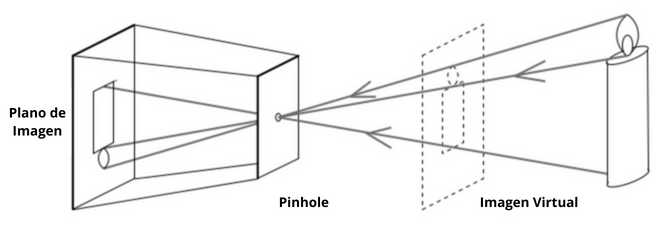
\includegraphics[width=0.6\textwidth]{Figures/Figures_Cap02/pinhole_camera.png}
    \caption{Modelo de cámara \textit{pinhole}.}
    \textit{Nota}. Adaptada de \textit{Computer Vision Group}, 2010 \cite{ComputerVisionGroup}.
    \label{fig:pinhole_camera}
\end{figure}

\subsection{Espacios de Color} \label{sub:espacios_de_color}

La idea de estandarizar el concepto de color surge debido a que los nombres de los colores son insuficientes para toda la gama de combinaciones posibles, otro inconveniente es que un porcentaje de la población solo conoce algunos nombres de colores, y en muchas ocasiones asocian un solo nombre a una gran variedad de un color en específico. 

Se puede entender que los espacios de color o también llamados modelos de color son formas que indican la manera en que un color está definido, permiten aprovechar y analizar toda la información presente dentro de una imagen. Las leyes de Grassman significan que las mezclas de luces de colores se mezclan linealmente, es decir, son una aproximación precisa y lineal\cite{forsyth2011computer}.

Cuando los colores se mezclan linealmente se puede construir un algoritmo sencillo para determinar qué pesos de los primarios se deben de usar para conseguir el color base. Dado que la coincidencia del color es lineal, la combinación de los primarios resulta en una suma ponderada de fuentes de longitud de onda única que es afectada por los pesos específicos de coincidencia. Para cualquier conjunto de primarios (P1, P2, P3) se puede obtener un conjunto de funciones de combinación de colores mediante experimentación\cite{forsyth2011computer}. La Comisión Internacional de la Iluminación CIE (\textit{Commission Internationale d’ eclairage}) ha estandarizado una variedad de sistemas para espacios de color lineales y no lineales.

%Una descripción precisa de colores y estandarizada es un tema de mucha importancia en el sector industrial y tecnológico, pues la mayoría de los fabricantes e investigadores buscan que el mayor porcentaje de los productos tengan el mismo color o al menos sean lo más parecido posible. De esta manera surge la idea de estandarizar el concepto de color, debido a que los nombres de los colores resultan insuficientes para toda la gama de combinaciones posibles, otro inconveniente es que un gran porcentaje de la población conoce solo algunos nombres de colores, y en muchas de las ocasiones asocian un solo nombre a una gran variedad de un color en específico.

%Existe un mecanismo practico y sencillo que permite realizar un emparejamiento de color, tomando como base una combinación de diferentes pesos de los colores primarios hasta empatar el color deseado. Este enfoque también se puede extender para hacer una representación de colores de una superficie si se usa una luz para iluminar la superficie. Este experimento para realizar emparejamiento de colores resulta práctico y en general es el proceso que usan las tiendas de pintura para obtener un color específico con base en combinaciones de pesos de los primarios. Las leyes de Grassman significan que las mezclas de luces de colores se mezclan linealmente, es decir, el emparejamiento es una aproximación precisa y lineal\cite{forsyth2011computer}.

\begin{itemize}
    \item \textbf{Espacios de Color Lineales:}
        \begin{itemize}
            \item \textbf{CIE XYZ:} Creado por la CIE en 1931, las funciones de combinación de color fueron diseñadas para que el resultado obtenido sea positivo en todas partes, es decir, las coordenadas de luz real fueran siempre positivas.
            \item \textbf{RGB:} Es un espacio que utiliza formalmente primarios de una sola onda (R = 645.16nm, G = 526.32nm , B = 444.44nm ). Los colores en este espacio de color se representan mediante un cubo unitario, donde los bordes del cubo son los pesos específicos de las componentes R, G y B.
            \item \textbf{\textit{Opponent Color}:} Es un espacio derivado de RGB que busca tres sistemas de color debido a que existe evidencia acerca de que los primates responden a tres sistemas de color. El más alto responde a la intensidad (Comparaciones claras y obscuras), el segundo compara entre amarillo y azul, el sistema final compara en entre rojo y azul.
\end{itemize}
    \item \textbf{Espacios de Color No Lineales:}
    Un espacio lineal no necesariamente codifica propiedades comunes e importantes en aplicaciones reales. Se excluyen propiedades como tonalidad, saturación y brillo que hacen referencia al cambio de pasar de rojo a verde, de rojo a rosa y de negro a blanco respectivamente. Otra dificultad de los espacios de color lineales es dejar de lado las intuiciones humanas sobre la topología de colores, donde los tonos forman un círculo (Rojo, Naranja, Amarillo, Verde, Cyan, Azul, Morado, Rojo). Esto significa que ninguna coordenada de color en un espacio lineal puede modelar la propiedad de tono\cite{forsyth2011computer}. 

    El espacio HSV( Hue, Saturation, Value), matíz, saturación y valor por sus siglas en inglés es un espacio que basado en RGB y usa una función no lineal para representar las propiedades de tonalidad, saturación y brillo.
    %Por esta razón surge la necesidad de contar con nuevos modelos de color que permitan representar tales propiedades.
\end{itemize}

%En otras palabras, existe una gran cantidad de espacios de color lineales y no lineales que cuentan con características específicas. Sin embargo, la cuestión importante para poder diferenciarlos no es en que sistema de coordenadas se mide el color, sino como se cuenta la diferencia, es decir, la diferencia que existe al momento de buscar reproducir color.

\subsection{Imágenes RGB y su representación en memoria} \label{sub:imágenes_RGB_y_su_representación_en_memoria}
\begin{figure}[h]
    \centering
    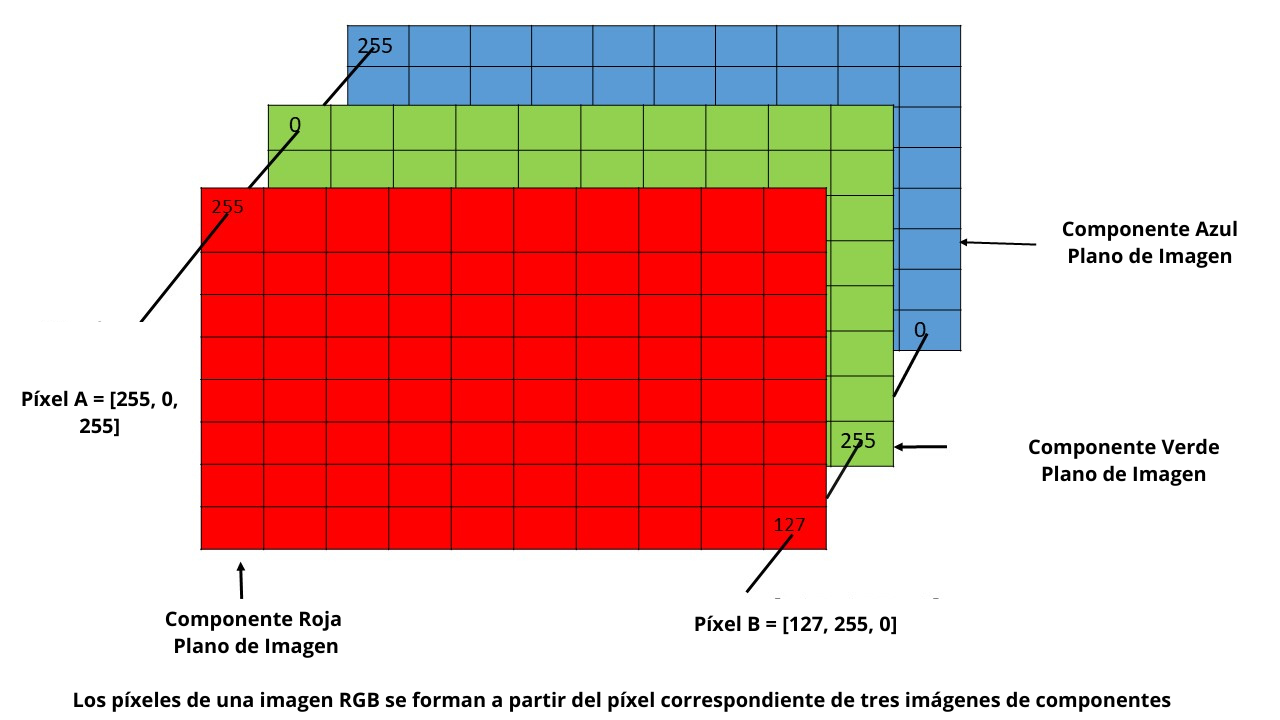
\includegraphics[width=0.75\textwidth]{Figures/Figures_Cap02/rgb_pixels.png}
    \caption{Representación de una Imagen en el espacio RGB.}
    \textit{Nota}. Adaptada de \textit{RGB image representation}, 2018 \cite{RGBImageRepresentation}.
    \label{fig:rgb_pixels}
\end{figure}

Una imagen RGB se puede expresar como tres imágenes diferentes para cada una de las principales componentes RGB (Rojo, Verde, Azul) apiladas una sobre otra, cuando se introducen en un monitor del tipo RGB se combinan para producir una sola imagen de color compuesta. 
La cantidad de píxeles utilizados para representar cada píxel dentro del modelo RGB se denomina profundidad de píxel. Tomando como ejemplo una imagen RGB en la que cada una de las imágenes componentes es de 8-bits en cada píxel (cada píxel es una tripleta de valores [RGB]) tiene una profundidad de píxel de 24 bits, es decir, 3 planos multiplicados por el número de bits (8 bits en este caso), ver \ref{fig:rgb_pixels}. 
% \footnote{\url{https://www.geeksforgeeks.org/matlab-rgb-image-representation/}}

En la práctica, es común escuchar el término de imagen a todo color para referirse a una imagen con profundidad de 24 bits. El número total de colores posibles en una imagen RGB con una profundidad de 24 bits es de $(2^8)^3 = 16 777 216$, es decir, más de 16 millones de combinaciones posibles. De manera que, en cada uno de los ejes (R, G, B) se puede seleccionar un punto en el rango [0, 255], donde el color negro se encuentra en [0, 0, 0] mientras que el blanco se encuentra en [255, 255, 255]\cite{gonzalez2009digital}, la figura \ref{fig:rgb_cube_colors} muestra esto.
% \footnote{\url{https://stackoverflow.com/questions}}
\begin{figure}[h]
    \centering
    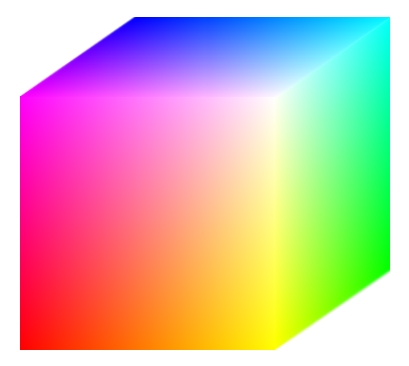
\includegraphics[width=0.3\textwidth]{Figures/Figures_Cap02/rgb_cube_colors.jpg}
    \caption{Cubo de color RGB con profundidad de 24-bits.}
    \textit{Nota}. Tomada de \textit{How to produce RGB cube matrix in python?}, 2014 \cite{stackoverflow}.
    \label{fig:rgb_cube_colors}
\end{figure}

%\textcolor{red}{
%\begin{itemize}
%\item Imágenes RGB y su representación en memoria
%\item Modelo de cámara Pinhole
%\item Espacios de color
%\end{itemize}
%}

\section{Aprendizaje no supervisado} \label{sec:aprendizaje_no_supervisado}

La agrupación de datos en grupos o \textit{clusters} en inglés es una herramienta de la minería de datos con diversos campos de aplicación como biología, seguridad, inteligencia artificial, robótica e incluso búsqueda web. El análisis de grupos es el proceso de distribuir un conjunto de objetos en subconjuntos. Cada subconjunto es conocido como \textit{cluster}, de tal manera que los objetos resultantes dentro de un subconjunto son similares entre sí pero diferentes a los objetos contenidos en otros. Las similitudes y diferencias de los objetos se evalúan en función de las propiedades de los objetos, a menudo, implican medidas de distancia \cite{han2011data}.


\subsection{Agrupamiento (\textit{clustering})}

%El aprendizaje no supervisado es un sinónimo de clustering y se dice que es no supervisado
El agrupamiento es un tipo de aprendizaje no supervisado porque a diferencia del aprendizaje supervisado los datos de entrada no están etiquetados. El agrupamiento es una forma de aprendizaje por observación contrario al aprendizaje mediante ejemplos en el método supervisado. Uno de los retos más grandes del agrupamiento es adaptarse a diferentes tipos y cantidades de datos. Los requerimientos típicos para agrupación en \textit{clusters} dentro de minería de datos son:

\begin{itemize}
    \item \textbf{Escalabilidad:} Necesaria para que algoritmos puedan funcionar de forma aceptable en pequeños y grandes bases de datos.
    
    \item \textbf{Habilidad para tratar con diferentes tipos de atributos:} Muchos algoritmos son diseñados para datos numéricos. Recientemente más y más aplicaciones en el campo de la informática requieren de técnicas de agrupamiento para tipos de datos más complejos como grafos, imágenes y documentos.
    
    \item \textbf{Descubrimiento de \textit{clusters} en forma arbitraria:} Es importante desarrollar algoritmos que puedan detectar \textit{clusters} de forma estándar, diferentes algoritmos determinan \textit{clusters} en base a mediciones de distancia Euclidiana o distancia de Manhattan y centran sus esfuerzos en formar grupos esféricos con tamaño y densidad similares. Sin embargo, un grupo puede tener cualquier forma.
    
    \item \textbf{Habilidad para tratar con datos ruidosos:} Muchos conjuntos de datos reales pueden contener valores atípicos, erróneos o desconocidos. Lecturas de sensores, por ejemplo, a menudo son ruidosas y pueden producir valores incorrectos. Los algoritmos de agrupamiento tienden a ser sensibles al ruido de estas lecturas y pueden generar mala calidad en resultados finales. Por lo tanto, se requiere de métodos robustos ante el ruido. 
    
    \item \textbf{Capacidad para agrupar conjuntos de datos con dimensiones grandes:} Muchos algoritmos de agrupación generan resultados rápidos en conjuntos de datos dimensionalmente pequeños, caso contrarío con lo que sucede con conjuntos más amplíos donde el desempeño de los algoritmos se ve comprometido.
    
    \item \textbf{Interpretabilidad y usabilidad:} Es importante estudiar cual será el campo de aplicación del agrupamiento para realizar una buena elección en el algoritmo a implementar y al final del proceso se obtengan resultados entendibles, usables y con valor para la aplicación.
    
    \item \textbf{Medida de similitud:} Las medidas de similitud juegan un papel importante en el diseño de métodos de agrupamiento. Los métodos basados en distancia a menudo pueden aprovechar técnicas de optimización en el desarrollo, mientras que métodos basados en densidad o continuidad por lo general pueden encontrar grupos con formas arbitrarias.
\end{itemize}

Por lo general, se utiliza el aprendizaje no supervisado para descubrir automáticamente diferentes tipos clases dentro de un conjunto de datos, esta es una clara ventaja del aprendizaje no supervisado frente a otro tipo de aprendizaje porque un \textit{cluster} de objetos puede ser entendido como una clase implícita, pues los elementos de un \textit{cluster} son similares entre si pero diferentes respecto a objetos de otros \textit{clusters} \cite{han2011data}. 

\section{Máquinas de estados finitos} \label{sec:máquinas_de_estados_finitos}

\subsection{Definición} \label{sub:definición}

Las máquinas de estados finitos o FSM (\textit{Finite State Machine}) por sus siglas en inglés son el corazón en la mayoría de los diseños digitales. La idea principal de una FSM es almacenar un conjunto de diferentes estados únicos y realizar transición entre ellos con base en los valores de entrada y el estado actual de la máquina. Una máquina de estados finitos puede ser de dos tipos: Moore y Mealy \cite{wilson2013model}. La primer forma específica que, la salida de la máquina de estados depende puramente de las variables de estado. Por otro lado, en una máquina Mealy la salida puede depender de las variables de estado actuales y valores de entrada a la máquina. El método para describir una FSM es utilizar un diagrama de transición de estados. Este diagrama muestra los estados, salidas y condiciones de transición.

Una alternativa al uso de máquinas de estados finitos es utilizar una técnica llamada Máquina de Estados Algorítmicos (ASM) o carta ASM, esta técnica es útil porque permite separar la ruta de datos y control en un diagrama simple. Una carta ASM es similar a un diagrama de flujo, con acciones y decisiones que pueden ser combinatorias y secuenciales. La diferencia entre FSM Y ASM es la manera gráfica en que se expresan, la forma gráfica de una carta ASM permite definir explícitamente estados, decisiones y resultados, con apariencia similar a un diagrama de flujo. Esto hace que el algoritmo sea más entendible que un diagrama de transición de estados. Una carta ASM tiene tres bloques principales, en \ref{fig:asm_blocks} se ilustran.

\begin{itemize}
    \item \textbf{Estado:} Es representado por una caja rectangular, contiene el valor del estado actual, como un nombre o valor numérico que representa la variable de estado. También puede contener el valor de las salidas según el tipo de máquina de estado (Mealy o Moore).
    \item \textbf{Decisión:}  El bloque de decisión indica diferentes caminos condicionales dependiendo del valor de las variables de entrada. Este bloque es representado en forma de diamante.
    \item \textbf{Salida:} Una salida puede ser condicional o incondicional. Donde; una salida es condicional cuando es precedida por un diamante de decisión (Mealy), por el contrario una salida condicional está presente en un estado sin decisión previa (Moore).
\end{itemize}

\subsection{Formas de implementarlas} \label{sub:formas_de_implementarlas}

Tanto las máquinas de estados finitos (FSM) y las máquinas de estados algorítmicos pueden ser implementadas en diferentes lenguajes de programación, en específico mediante el paradigma de programación imperativa, es decir, la implementación de la máquina debe consistir en una secuencia claramente definida de instrucciones. Las instrucciones se encadenan una detrás de otra para determinar el comportamiento en cada momento y lograr el resultado deseado. Algunos lenguajes que implementan este paradigma son: Python, C, C++, Ensambladores, Ruby, Pascal.
\begin{figure}[h]
    \centering
    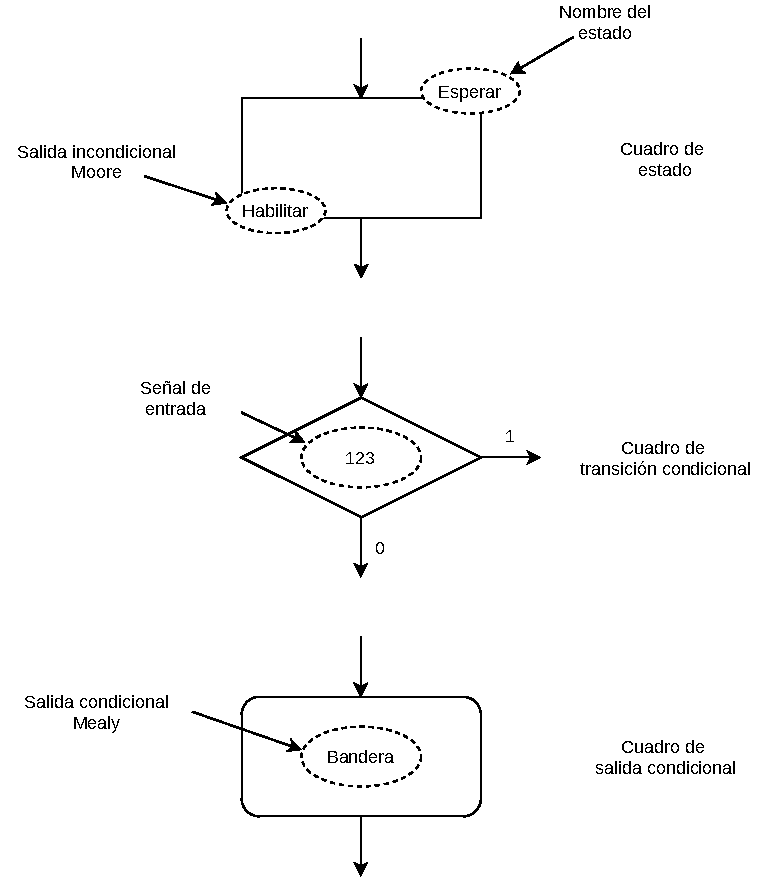
\includegraphics[width=0.5\textwidth]{Figures/Figures_Cap02/asm_chart.pdf}
    \caption{Bloques de una carta ASM.}
    \label{fig:asm_blocks}
\end{figure}


%\textcolor{red}{
%\begin{itemize}
%\item Definición
%\item Formas de implementarlas (memorias y en lenguajes imperativos)
%\end{itemize}
%}

\section{Trabajo relacionado} \label{sec:trabajo_relacionado}

\subsection{Los vehículos Tesla y de Google} \label{sub:los_vehículos_tesla_y_de_google}

\begin{itemize}
    \item \textbf{Tesla:} La compañía Tesla fue fundada en 2003 por un grupo de ingenieros, su objetivo inicial era demostrar que es posible conducir con energía eléctrica y que los vehículos eléctricos pueden ser más rápidos y divertidos de manejar que los vehículos a gasolina. Además, la empresa se enfoca en desarrollar tecnologías que sumen a la conducción autónoma. Tal es el caso de su tecnología Autopilot.
    
    El sistema Autopilot incluye un sofisticado conjunto de cámaras delanteras, traseras, laterales, amplias y estrechas. En adición con una base de red neuronal profunda, el vehículo deconstruye el entorno para incluir mayor nivel de confiabilidad. En la parte de procesamiento, Autopilot añade una capa de hardware con alta velocidad de procesamiento para ejecutar la red neuronal, que es la base de entrenamiento y desarrollo del Autopilot.
    
    Este sistema permite navegar en condiciones viales reales y realizar acciones tediosas durante la conducción como: maniobrar, acelerar y frenar automáticamente dentro del carril. Con su característica Autosteer un Tesla puede navegar en calles estrechas y complejas, con Smart Summon el vehículo puede conducir en entornos y espacios de estacionamiento para efectuar un estacionamiento completamente autónomo. Actualmente las funciones de este sistema requieren una supervisión activa del conductor para no dejar que el vehículo sea completamente autónomo. El uso sin supervisión de un conductor depende de que se logre una confiabilidad superior a las habilidades de conductores humanos, además de demostrarlo con millones de kilómetros recorridos, así como diferentes aprobaciones legales \cite{autopilot}.
    % \footnote{\url{https://www.tesla.com/es_MX/autopilot}}
    
    Tesla no solo produce vehículos totalmente eléctricos y tecnología autónoma, también fabrica productos de almacenamiento y generación de energías limpias que pueden ampliarse de manera ilimitada. 
    % \footnote{\url{https://www.tesla.com/es_MX/about}}
    
    
    
    %En el año 2008 fue lanzado al mercado el Roadster, introdujo tecnología de vanguardia para baterías y sistemas de propulsión eléctrica. Desde entonces Tesla ha desarrollado diferentes modelos de vehículos eléctricos como: el primer sedán 'Model S' \ref{fig:tesla_cars} totalmente eléctrico, años más tarde surgió el 'Model X', como el SUV más rápido, seguro y con mayor capacidad de la historia. Además de vehículos más grandes como camiones y camionetas, el 'Tesla Semi' y 'Cybertruck' respectivamente. \textcolor{red}{Hablar sobre los algoritmos de conducción autónoma y no tanto sobre vehículos eléctricos. }
    
    \item \textbf{Google:}
    Anteriormente conocido como ``Proyecto de vehículo autónomo de Google'' en 2009, Waymo es una empresa de tecnología dedicada a vehículos autónomos, su misión es lograr que pasajeros y objetos lleguen de forma fácil y segura a su destino. Su tecnología busca mejorar el acceso a la movilidad, mientras intenta salvaguardas vidas que se podrían haber perdido en accidentes vehiculares.

    Waymo enfoca sus esfuerzos en el desarrollo de Waymo Driver, su tecnología de conducción autónoma y se divide en dos partes: hardware y software. La parte de hardware incluye un paquete de instrumentación con sistemas lidar, cámaras, radares y una importante plataforma de procesamiento de inteligencia artificial, en conjunto forman una vista de $360^{\circ}$ del ambiente. El software recopila la información de todos los sensores para saber ¿Dónde está?, ¿Qué existe a su alrededor? y ¿Qué debe hacer?. El hardware y software trabaja en conjunto para crear una imagen completa del mundo que rodea al vehículo y navegar de forma segura por las calles \cite{waymo}.
    % \footnote{\url{https://waymo.com/intl/es/faq/}}

    La flota de vehículos de Waymo incluye al Toyota Prius, vehículos deportivos Lexus, un vehículo prototipo (Firefly) y camionetas híbridas Chrysler, ver \ref{fig:waymo_cars}.
\end{itemize}
\begin{figure}[h]
    \centering
    \begin{subfigure}{0.4\textwidth}
         \centering
         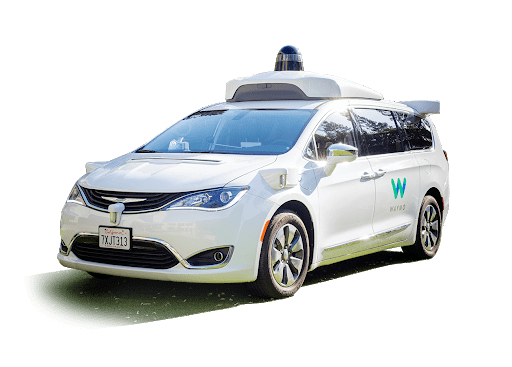
\includegraphics[width=\textwidth]{Figures/Figures_Cap02/waymo_car.png}
         \caption{Vehículo Waymo.}
         \textit{Nota}. Tomada de \textit{Waymo}, 2022 \cite{waymo}.
         \label{fig:waymo_cars}
    \end{subfigure}
    \hfill
    \begin{subfigure}{0.4\textwidth}
         \centering
         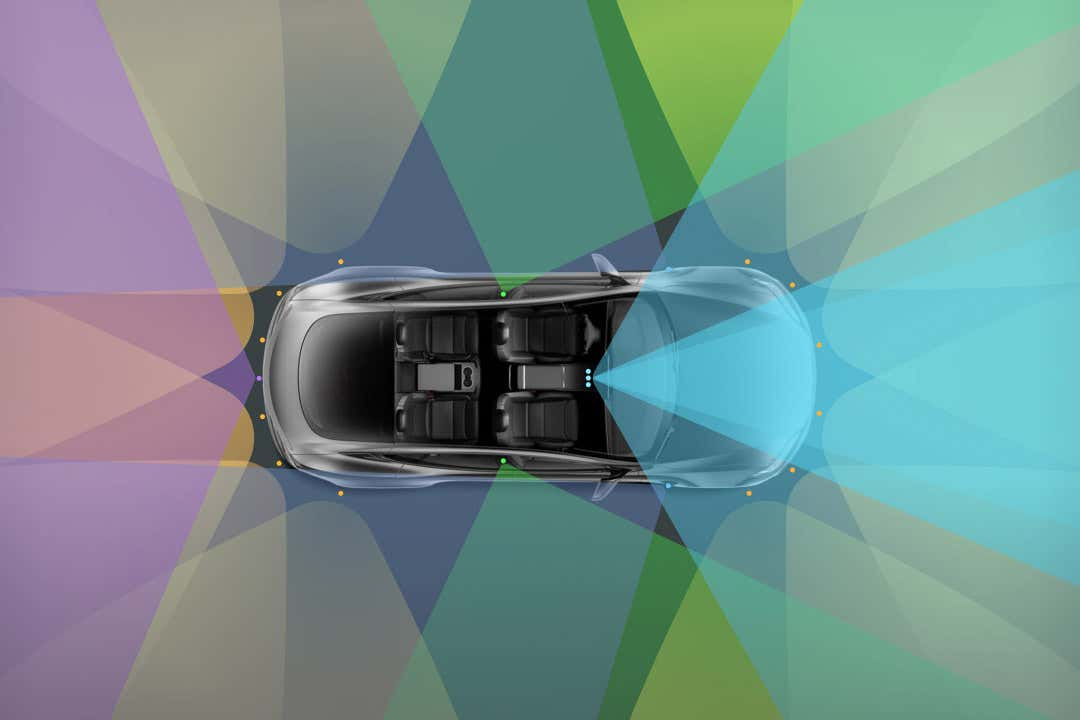
\includegraphics[width=\textwidth]{Figures/Figures_Cap02/tesla_car.jpg}
         \caption{Vehículo Tesla con Autopilot.}
         \textit{Nota}. Tomada de \textit{Autopilot-Tesla}, 2022 \cite{autopilot}.
         \label{fig:tesla_cars}
     \end{subfigure}
    \caption{Vehículos Waymo y Tesla.}
    \label{fig:waymo_tesla_cars}
\end{figure}

\subsection{La categoría AutoModelCar del TMR} \label{sub:la_categoría_autoModelCar_del_TMR}

El Torneo Mexicano de Robótica (TMR) es la competencia de robótica más importante en México. Tiene como principal objetivo motivar e impulsar la investigación y desarrollo de la robótica en busca de un desarrollo integral de nivel internacional. El TMR incluye diferentes categorías de competición con diferentes enfoques \cite{tmr}.
% \footnote{\url{https://www.femexrobotica.org/tmr2022/}}

La categoría AutoModelCar busca incentivar el desarrollo de algoritmos de percepción, planificación y control para vehículos autónomos. Los vehículos no tripulados que participan en esta categoría son modelos a escala 1:10 instrumentados con sensores y actuadores similares a los que tendría un vehículo autónomo en la vida real. Sin embargo, también existe una categoría donde se utilizan simuladores para efectos del vehículo, sensores y actuadores \cite{AutoModelCar}. Esta categoría permite el desarrollo de los mismos algoritmos, además de abrir puertas a la participación a distancia, la figura \ref{fig:tmr_auto_model_car} es una representación de un vehículo a escala utilizado en el TMR en su modalidad presencial. 
% \footnote{\url{https://www.femexrobotica.org/tmr2022/automodelcar/}}
\begin{figure}[h]
    \centering
    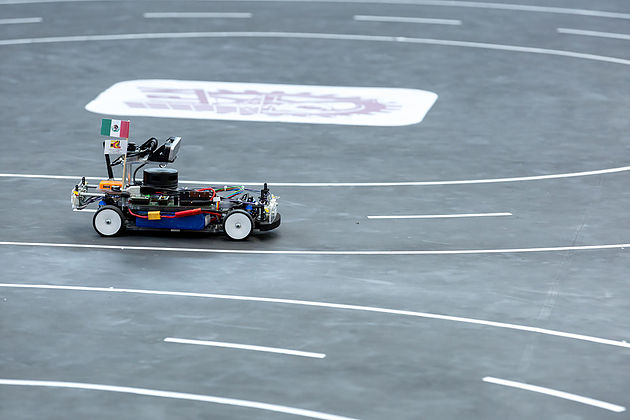
\includegraphics[width=0.5\textwidth]{Figures/Figures_Cap02/automodel_car.jpg}
    \caption{Categoría AutoModelCar del TMR.}
    \textit{Nota}. Tomada de \textit{TMR-AutoModelCar}, 2022 \cite{AutoModelCar}.
    \label{fig:tmr_auto_model_car}
\end{figure}

\subsection{El equipo FUB} \label{sub:el_equipo_FUB}

El trabajo desarrollado por la Universidad Libre de Berlín incluye hardware y software. Cuenta con modelos de vehículos a escala 1:10 y el hardware añade: sensores LIDAR, cámaras RGB con diferentes rangos de visión, puertos USB y adaptadores de red. El software de estos modelos se encuentra sobre la plataforma ROS, este software implementa algoritmos que permiten realizar diferentes tareas de navegación como: detección de líneas de carril, detección de señales de tráfico, control de movimientos, entre otros. Para obtener información más detallada sobre este proyecto visitar \footnote{\url{https://github.com/AutoModelCar/AutoModelCarWiki/wiki}}.






%\textcolor{red}{
%\begin{itemize}
%\item Los vehículos Tesla y de Google
%\item https://github.com/AutoModelCar/AutoModelCarWiki/wiki
%\item La categoría AutoModelCar del TMR
%\item El trabajo hecho en el laboratorio de Biorrobótica
%\end{itemize}
%}

% CONCLUSIONES DEL CAPÍTULO
En este capítulo se presentaron en los conceptos teóricos básicos que serán necesarios a lo largo de este trabajo. Se dio a conocer el término de vehículo autónomo y las características necesarias que requiere para ser considerado como tal, con base en ello se indicó el nivel de autonomía que es pretendido alcanzar al finalizar este proyecto.

En los capítulos siguientes se abordaran de manera específica y detallada muchas de las definiciones aquí mencionadas, también, se expondrán implementaciones de las mismas en aplicaciones para vehículos sin conductor.




\chapter{Simulación con Webots} \label{cap:simulación_con_webots}
% BREVE DESCRIPCIÓN DEL CONTENIDO DE ESTE CAPÍTULO
Webots es el simulador utilizado en el resto de este trabajo para mostrar el funcionamiento de los diferentes algoritmos desarrollados, este capítulo expone sus cualidades. En la sección \ref{sec:conceptos_básicos_del_simulador_Webots}, se describen las principales características que posee, los lenguajes y plataformas compatibles con el software. También, se definen conceptos esenciales para el desarrollo con el simulador como: mundo, controladores y controladores supervisores. La sección \ref{sec:el_formato_open_street_maps} explica la forma de integrar el formato \textit{Open Street Maps} con Webots en la búsqueda de crear escenarios de prueba más realistas. Por otro lado, la sección \ref{sec:el_ambiente_de_simulación} presenta las necesidades requeridas en este proyecto, se listan las características del ambiente simulado y del vehículo de pruebas, a continuación, se muestran los modelos finales del vehículo y escenario de pruebas. La sección \ref{sec:contribuciones_en_el_TMR} da a conocer las contribuciones de este trabajo en el TMR-AutoModelCar 2022.


\section{Conceptos básicos del simulador Webots} \label{sec:conceptos_básicos_del_simulador_Webots}

Webots es un software multiplataforma de código abierto enfocado a simulación de robots móviles, el ambiente de Webots provee un entorno de desarrollo completo que facilita la programación, modelado y simulación de robots de manera profesional. También, le permite al usuario crear entornos virtuales 3D con propiedades físicas importantes en el comportamiento de robots, tal es el caso de propiedades como: masa, coeficiente de fricción, articulaciones, entre otros\cite{Webots}.

En el simulador se pueden encontrar objetos pasivos y activos también llamados robots móviles, estos pueden ser equipados con una gran variedad de sensores y actuadores que contiene el propio simulador, donde destacan: sensores de distancia, sensores láser, motores, cámaras, ruedas, gps, emisores y receptores. Además ofrece al usuario la facilidad de programar de manera individual cada robot creado con el fin de lograr el comportamiento deseado para cada uno. La figura \ref{fig:webots_ui} ilustra la interfaz de usuario de Webots.
\begin{figure}
    \centering
    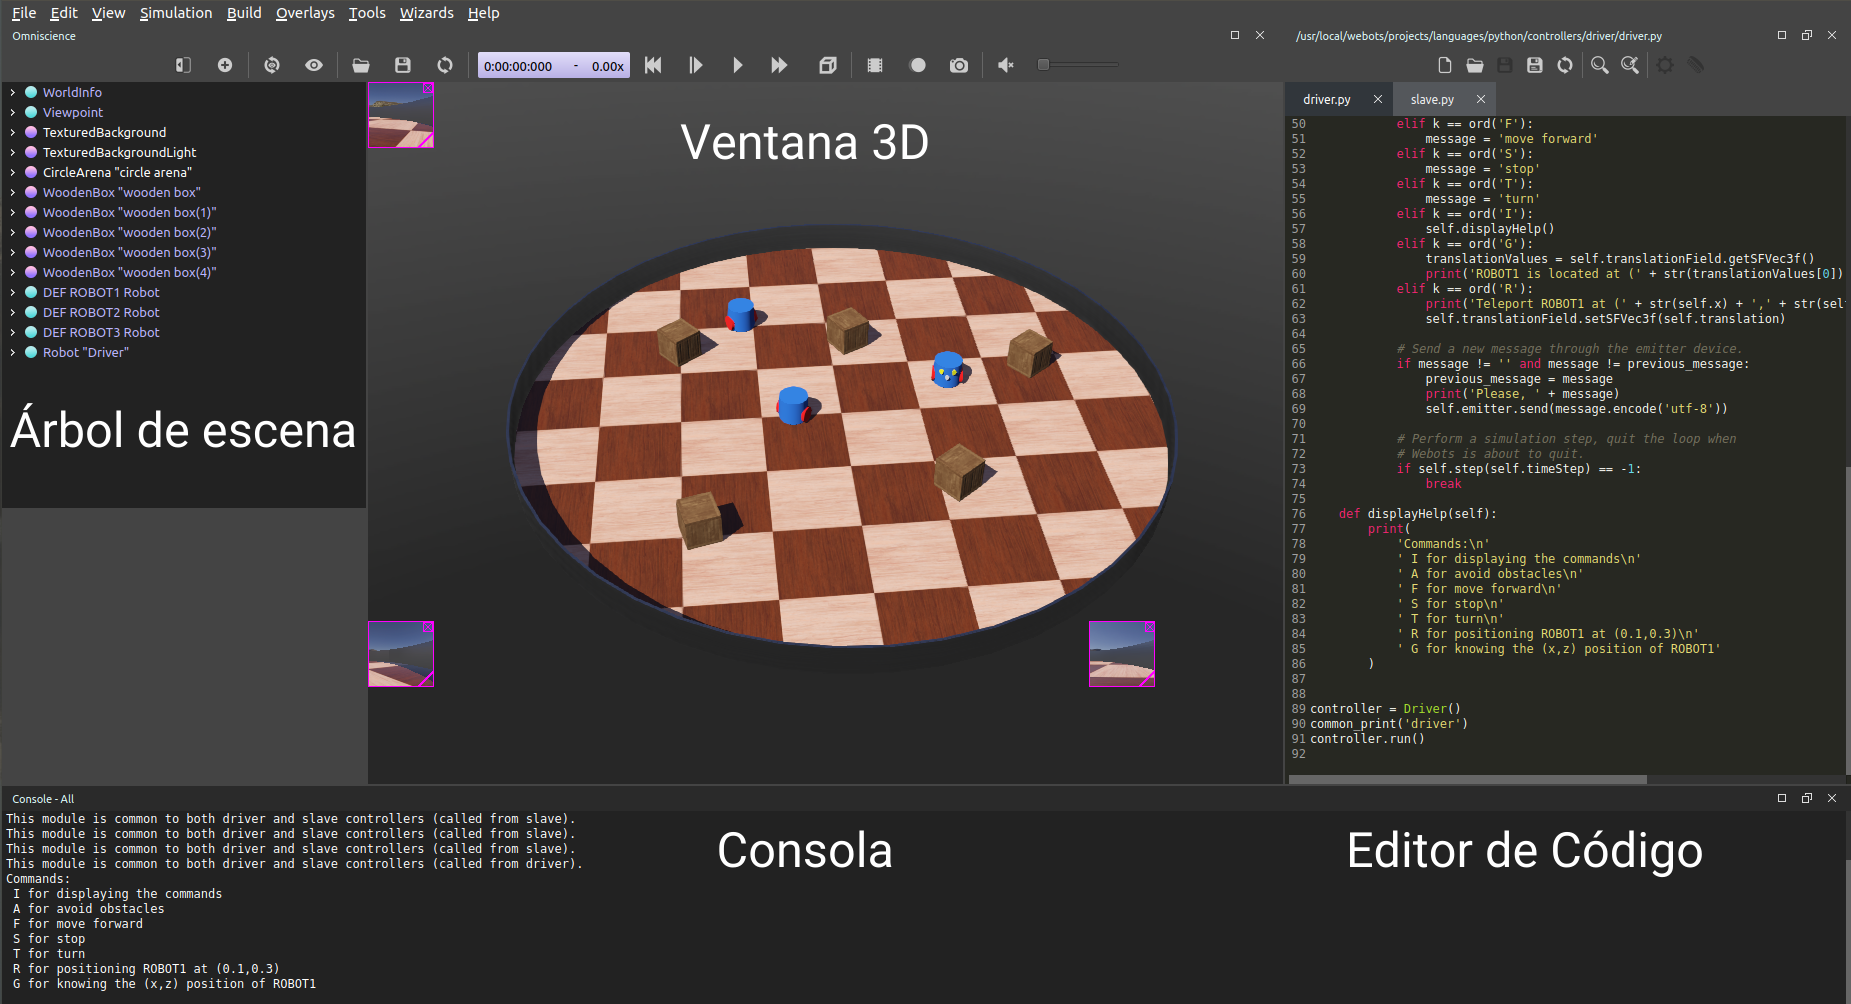
\includegraphics[width=0.5\textwidth]{Figures/Figures_Cap03/WebotsUserInterface.png}
    \caption{Interfaz de Usuario Webots.}
    \label{fig:webots_ui}
\end{figure}

\subsection{Lenguajes y Sistemas Operativos}

Al ser un software de código abierto Webots puede ser utilizado en diferentes plataformas de escritorio como: Windows, Linux y macOS. Para cada una de estas plataformas se encuentra disponible la documentación correspondiente, además existe una comunidad muy activa en cada una de sus variantes. Sin embargo, las distribuciones Linux son las que se mayor ayuda proveen, esto debido a la amplia compatibilidad entre Webots y las diferentes herramientas en el desarrollo de robots móviles. Por otra parte, Webots cuenta con soporte para diferentes lenguajes de programación en la creación de programas controladores, entre los lenguajes soportados se encuentran lenguajes compilados como: C, C++ y Java, también permite el uso de lenguajes interpretados como: Python y MATLAB\cite{Webots}.

\subsection{Controladores, supervisores y mundos} 

Para crear una simulación en Webots son necesarios dos elementos principales: un mundo y uno o varios controladores.

\begin{itemize}
    \item \textbf{Mundo:} En Webots un mundo es el conjunto de elementos que unido al robot forman una escena 3D o abstracción del mundo real con el fin de simular un ambiente real. Un mundo específica la descripción de cada objeto mediante propiedades como: posición, geometría, orientación, apariencia y propiedades físicas (en caso de ser necesarias). Cada objeto definido puede contener a su vez otro objeto diferente\cite{Webots}. En la figura \ref{fig:webots_example}, se observa un mundo de ejemplo creado en Webots. 
    %un mundo es una representación del ambiente mediante la descripción en 3D de las propiedades de el robot y el entorno en el que se encuentra, es decir, 
    
    \item \textbf{Controlador:} Es un programa que permite ejecutar acciones de control para un robot específico en un mundo específico. Dichos controladores pueden ser desarrollados en los diferentes lenguajes de programación soportados(C, C++, Java, Python, MATLAB). Para cada uno de estos lenguajes se provee la documentación necesaria. Una característica importante de los controladores es que un controlador puede ser utilizado por diferentes robots pero un robot solo puede usar un controlador. Al iniciar una simulación Webots lanza los controladores previamente asignados en cada robot, es decir, para cada controlador existe un proceso independiente\cite{Webots}.
    
    \item \textbf{Controlador Supervisor:} Este tipo de controladores son una variante especial de los controladores tradicionales, la principal diferencia entre ellos es que los controladores supervisores tienen acceso a operaciones privilegiadas. Por ejemplo; el control de simulación para mover el robot a una posición aleatoria, realizar una captura de vídeo de la simulación, entre otras. Los supervisores también pueden ser escritos en los lenguajes soportados por Webots\cite{Webots}.
\end{itemize}

\begin{figure}[h]
    \centering
    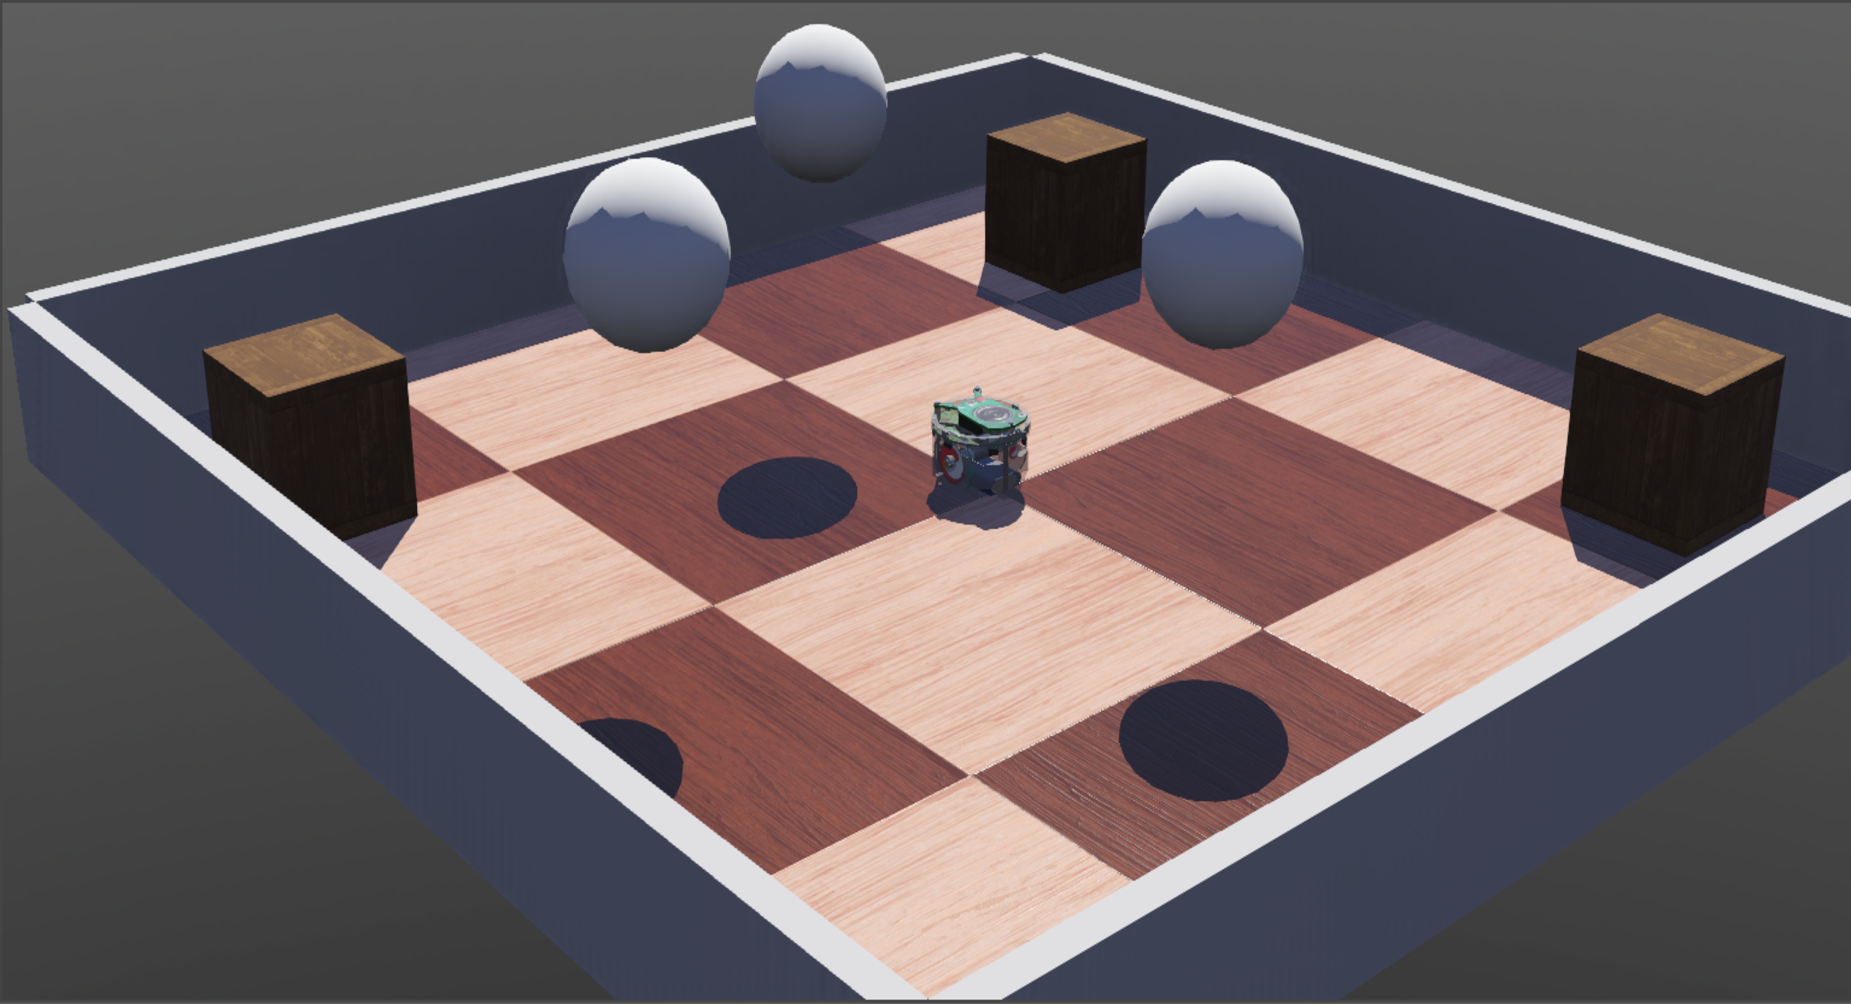
\includegraphics[width=0.5\textwidth]{Figures/Figures_Cap03/WebotsWorldExample.png}
    \caption{Ejemplo de mundo en Webots.}
    \label{fig:webots_example}
\end{figure}

%\textcolor{red}{
%\begin{itemize}
%\item Lenguajes y sistemas operativos soportados
%\item Controladores, mundos y controladores supervisores.
%\end{itemize}
%}

\section{El formato \textit{Open Street Maps}} \label{sec:el_formato_open_street_maps}

\subsection{Características y especificaciones}

El formato \textit{Open Street Maps} es un proyecto de software libre, global y cooperativo para la creación de mapas en base a información geográfica capturada por dispositivos GPS y ortofotografías, al ser un proyecto libre se cuenta con grandes cantidades de información y representación de mapas de casi cualquier sitio del mundo. Con base en el formato \textit{OSM} Webots es capaz de transformar la información del mapa en un ambiente 3D donde los principales objetos son las carreteras, conexiones viales y edificios. Además, mediante la integración de nodos específicos como: vehículos, señales de tránsito, obstáculos y mobiliario urbano se obtiene un ambiente de simulación (mundo 3D) con mayor detalle para el desarrollo de pruebas en conducción autónoma.

\subsection{Como usarlo en Webots}

Con el fin de implementar tareas de vehículos autónomos se requiere de un ambiente de simulación que cuente con las características necesarias y que sean lo más parecidas a un ambiente del mundo real. Para lidiar con este aspecto Webots ofrece una herramienta muy útil, la cual es generar modelos 3D a partir de una sección del mundo real tomada del formato \textit{Open Street Maps}. La manera de integrar OSM con Webots es muy sencilla debido a que desde la instalación inicial del simulador se incluyen las herramientas necesarias. En breve se enuncian los pasos a seguir para crear un escenario 3D inspirado en un mapa real.
\begin{figure}
        \centering
        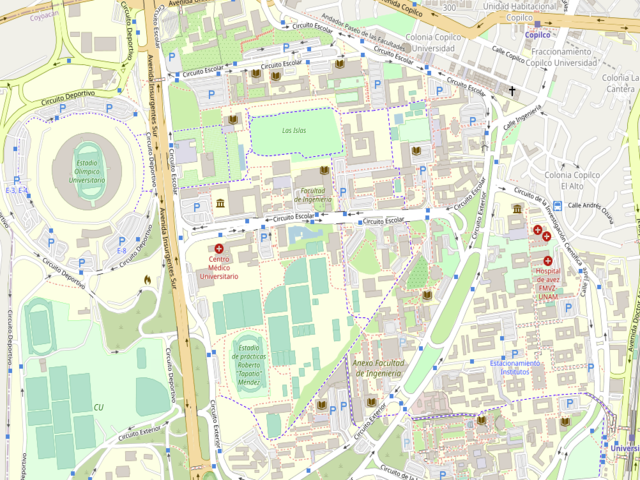
\includegraphics[width=0.5\textwidth]{Figures/Figures_Cap03/cu_osm.png}
        \caption{Sección de mapa obtenida de \textit{Open Street Maps}.}
        \label{fig:cu_osm}
\end{figure}

\begin{enumerate}
    \item Crear un directorio donde se alojará el proyecto.
    \item Obtener y descargar el mapa en formato OSM desde la página oficial de \textit{OpenStreetMap} \ref{fig:cu_osm} para generar el mundo de Webots.  
    %Desde la página web de OpenStreetMap se cuenta con la opciones para buscar y obtener una sección específica del mapa, en se aprecia una sección de mapa en Open Street Maps.
    
    \item Generar el mundo de Webots a partir del mapa obtenido. Webots cuenta con script ``importer.py'' que recibe como parámetro un archivo con extensión ``.osm'' y retorna como salida un archivo con extensión ``.wbt''. Es necesario ejecutar el script ``importer.py'' asignando como entrada el mapa previamente obtenido. Si la operación es exitosa se debe localizar un archivo ``.wbt'' en el directorio creado al inicio. Desde Webots se puede abrir el archivo para su visualización.
    
    \item Entrar a Webots y editar las carreteras, caminos y nombres de los mismos con el fin de eliminar cualquier \textit{bug} producido por ``importer.py'' debido a la complejidad del archivo ``.osm''. En esta etapa se pueden agregar más objetos (autos, árboles, señales, edificios, obstáculos) según sean requeridos. La figura \ref{fig:cu_wbt} muestra el resultado esperado de este proceso.
\end{enumerate}
\begin{figure}[h]
    \centering
    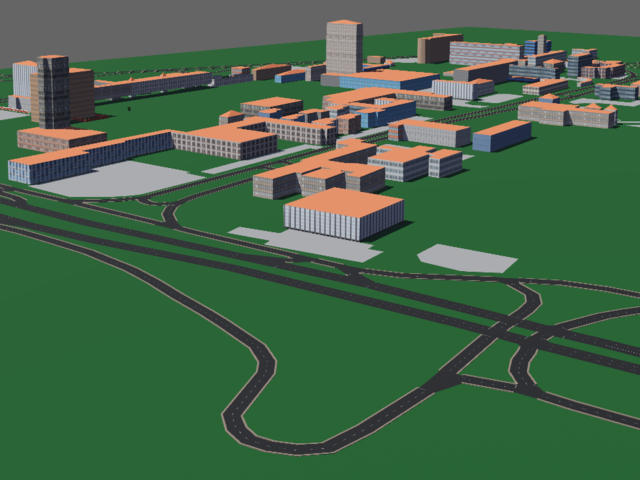
\includegraphics[width=0.45\textwidth]{Figures/Figures_Cap03/cu_wbt.png}
    \caption{Mundo de Webots generado a partir de una sección de mapa en formato ``.osm''.}
    \label{fig:cu_wbt}
\end{figure}


%\textcolor{red}{
%\begin{itemize}
%\item características y especs
%\item Cómo usarlo con Webots
%\end{itemize}
%}

\section{El ambiente de simulación} \label{sec:el_ambiente_de_simulación}

En la búsqueda de modelar comportamientos de vehículos autónomos reales como: detección y seguimiento de carriles, seguimiento de vehículos, detección y evasión de obstáculos tanto estáticos como dinámicos, es de vital importancia tener un escenario los más parecido posible a un ambiente vial cotidiano. Un ambiente vehicular tradicional es aquel que cuenta con automóviles en movimiento y estáticos, señales de tránsito, semáforos, carriles con dirección y espacios definidos. Además de contar con construcciones como edificios, casas, puentes e incluso personas y animales. Cada uno de estos elementos en conjunto forman un ecosistema vial como cualquier otro presente en localidades urbanas.

En este trabajo se pretende modelar un escenario 3D con el simulador Webots que integre las características suficientes para realizar ejercicios de prueba de diferentes comportamientos como:
\begin{itemize}
    \item Detección de Carril
    \item Seguimiento de Carril
    \item Detección de Obstáculos
    \item Evasión de Obstáculos
    \item Seguimiento de vehículos
    \item Acciones de rebase
\end{itemize}

Además de modelar un escenario con los elementos correspondientes se necesita de un vehículo (modelado en 3D) instrumentado con sensores y actuadores suficientes para cumplir tales comportamientos, ejemplos de sensores para instrumentación son:
\begin{itemize}
    \item Cámaras estéreo, RGB, RGD-D
    \item LIDAR
    \item RADAR
    \item GPS
    \item Giroscopio
\end{itemize}
%El elemento principal del escenario es el piso, pues es el lugar donde se encuentran situados los elementos restantes para un ambiente urbano,

Teniendo en cuenta las características descritas anteriormente se decide crear un escenario que satisfaga las necesidades solicitadas. Dentro de estos elementos se encuentra la carretera como un circuito cerrado. Al ser un circuito cerrado se tienen curvas y rectas, estas son pruebas muy comunes para cualquier vehículo ya sea tripulado o autónomo. La distribución de la carretera se compone de dos carriles en un solo sentido, esta distribución de espacio permite modelar el movimiento de otros vehículos, cada carril cuenta con líneas que delimitan el espacio asignado. Especialmente  estas líneas ayudan a completar las tareas de detección y seguimiento de carril pues funcionan como guía para el vehículo. La figura \ref{fig:world_lanes} ejemplifica los carriles de la carretera modelada.
\begin{figure}
    \centering
    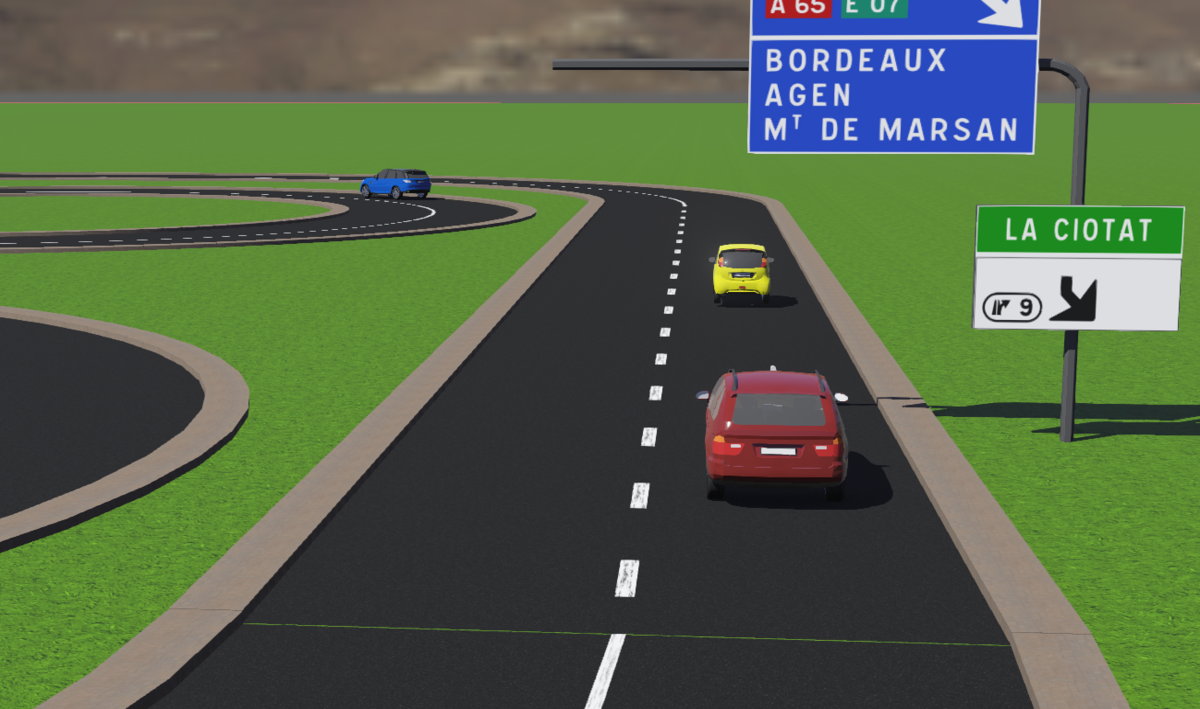
\includegraphics[width=0.5\textwidth]{Figures/Figures_Cap03/world_lanes.png}
    \caption{Carriles de la carretera.}
    \label{fig:world_lanes}
\end{figure}
Con la adición de otros vehículos dentro de la carretera se busca realizar detección y evasión de obstáculos, seguimiento y rebase de vehículos. El conjunto de estos objetos más otros elementos como: bordes en la carretera, áreas verdes e iluminación forman el escenario final donde se realizarán pruebas de conducción autónoma. Algunos elementos como: personas, mobiliario urbano, edificios, puentes, señales de tránsito y viales no se agregan al escenario ya que no resultan necesarias para este trabajo. El escenario final es el mostrado en \ref{fig:webots_world}.
\begin{figure}[h]
    \centering
    \begin{subfigure}[b]{0.4\textwidth}
         \centering
         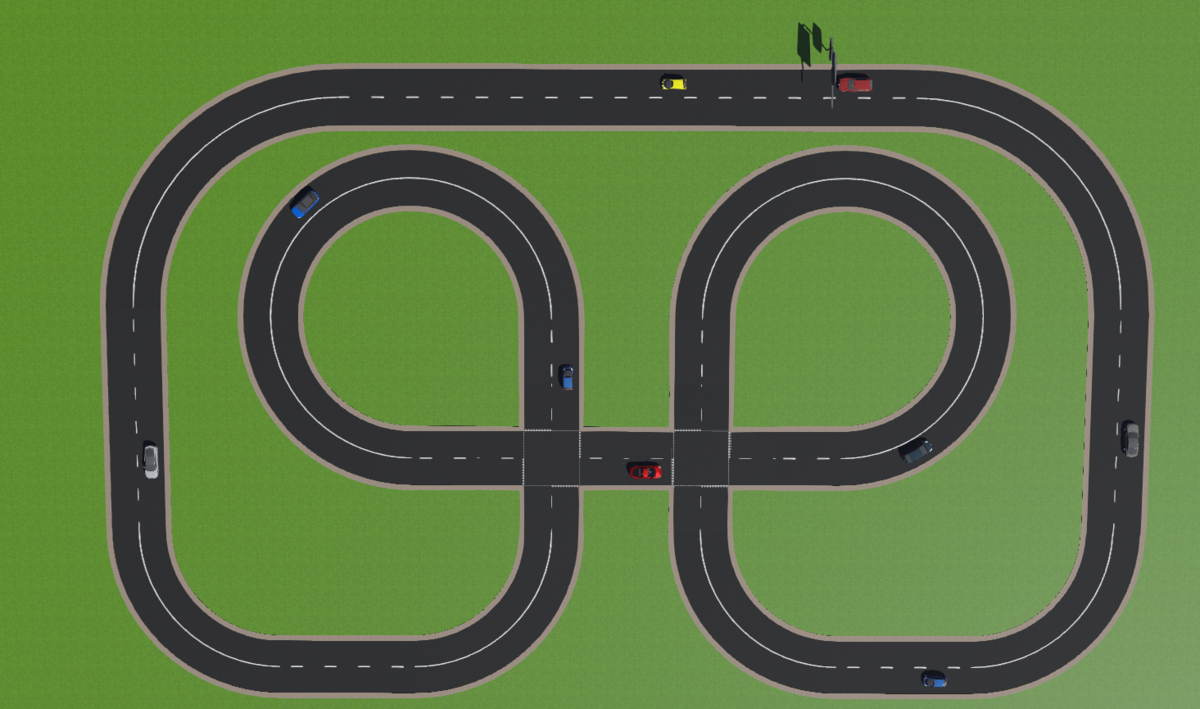
\includegraphics[width=\textwidth]{Figures/Figures_Cap03/webots_world.png}
         \caption{Escenario de pruebas de navegación.}
         \label{fig:webots_world}
    \end{subfigure}
    \hfill
    \begin{subfigure}[b]{0.375\textwidth}
         \centering
         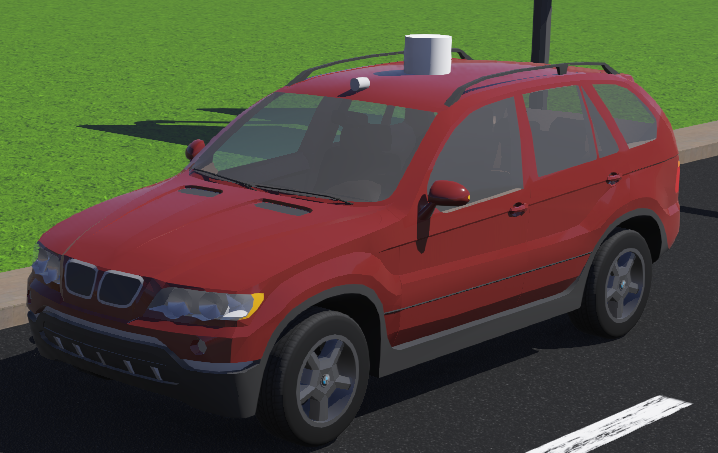
\includegraphics[width=\textwidth]{Figures/Figures_Cap03/test_car.png}
         \caption{Vehículo de pruebas instrumentado con sensores.}
         \label{fig:webots_car}
     \end{subfigure}
     
    \caption{Escenario y vehículo de pruebas.}
    \label{fig:world_car_test}
\end{figure}

En lo que respecta al vehículo de pruebas Webots incluye modelos de vehículos populares, estos modelos tienen características muy generales como, luces, llantas, tipo de motor, retrovisores, color y otros elementos comunes de un vehículo. Lo importante a destacar es que cada vehículo cuenta con secciones predefinidas para instrumentar el vehículo con los sensores necesarios. Para los propósitos de este proyecto se utiliza un vehículo 'X5' de 'BMW' en color rojo. A este vehículo se le añaden los siguientes sensores:
\begin{itemize}
    \item Cámara RGB, colocada en la parte frontal del vehículo.
    \item Lidar, colocado en la parte superior del vehículo.
    \item GPS, colocado en la parte frontal y superior del vehículo.
\end{itemize}

El vehículo para pruebas de navegación instrumentado con los sensores y actuadores necesarios se encuentra ilustrado en la figura \ref{fig:webots_car}.

Es es importante mencionar que el vehículo de pruebas 'BMW X5' es manipulado a través de un controlador, este se encarga de recibir información de cada sensor. Además, el mismo controlador envía señales para el control de velocidad, ángulo de dirección entre otros. En los próximos capítulos se ofrece una descripción con mayor detalle de cada uno de los nodos utilizados. En cuanto a los vehículos en movimiento dentro de la carretera se emplea un controlador supervisor para manipular la posición y velocidad de los vehículos.

\section{Contribuciones en el TMR} \label{sec:contribuciones_en_el_TMR}

El ambiente de simulación y vehículo de pruebas instrumentado fueron de ayuda en el desarrollo de la plataforma de uso para las pruebas consideradas en el TMR- AutoModelCar 2022 en su modalidad virtual. El uso de este simulador permitió generar los ambientes de simulación para las pruebas de:
\begin{itemize}
    \item Navegación autónoma sin obstáculos.
    \item Navegación autónoma con obstáculos estáticos.
    \item Navegación autónoma con obstáculos dinámicos.
    \item Estacionamiento autónomo.
\end{itemize}
Con ayuda del desarrollo de controladores supervisores se logró el control de posición y velocidad de los diferentes autos que actuaron como obstáculo en cada prueba. El desarrollo del controlador principal del vehículo de pruebas permitió el control de movimiento del mismo en base a los sensores integrados.
\\
\\

% CONCLUSIONES DEL CAPÍTULO
Al termino de este capítulo se entienden los conceptos básicos, ventajas y desventajas del simulador Webots. Además, se conoce el enfoque que se le dará al entorno de simulación en la búsqueda de implementar y probar algoritmos de navegación autónoma. Los escenarios modelados así como el vehículo de pruebas instrumentado en este capítulo son parte esencial en los capítulos siguientes, pues permitirán evaluar el desempeño de los algoritmos desarrollados y el comportamiento del vehículo en las diferentes situaciones que se le presenten.
\chapter{Seguimiento de carriles} \label{cap:seguimiento_de_carriles}
% BREVE DESCRIPCIÓN DEL CONTENIDO DE ESTE CAPÍTULO
Este capítulo se enfoca en hacer un primer reconocimiento del ambiente, se buscan identificar los carriles de la carretera, en especial, el carril donde se encuentra el vehículo autónomo. Al inicio, la sección \ref{sec:introducción_al_seguimiento_de_carriles} realiza una introducción para el proceso de seguimiento de carriles. A continuación, en \ref{sec:el_espacio_de_color_RGB} se define el concepto de espacio de color y algunas de las variantes más utilizadas, en la subsección \ref{sub:ejemplo_para_obtener_la_imagen_de_la_cámara} se muestra una forma de procesar una imagen RGB con la plataforma ROS. Enseguida, las secciones \ref{sec:detección_de_bordes} y \ref{sec:transformada_Hough} tratan de manera teórica los conceptos de detección de bordes de Canny y transformada Hough. Sus correspondientes subsecciones \ref{sub:ejemplo_para_detección_de_bordes_con_el_detector_de_canny} y \ref{sub:ejemplo_para_detección_de_líneas_rectas_con_transformada_Hough} son ejemplos de como implementar estas herramientas matemáticas en código de programación para aplicaciones de vehículos autónomos. Posteriormente, la sección \ref{sec:modelo_cinemático_del_vehículo} es una muestra del modelo cinemático del vehículo, siguiendo este modelo la sección \ref{sec:leyes_de_control} diseña las leyes de control correspondientes para el movimiento lateral y longitudinal del vehículo. Finalmente, se presentan los resultados de estas implementaciones.

Cabe mencionar que todas las implementaciones en código de algoritmos y pseudocódigos propuestos en este capítulo son desarrollados con el lenguaje de programación Python.

\section{Introducción al seguimiento de carriles} \label{sec:introducción_al_seguimiento_de_carriles}

El primer paso para cumplir con la tarea de navegación autónoma es el seguimiento de carriles, en un ambiente vial urbano los carriles son el principal indicador para mantener una ruta. Bajo este escenario, es fundamental contar con un instrumento que permita simular en medida de lo posible la visión humana, el sensor más cercano a este efecto es una cámara, con ella se puede conocer una parte del ambiente donde navegará el vehículo. Tal como se describió en la sección \ref{sec:el_ambiente_de_simulación} del capítulo \ref{cap:simulación_con_webots}, el vehículo autónomo modelado está instrumentado con una cámara digital en la parte superior para tener una imagen RGB frontal del ambiente. La imagen obtenida de la cámara es la principal fuente de información para supervisar el frente de la escena, está información (imagen) es procesada con el fin de identificar el carril donde debe conducir el vehículo autónomo y en base a ello calcular las leyes de control que permitan manipular las funciones operativas (movimiento lateral y longitudinal) del vehículo para mantenerse dentro del carril correspondiente en líneas curvas y rectas de la carretera. Para que el vehículo autónomo sea capaz de navegar bajo estas condiciones es recomendable separar el proceso en tareas más específicas, en concreto dos: Detección de carril y Seguimiento de Carril.

El reconocimiento del ambiente hace referencia a la detección del carril en el que debe mantenerse el vehículo, para realizar esta tarea se llevan a cabo los siguientes pasos:
\begin{enumerate}
    \item Obtener la información (imagen) de la cámara del vehículo.
    \item Determinar características de la imagen que ayuden en la detección del carril.
    \item Identificar las líneas que correspondan a los bordes del carril.
\end{enumerate}

La acción de seguimiento de carril se pretende conseguir mediante:
\begin{enumerate}
    \item Diseño e implementación de un control para velocidad y dirección del vehículo.
    \item Garantizar la seguridad del vehículo en todo momento.
\end{enumerate}

En las siguientes secciones de este capítulo se describen conceptos teórico matemáticos necesarios para el procesamiento digital de imágenes en la búsqueda de detección de carriles en la escena, además se ejemplifican los casos prácticos de cada una de las herramientas empleadas.

\section{El espacio de color RGB} \label{sec:el_espacio_de_color_RGB}

Dentro del procesamiento de imágenes es de suma importancia el uso de color por dos principales razones. En primer lugar, el color es un descriptor muy poderoso para la identificación y extracción de objetos de una escena. Por otra parte, los humanos podemos distinguir entre cientos de tonos de color pero solo un par de docenas en tonos de grises. Así, el procesamiento de imágenes a color se puede dividir en dos categorías: Procesamiento de Pseudo-color y Procesamiento de color completo. Para el procesamiento por Pseudo-color se emplea la asignación de color a una determinada intensidad de escala de grises mientras que en procesamiento de  color completo las imágenes se obtienen con ayuda de algún sensor a todo color(cámara digital, escáner a color) \cite{gonzalez2009digital}.

Un espacio de color es una forma para indicar como está definido un color, el propósito de un espacio de color, modelo de color o sistema de color como también es conocido consiste en facilitar la especificación de colores de una manera estándar. Es decir, es una especificación de un sistema de coordenadas y un sub-espacio dentro del sistema, de tal modo que cada color está representado por un solo punto contenido dentro del sub-espacio. En la práctica de procesamiento de imágenes los modelos de color más utilizados son el modelo RGB (Red, Green, Blue) para monitores de color, cámaras de vídeo; los modelos CMY (Cyan, Magenta, Yellow) y CMYK (Cyan, Magenta, Yellow, Black) son muy usados dentro de la industria de impresión de color. El modelos HSI (Hue, Saturation, Intensity) es el modelo que más se asemeja a la forma en que los humanos interpretamos el color, este modelo tiene la ventaja de poder desacoplar el color y el gris(escala de grises de una imagen) y por lo tanto es bastante común en el uso de técnicas de escala de grises\cite{gonzalez2009digital}.

El modelo de color RGB se basa en un sistema cartesiano de 3 coordenadas y el sub-espacio de interés es un cubo unitario. Es decir, se indica que todos los valores R, G y B se encuentran en un rango de [0, 1]. Dentro del espacio RGB, cada color aparece en su componente espectral primaria(R = 645.16nm, G = 526.32nm , B = 444.44nm)\cite{levinson2011towards}. El color negro se encuentra en el origen del cubo mientras que el blanco está situado en el vértice más lejano, los valores primarios (RGB) se sitúan en tres esquinas del cubo y los colores secundarios aparecen en las tres esquinas restantes. Los diferentes colores sobre o dentro del cubo están definidos por vectores que comienzan desde el origen. Además, la escala de grises (puntos donde los valores RGB son iguales) se extiende de negro a blanco a través de la línea que une estos dos vértices. La figura \ref{fig:rgb_cube} muestra la representación del espacio de color RGB.
\begin{figure}[h]
    \centering
    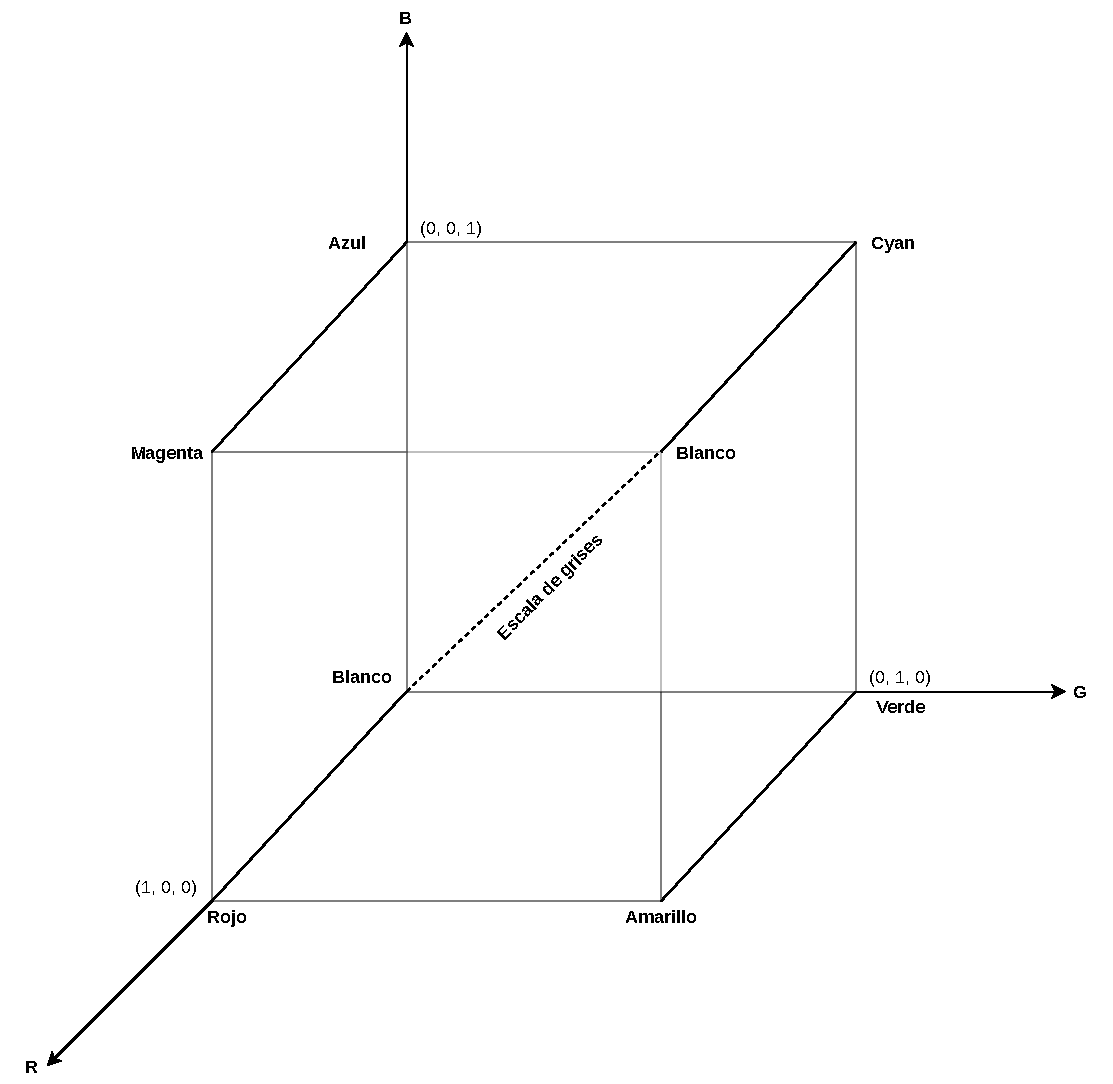
\includegraphics[width=0.75\textwidth]{Figures/Figures_Cap04/rgb_cube.pdf}
    \caption{Espacio RGB en coordenadas cartesianas.}
    \label{fig:rgb_cube}
\end{figure}

\subsection{Ejemplo para obtener la imagen de la cámara} \label{sub:ejemplo_para_obtener_la_imagen_de_la_cámara}

La cámara del vehículo provee una imagen en formato RGBA de 8-bits con dimensiones de ``640x480'' píxeles. A fin de obtener la imagen son necesarias las funciones especificas del nodo ``Camera'' del simulador Webots, además se hace uso de la plataforma ROS para el manejo de tópicos entre diferentes nodos, en específico se utiliza un mensaje del tipo \textit{Image} de ROS con la intención de publicar un tópico que contenga la información de la cámara. 

Para comenzar el procesamiento de la imagen se realiza una conversión de el mensaje \textit{Image} de ROS a una imagen tipo CV2 de OpenCV. Esto porque el mensaje \textit{Image} de ROS contiene la información de imagen en forma de lista donde el tamaño corresponde a el número de píxeles de la imagen (ancho por alto), en este caso el tamaño de la lista es de 640x480 = 307200. Cada uno de los elementos de la lista representa un píxel de la imagen en formato ARGB de 32 bits.

OpenCV es una biblioteca de código abierto para manipulación y procesamiento de imágenes, en adición con la alta compatibilidad entre la plataforma ROS y OpenCV son las principales razones para usar OpenCV dentro de este proyecto pues las funciones que ofrece son suficientes para cada uno de los pasos en el diseño de un algoritmo de detección carriles. Dentro de la plataforma ROS se encuentra un paquete llamado ``cv\_bridge'' el cual permite la conversión bilateral entre mensajes del tipo \textit{Image} de ROS e imágenes en formato OpenCV. La imagen \ref{fig:cv_bridge} ejemplifica la conversión entre estos dos tipos de mensajes.
% \footnote{\url{http://wiki.ros.org/cv_bridge/Tutorials}}
\begin{figure}
    \centering
    \begin{subfigure}[b]{0.4\textwidth}
         \centering
        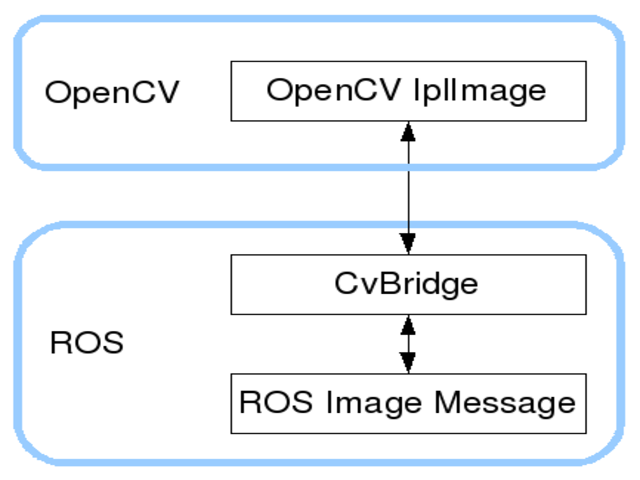
\includegraphics[width=\textwidth]{Figures/Figures_Cap04/cvbridge.png}
        \caption{Mensaje \textit{Image} de ROS a imagen de OpenCV.}
        \label{fig:cv_bridge}
    \end{subfigure}
    \hfill
    \begin{subfigure}[b]{0.4\textwidth}
        \centering
        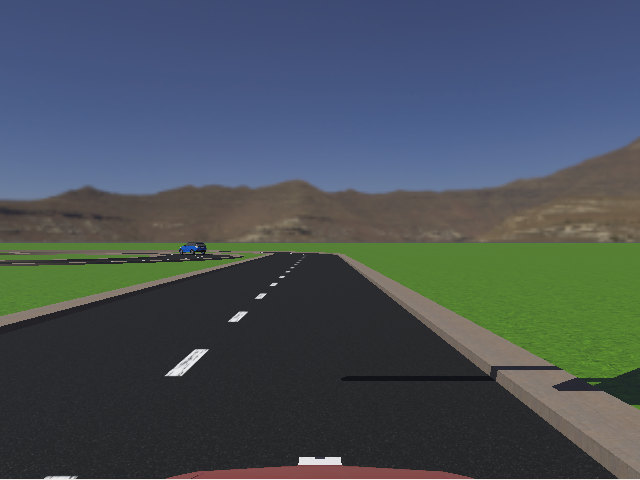
\includegraphics[width=\textwidth]{Figures/Figures_Cap04/lanes.png}
        \caption{Imagen de la cámara en formato de OpenCV.}
        \label{fig:lanes_cv}
    \end{subfigure}
    \caption{Resultado de transformar un mensaje \textit{Image} de ROS a una imagen de OpenCV.}
    \textit{Nota}. (a) Tomada de \textit{Stechschulte}, 2020 \cite{cv_bridge}.
    \label{fig:ros_cv}
\end{figure}

Referente a la implementación de código, la principal fuente información es proporcionada en la documentación oficial de OpenCV, disponible en \footnote{\url{https://opencv.org/}}. A continuación se muestra el código necesario para el tratado de un mensaje \textit{Image} de ROS y la conversión a imagen de OpenCV. En \ref{fig:lanes_cv} se ilustra el resultado de la imagen obtenida.

\begin{lstlisting}[language=Python]
from cv_bridge import CvBridge

bridge = CvBridge()
cv2_img = bridge.imgmsg_to_cv2(msg, 'bgr8')
\end{lstlisting}

\section{Detección de bordes} \label{sec:detección_de_bordes}

La detección de bordes es una herramienta en el procesamiento de imágenes diseñada para detectar píxeles de borde. Los píxeles de borde son píxeles donde la intensidad de una imagen cambia abruptamente y los bordes son conjuntos de píxeles entre bordes conectados. Es decir, la detección de bordes se utiliza para segmentar imágenes en función de cambios bruscos de intensidad. 

Dentro de este contexto existen diferentes formas de modelar un borde, una muy utilizada clasificación es usar como criterio la intensidad. Este escenario contempla: \textit{Step Edge} o borde de paso, como aquél que se presenta cuando existe una transición entre dos niveles de intensidad en distancia de un píxel. En la práctica es muy común encontrar imágenes distorsionadas por ruido o por algún filtro añadido previamente, de manera coloquial se entiende que la imagen se ve borrosa. En tales situaciones se pueden modelar bordes mediante una rampa de intensidad \textit{Ramp Edge}, donde la pendiente de la rampa es inversamente proporcional al grado de desenfoque, ya que no se cuenta con un solo punto de borde, cada punto dentro de la rampa es un punto borde aceptable, de esta manera un segmento de borde es un conjunto de puntos situados en la rampa. Como tercer tipo de borde está \textit{Roof Edge} o borde de techo, los bordes de techo son modelos de líneas dentro de una región, donde el ancho del borde es determinado por medio del grosor y nitidez de la línea, es normal encontrar bordes de techo en digitalización de dibujos e imágenes satélites\cite{gonzalez2009digital}. La figura \ref{fig:edges_types} ejemplifica los tres tipos de bordes descritos.
% \footnote{\url{https://www.ics.uci.edu}}
\begin{figure}[h]
    \centering
    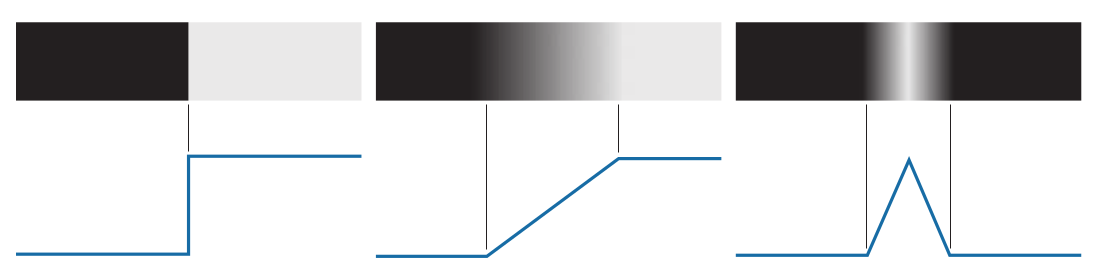
\includegraphics[width=0.75\textwidth]{Figures/Figures_Cap04/edge_type.png}
    \caption{Tipos de Bordes.}
    \textit{Nota}. Tomada de \textit{Gonzalez}, 2009 \cite{gonzalez2009digital}.
    \label{fig:edges_types}
\end{figure}

Los bordes mencionados anteriormente son los más comunes y utilizados por algoritmos de detección de bordes, debido a que son comportamientos muy frecuentes en imágenes. En general, un algoritmo de detección de bordes consta de tres pasos esenciales:
\begin{enumerate}
    \item Suavizar la imagen para reducir ruido.
    \item Detectar puntos borde (Puntos potenciales para ser candidatos a puntos de borde).
    \item Localizar bordes (Selección de puntos candidatos que pertenecen a un borde).
\end{enumerate}

\subsection{Detector de bordes de Canny} \label{sub:detector_de_bordes_de_canny}

Desarrollado en 1986 por John F. Canny, es un algoritmo para detección de bordes con mayor complejidad que los algoritmos tradicionales. Sin embargo, el rendimiento de este también resulta ser superior. El enfoque de este algoritmo se basa en tres principales objetivos:
\begin{enumerate}
    \item Tasa de error baja. Se deben localizar todos los bordes y no deben existir respuestas ilegítimas.
    \item Los puntos borde deben ser bien ubicados. Los bordes detectados deben estar lo más cercano posible a los bordes verdaderos. Es decir, debe existir distancia mínima entre ellos.
    \item Respuesta única de punto de borde. El detector debe devolver solo un punto borde por cada punto de borde verdadero. 
\end{enumerate}

El funcionamiento para detección de bordes mediante el algoritmo de Canny se fundamenta en el uso del vector gradiente debido a que este vector cuenta con la conocida propiedad de apuntar en la dirección de máxima tasa de cambio \cite{gonzalez2009digital}. El vector gradiente de una imagen se define en la ecuación (\ref{eqn:img_gradient}):
\begin{equation}
    \nabla f(x, y) \equiv grad[f(x, y)] \equiv \begin{bmatrix} 
        g_x(x, y) \\
        \\
        g_y(x, y) 
    \end{bmatrix}
    = 
    \begin{bmatrix} 
        \frac{\partial f(x, y)}{\partial x}\\
        \\
        \frac{\partial f(x, y)}{\partial y}
    \end{bmatrix}
    \label{eqn:img_gradient}
\end{equation}

Esta herramienta permite determinar la magnitud y dirección de un borde, donde la magnitud $M(x, y)$  es el valor de la tasa de cambio en la dirección del gradiente y está compuesta por su norma vectorial euclidiana.
\begin{equation}
    M(x, y) = \nabla \|f(x, y)\| = \sqrt{g_x^2(x, y) + g_y^2(x, y)}
\end{equation}

La dirección del vector gradiente en un punto $(x, y)$ está dada por:
\begin{equation}
    \alpha (x, y) = \tan^{-1} \begin{bmatrix}
        \frac{g_y(x, y)}{g_x(x, y)}
    \end{bmatrix}
\end{equation}

El algoritmo para detección de bordes de Canny consta de los siguientes pasos.
\begin{enumerate}
    \item Aplicar filtro gaussiano a la imagen de entrada para disminuir ruido.
    \item Calcular magnitud y ángulo del vector gradiente.
    \item Suprimir puntos no máximos.
    \item Detectar y vincular bordes mediante aplicación de doble umbralización.
\end{enumerate}

\subsection{Ejemplo para detección de bordes con el detector de Canny} \label{sub:ejemplo_para_detección_de_bordes_con_el_detector_de_canny}

%Se puede afirmar que los bordes son una poderosa característica para obtener información concreta de una escena. En la detección de carriles como primer paso se pretenden calcular los bordes contenidos en toda la imagen con el fin de contar con elementos suficientes que describan cada uno de los objetos presentes. 
El algoritmo de bordes de Canny es la herramienta seleccionada para lograr el proceso de extraer los bordes que representan los carriles de la carretera, en específico las líneas que conforman los bordes del carril donde se encuentra el auto de pruebas. OpenCV provee una función para utilizar el algoritmo de Canny, en breve se presenta la sección de código donde se hace uso de la función ``Canny()'' de OpenCV.

\begin{lstlisting}[language=Python]
import cv2

def canny(image):

    gray = cv2.cvtColor(image, cv2.COLOR_RGB2GRAY)  
    blur = cv2.GaussianBlur(gray, (5, 5), 0)        
    canny = cv2.Canny(blur, 50, 150)                
    return canny
\end{lstlisting}

El código anterior expone la forma de usar la función ``Canny()'' de OpenCV para detección de bordes. En la primer sentencia (línea 5) se realiza una conversión entre espacios de color, en específico de una imagen RGB a una imagen en escala de grises, el segundo paso (línea 6) tiene aplica un filtro Gaussiano a la imagen en escala de grises para reducir ruido. Finalmente en la línea 7 se aplica en concreto la función 'cv2.Canny()' para obtener una imagen en blanco y negro que contiene los bordes detectados por ``Canny()''.

La imagen \ref{fig:lanes_comparsion}, ofrece una comparación entre la imagen original \ref{fig:lanes} obtenida de la cámara y la imagen de bordes alcanzada por el algoritmo de Canny \ref{fig:edges_lanes}. El resultado de está operación es muy importante para el siguiente paso en la detección los carriles.
\begin{figure}[h]
    \centering
    \begin{subfigure}[b]{0.4\textwidth}
         \centering
         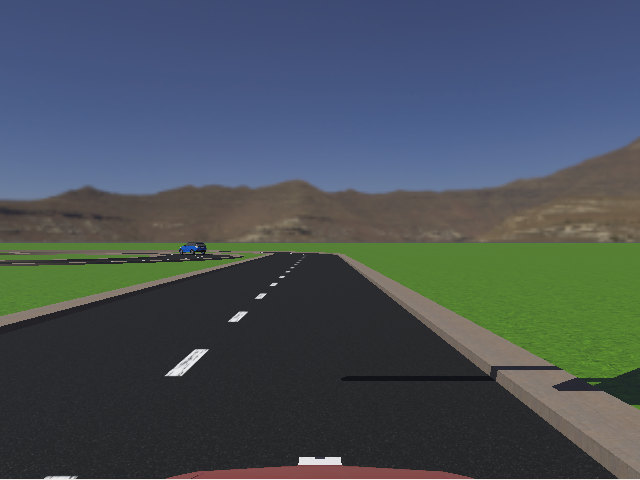
\includegraphics[width=\textwidth]{Figures/Figures_Cap04/lanes.png}
         \caption{Imagen original.}
         \label{fig:lanes}
    \end{subfigure}
    \hfill
    \begin{subfigure}[b]{0.4\textwidth}
         \centering
         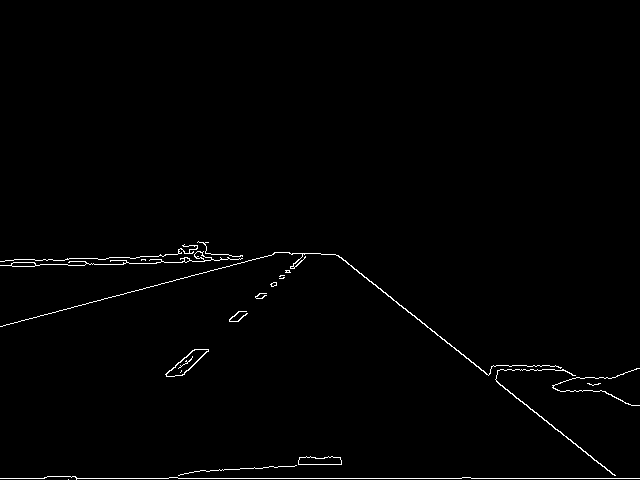
\includegraphics[width=\textwidth]{Figures/Figures_Cap04/edge_lanes.png}
         \caption{Imagen de Bordes.}
         \label{fig:edges_lanes}
     \end{subfigure}
     
    \caption{Comparación en entre la imagen original y la imagen de bordes.}
    \label{fig:lanes_comparsion}
\end{figure}

\section{Transformada Hough} \label{sec:transformada_Hough}

Buscar formas dentro de una imagen digital es una tarea común en el procesamiento de imágenes, en muchas de las ocasiones se buscan ajustar un conjunto de puntos en una determinada estructura, ya sean líneas rectas, círculos o alguna otra geometría. La transformada de Hough es una técnica propuesta por Paul Hough en 1962 y ampliamente utilizada dentro del campo de visión computacional para detección de líneas rectas y curvas en imágenes a color y en escala de grises.

El algoritmo busca identificar formas básicas en una imagen haciendo uso de los parámetros que describen la geometría deseada. Dentro de este concepto la transformada de Hough funciona a través de un sistema de votación, es decir, se identifica una forma específica si se obtiene un número suficiente de votos. Mediante esta técnica es posible encontrar cualquier figura que pueda ser expresada matemáticamente, el caso más sencillo es la detección de líneas rectas \cite{forsyth2011computer}.

\subsection{Detección de líneas rectas mediante transformada Hough} \label{sub:detección_de_líneas_rectas_mediante_transformada_Hough}

Dentro del espacio de imagen una línea puede ser expresada en un sistema cartesiano mediante los parámetros $(m, b)$ con la ecuación:
\begin{equation}
    y = mx + b
\end{equation}
mientras que en un sistema polar con los parámetros $(\rho, \theta)$ como:
\begin{equation}
    \rho = x \cos{\theta} + y \sin{\theta}
    \label{eqn:polar_line} 
\end{equation}

El principio fundamental del algoritmo de Hough para detección de líneas rectas consiste en trazar $n$ cantidad de líneas rectas para cada punto de la imagen y mediante el sistema de votación determinar que puntos forman una línea. Para la transformada de Hough resulta más sencillo trabajar en un sistema polar con los parámetros $(\rho, \theta)$, debido a que para cualquier punto de la imagen existen una infinidad de líneas que pasan a través de él, en el caso de líneas verticales los parámetros $(m, b)$ están indefinidos, en un sistema polar no existe este problema pues para líneas verticales se tiene $\theta = 90^\circ$ y para líneas horizontales $\theta = 0^\circ$. De esta manera se evita cualquier tipo de discontinuidad. Además, en la forma polar si la línea corresponde a un borde, el ángulo $\theta$ es la dirección del gradiente \cite{gonzalez2009digital}.

Como se mencionó anteriormente en cada punto de la imagen se trazan $n$ líneas, teniendo en cuenta esto es evidente que al menos una de las $n$ líneas atraviesa dos o más puntos de la imagen, es decir, los puntos sobre la recta tienen la propiedad de ser colineales, este es el sistema de votación que utiliza el algoritmo de Hough, pues entre más puntos estén contenidos dentro de una recta más votos tendrá, como consecuencia la recta con el mayor número de votos será considerada como una línea recta identificada dentro de la imagen.

Tomado como ejemplo la imagen \ref{fig:cartesian_space} se tienen dos puntos $(x_i, y_i)$ y $(x_j, y_j)$ en el espacio de imagen contenidos en el plano $xy$, la recta azul $L$ representa una recta en forma polar con parámetros $(\rho, \theta)$ que pasa a través de los puntos $(x_i, y_i)$ y $(x_j, y_j)$. Esta línea $L$ en el espacio cartesiano corresponde a un punto $P_h$ en el espacio de Hough con coordenadas $(\rho', \theta')$ en \ref{fig:hough_space}. Un punto $P(x_i, y_i)$ en el espacio cartesiano corresponde a una curva $C_i$ en el espacio de Hough, donde $C_i$ es  representada por los parámetros $(\rho_i, \theta_i)$ de todas las rectas $L_i$ que pasan por el punto $P(x_i, y_i)$ en el espacio cartesiano calculados mediante la ecuación (\ref{eqn:polar_line}), la imagen \ref{fig:hough_space} muestra la familia de curvas $C$ que pasan a través del punto $P_h$ en el espacio de Hough.

Finalmente el método de votación del algoritmo de Hough consiste en encontrar las curvas $C_i$ dentro del espacio de Hough que pasan a través del punto $P(x_i, y_i)$ del espacio cartesiano. Los puntos $P_h$, es decir la intersección $(\rho ', \theta')$ en el espacio de Hough por donde pasen más curvas $C_i$ serán las rectas resultantes en el espacio cartesiano.
\begin{figure}
    \centering
    \begin{subfigure}[b]{0.4\textwidth}
         \centering
         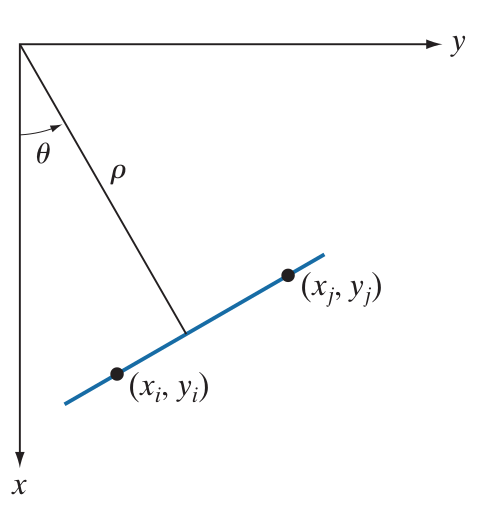
\includegraphics[width=\textwidth]{Figures/Figures_Cap04/cartesian_space.png}
         \caption{Parametrización de una recta en el plano $xy$.}
         \label{fig:cartesian_space}
    \end{subfigure}
    \hfill
    \begin{subfigure}[b]{0.42\textwidth}
         \centering
         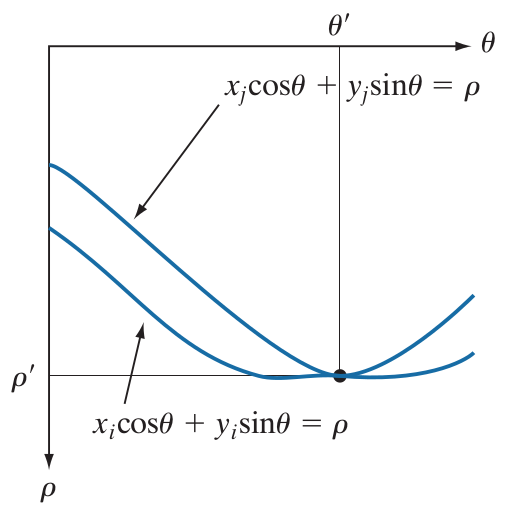
\includegraphics[width=\textwidth]{Figures/Figures_Cap04/hough_space.png}
         \caption{Familia de Curvas en el espacio de Hough.}
         \label{fig:hough_space}
     \end{subfigure}
     
    \caption{Interpretación geométrica de los espacios cartesiano y de Hough.}
    \textit{Nota}. Tomadas de \textit{Gonzalez}, 2009 \cite{gonzalez2009digital}.
    \label{fig:cartesian_hough_space}
\end{figure}

\subsection{Ejemplo para detección de líneas rectas con transformada Hough} \label{sub:ejemplo_para_detección_de_líneas_rectas_con_transformada_Hough}

Para continuar con el proceso de detección de carril es necesario identificar las líneas que los conforman, ver \ref{fig:lanes}. La manera más sencilla de encontrar un carril dentro de una imagen es delimitar el espacio donde se encuentra. Un carril está contenido por dos líneas rectas paralelas que pueden ser continuas, discontinuas e incluso líneas rectas dobles. El problema que se presenta en este caso es la detección de líneas rectas y el enfoque de la transformada de Hough para líneas rectas es justo la herramienta que permite resolver este problema. 

Los párrafos siguientes describen una forma en que se puede usar la transformada de Hough para detección de líneas rectas e identificar las líneas que forman un carril.

Es importante mencionar que la transformada de Hough para detección de líneas rectas produce un mejor resultado con una imagen que presente solo la información de los bordes y en una escala de grises o bien en blanco y negro, este requisito justifica el hecho de haber detectado los bordes de la imagen de la cámara del vehículo de pruebas con el algoritmo de Canny, pues con está imagen se obtendrán las líneas que forman el carril donde se encuentra el vehículo. Sin embargo, no todos los bordes de la imagen son necesarios, por ello es necesario delimitar solo el área de interés donde se encuentra el carril, una vez determinada el área de interés es más fácil y eficiente obtener las líneas pertenecientes al carril.

El proceso de detección de carril mediante líneas rectas requiere definir el área donde está situado el carril de interés, este procedimiento se describe a continuación:
\begin{enumerate}
    \item Obtener una imagen con los bordes de la imagen original, ver \ref{fig:edge_lines}.
    
    \item Delimitar el perímetro donde se encuentra el carril a través de una geometría que pueda ser descrita mediante líneas rectas. Un triángulo es la geometría que mejor se adecua en este caso particular ver, \ref{fig:triangle_interest}.
    
    \item Descartar los bordes que se encuentren fuera de la región de interés para solo contar con los bordes que corresponden a la geometría del carril, ver \ref{fig:lanes_interest}.
\end{enumerate}

\begin{figure}[h]
    \centering
    \begin{subfigure}[b]{0.3\textwidth}
         \centering
         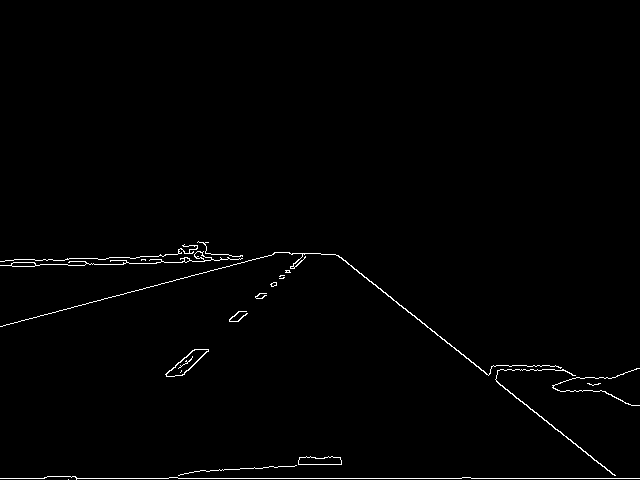
\includegraphics[width=\textwidth]{Figures/Figures_Cap04/edge_lanes.png}
         \caption{Imagen de bordes.}
         \label{fig:edge_lines}
    \end{subfigure}
    \hfill
    \begin{subfigure}[b]{0.3\textwidth}
         \centering
         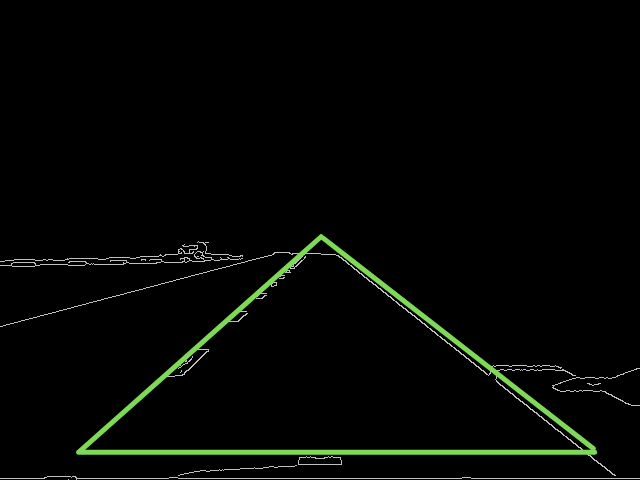
\includegraphics[width=\textwidth]{Figures/Figures_Cap04/triangle_of_interest.png}
         \caption{Triángulo de interés.}
         \label{fig:triangle_interest}
     \end{subfigure}
     \hfill
     \begin{subfigure}[b]{0.3\textwidth}
         \centering
         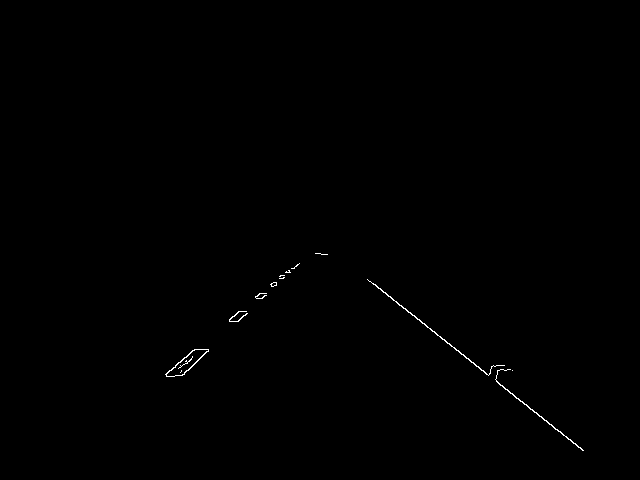
\includegraphics[width=\textwidth]{Figures/Figures_Cap04/lanes_cropped.png}
         \caption{Bordes de interés.}
         \label{fig:lanes_interest}
     \end{subfigure}
     
    \caption{Proceso para delimitar la región de interés de el carril.}
    \label{fig:interest_region}
\end{figure}

\newpage
Previamente se realizó la detección de bordes en la imagen. Ahora es turno de delimitar la zona del carril, la implementación en código para definir el área de interés es la siguiente:

\hfill
\begin{lstlisting}[language=Python]
import cv2
import numpy as np

def region_of_interest(image):
    triangle = np.array( [ (0, 450), (640, 450), (320, 250) ])
    mask = np.zeros_like(image)
    cv2.fillPoly(mask, triangle, 255)
    cropped_img = cv2.bitwise_and(image, mask)
    
    return cropped_img

canny_img = canny(lane_img)                                                 
cropped_img = region_of_interest(canny_img)         
\end{lstlisting}
\hfill

Donde la línea 12 contiene la imagen de bordes obtenidos de la imagen original. A partir de la línea 4 se define la función ``region\_of\_interest()'' para calcular la región de interés, esta función recibe como parámetro la imagen de bordes. En la línea 5 se forma el perímetro del triángulo que contiene los bordes necesarios para identificar el carril, por último la línea 8 secciona la imagen de bordes y solo permanecen los bordes que forman el carril de interés. En \ref{fig:lanes_interest} se ilustra el resultado de la ejecución de este desarrollo.

La tarea más importante en la detección de las líneas que forman el carril es el uso de la transformada Hough para líneas rectas, en breve se enuncian los pasos para obtener las líneas resultantes de el carril.

\begin{enumerate}
    \item Aplicar transformada de Hough a la imagen que contiene los bordes de la región de interés.
    \item Identificar las líneas resultantes con el propósito de saber a que borde del carril pertenecen (izquierdo o derecho).
    \begin{itemize}
        \item Para obtener el conjunto de líneas pertenecientes a cada borde se utiliza la pendiente de las rectas detectadas con Hough como diferenciador. En el caso rectas pertenecientes al borde izquierdo del carril $m > 0$, es decir, pendiente positiva y para el borde derecho se tienen rectas con $m < 0$, pendiente negativa. Líneas horizontales son despreciadas.
    \end{itemize}
    \item Obtener un promedio para cada conjunto de líneas debido a que el carril de una carretera cuenta con solo dos líneas rectas (izquierda y derecha), por esta razón es necesario obtener una sola línea del conjunto de rectas pertenecientes a cada grupo que se ajuste bien en cada borde del carril.
    \item Ilustrar el resultado final de las dos líneas rectas con coordenadas cartesianas para comprobar que la detección de carril es correcta.
\end{enumerate}

La línea 1 en la siguiente porción de código es la forma de usar la función que provee OpenCV para la transformada de Hough, donde su primer parámetro es la imagen de bordes pertenecientes a la región del carril que se obtuvo previamente, los parámetros restantes son constantes que requiere la función, estos valores son recomendados en la documentación de OpenCV. Como efecto de esta operación se extraen las líneas rectas detectadas, estas líneas se ilustran en la figura \ref{fig:hough_lines}.

\hfill
\begin{lstlisting}[language=Python]
lines = cv2.HoughLinesP(
            cropped_img,
            2,
            np.pi/180,
            80,
            minLineLength=40,
            maxLineGap=50
        )
\end{lstlisting}
\hfill

Como lo indican los pasos descritos en está sección se deben de filtrar las líneas detectadas en dos grupos (izquierdas y derechas) para poder calcular un promedio por grupo y generar una sola línea en cada borde del carril. La función que realiza este proceso es la siguiente:

\hfill
\begin{lstlisting}[language=Python]
def avg_slope_intercept(image, lines):
    if angle < -0.3 or angle > 0.3:
        if slope < 0:
            right_fit.append((slope, intercept))    
        else:
            left_fit.append((slope, intercept)) 
    
    left_line_avg = np.average(left_fit, axis=0)    
    right_line_avg = np.average(right_fit, axis=0) 
\end{lstlisting}
\hfill

Donde la distribución de líneas detectadas en cada grupo se inicia en la línea 2, en primer lugar se desprecian aquellas líneas con ángulo de inclinación $\theta$ en rango de [-0.3, 0.3] radianes porque estás líneas representan aquellas que son horizontales o están muy cerca de ser horizontales y pueden provocar imprecisiones en el resultado final. A partir de la línea 3 se inicia la condición para dividir en grupos de rectas izquierdas o derechas con la pendiente como diferenciador, $m < 0$ para líneas rectas del borde derecho y $m > 0$ para líneas rectas del borde izquierdo. Finalmente las líneas 8 y 9 contienen el resultado de calcular el promedio de las líneas del borde derecho e izquierdo respectivamente y como consecuencia tener una sola línea por borde tal como se muestra en \ref{fig:avg_lines}. Para ejemplificar el resultado final de la detección de carriles se genera la imagen \ref{fig:combo_img}, donde se muestra la imagen original, las líneas del carril detectadas son colocadas en color azul, esta imagen permite demostrar que la detección del carril funciona correctamente, pues las líneas rectas detectadas se encuentran sobrepuestas en el carril real.
\begin{figure}[h]
    \centering
    \begin{subfigure}[b]{0.3\textwidth}
         \centering
         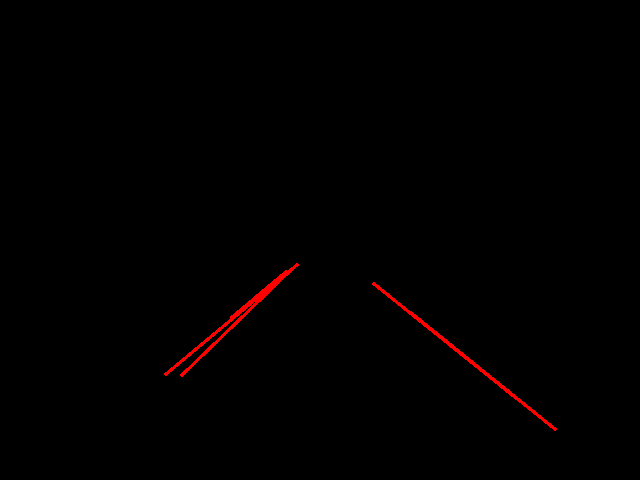
\includegraphics[width=\textwidth]{Figures/Figures_Cap04/hough_lines.png}
         \caption{Líneas detectadas.}
         \label{fig:hough_lines}
    \end{subfigure}
    \hfill
    \begin{subfigure}[b]{0.3\textwidth}
         \centering
         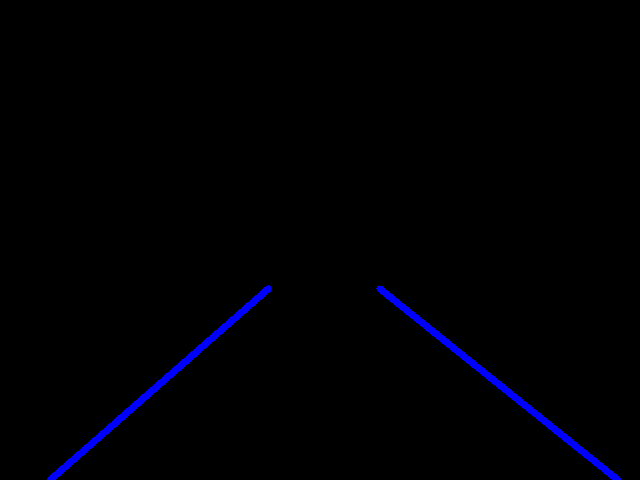
\includegraphics[width=\textwidth]{Figures/Figures_Cap04/avg_hough_lines.png}
         \caption{Líneas promedio.}
         \label{fig:avg_lines}
     \end{subfigure}
     \hfill
     \begin{subfigure}[b]{0.3\textwidth}
         \centering
         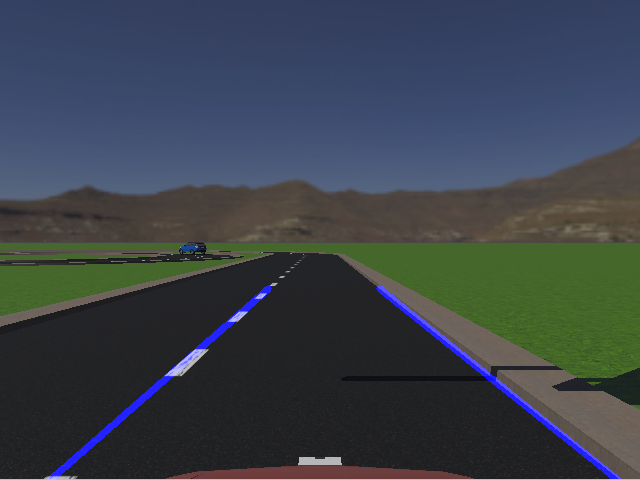
\includegraphics[width=\textwidth]{Figures/Figures_Cap04/combo_img.png}
         \caption{Carril detectado.}
         \label{fig:combo_img}
     \end{subfigure}
     
    \caption{Líneas del carril detectadas por medio de Transformada Hough.}
    \label{fig:lane_detect}
\end{figure}

El resultado del proceso de detección de carril finaliza con la obtención de las líneas que conforman los bordes del carril en coordenadas cartesianas. Estas líneas servirán como modelo en el cálculo de las leyes de control para la tarea de seguimiento de carril donde se involucra velocidad y ángulo de dirección.

\section{Modelo cinemático del vehículo} \label{sec:modelo_cinemático_del_vehículo}

El modelo cinemático es una descripción del movimiento realizado por el Robot en función de su geometría. La cinemática del Robot puede utilizarse como modelo matemático de partida en el diseño de un controlador, para simular el comportamiento cinemático, o para establecer ecuaciones en cálculos de odometría \cite{martinez2003modelado}. 

Para el caso del modelo cinemático del vehículo autónomo se considera el llamado modelo de vía única o \textit{Single-Track-Model} en inglés. En el modelo de única vía, el vehículo cuenta con dos ruedas que están unidas a través de un eslabón que está comprometido a moverse en un plano. Se parte del supuesto que las ruedas pueden girar libremente sobre sus ejes de rotación y que las ruedas no patinan sobre el punto de contacto con el suelo. Además, para modelar la dirección (\textit{steering}) la rueda delantera cuenta con un grado adicional de libertad que le permite girar sobre un eje normal al plano de movimiento. Con estas dos características se refleja la experiencia que tienen los conductores cuando el vehículo no realiza movimiento lateral sin previamente haber avanzado \cite{paden2016survey}. 

Considerando la figura \ref{fig:single_track_model}, donde $p_r$ y $p_f$ son los puntos de contacto con el suelo para los neumáticos trasero y delantero respectivamente, $\theta$ es el ángulo que describe la dirección hacia donde mira el vehículo y $\delta$ es el ángulo de dirección para la rueda delantera. Todo esto en un sistema de coordenadas inercial con vectores base $(\hat{e}_{x}, \hat{e}_{y})$.
% La limitación de maniobras en este modelo se denomina restricción no holonómica y es una restricción diferencial sobre el movimiento del vehículo.
Para satisfacer el supuesto de no deslizamiento, el movimiento de los puntos $p_r$ y $p_f$ debe de ser colineal respecto a la orientación de la rueda. Esta restricción para la llanta trasera se expresa como:
\begin{equation}
    (\dot{p}_r \cdot \hat{e}_y)\cos{(\theta)} - (\dot{p}_r \cdot \hat{e}_x)\sin{(\theta)} = 0
\end{equation}
y para la llanta delantera:
\begin{equation}
    (\dot{p}_f \cdot \hat{e}_y)\cos{(\theta + \delta)} - (\dot{p}_f \cdot \hat{e}_x)\sin{(\theta + \delta)} = 0
\end{equation}

\begin{figure}[h]
    \centering
    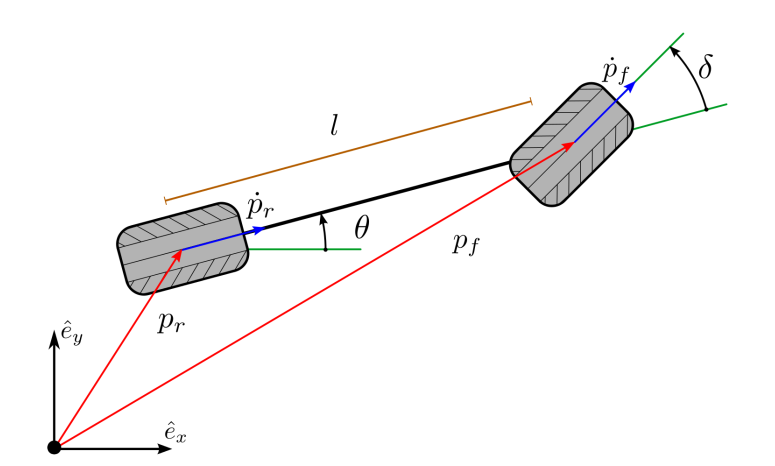
\includegraphics[width=0.5\textwidth]{Figures/Figures_Cap04/single_track_model.png}
    \caption{Modelo cinemático de vía única (\textit{Single-Track Model}).}
    \textit{Nota}. Tomada de \textit{Paden}, 2016 \cite{paden2016survey}.
    \label{fig:single_track_model}
\end{figure}


Por lo general estas expresiones se reordenan en términos del movimiento en cada punto de los vectores base $(\hat{e}_{x}, \hat{e}_{y})$. El movimiento de la llanta trasera a lo largo de $\hat{e}_{x}$ es $x_r := p_r \cdot \hat{e}_x$. Para la dirección $\hat{e}_{y}$, $y_r := p_r \cdot \hat{e}_y$. La velocidad de movimiento es la magnitud de $\dot{p}_r$ con el signo correcto para indicar conducción hacia adelante o en reversa. 

En términos de cantidades escalares $x_r$, $y_r$ y $\theta$, la restricción diferencial es:
\begin{equation}
    \begin{split}
        \dot{x}_r & = v_r \cos{(\theta)} \\
        \dot{y}_r & = v_r \sin{(\theta)} \\
        \dot{\theta}_r & = \frac{v_r}{l}\tan{(\theta)}
    \end{split}
\end{equation}

Alternativamente se puede escribir la misma restricción diferencial en términos del movimiento de la rueda delantera.
\begin{equation}
    \begin{split}
        \dot{x}_f & = v_f \cos{(\theta + \delta)} \\
        \dot{y}_f & = v_f \sin{(\theta + \delta)} \\
        \dot{\theta}_f & = \frac{v_f}{l}\sin{(\delta)}
        \label{eqn:front_whell}
    \end{split}
\end{equation}

pero ahora se utiliza la velocidad de la rueda delantera, esta velocidad está relacionada con la velocidad de la llanta trasera por:
\begin{equation}
    \frac{v_r}{v_f} = \cos{(\delta)}
\end{equation}

Los problemas de control de este modelo pueden implicar el seleccionar un ángulo de dirección $\delta$ dentro de los rangos mecánicos aceptables por el vehículo, $ \delta \in [\delta_{min}, \delta_{max}]$ , y mantener la velocidad de avance en un rango estable, $v_r \in [v_{min}, v_{max}]$. Otro inconveniente importante de este modelo es que permite cambios instantáneos en el ángulo de dirección y por ende provocar cambios bruscos en la dirección.

La continuidad del ángulo de dirección para la rueda delantera se pude imponer añadiendo una velocidad más en la ecuación (\ref{eqn:front_whell}), donde el ángulo de dirección integra una velocidad constante. Entonces, la ecuación (\ref{eqn:front_whell}) se reescribe como:
\begin{equation}
    \begin{split}
        \dot{x}_f & = v_f \cos{(\theta + \delta)} \\
        \dot{y}_f & = v_f \sin{(\theta + \delta)} \\
        \dot{\theta}_f & = \frac{v_f}{l}\sin{(\delta)} \\
        \dot{\delta} & = v_{\delta}
    \end{split}
\end{equation}
Ahora, además de limitar el ángulo de dirección también se puede limitar la velocidad en la dirección para la rueda del frente, $v_{\delta} \in [\dot{\delta}_{min}, \dot{\delta}_{max}]$. Este mismo problema se puede presentar con la velocidad del automóvil descrita por $v_r$ y se puede abordar de la misma manera. El único inconveniente de esta técnica es que el aumento en la dimensión del modelo podría complicar más los problemas de planificación y control del movimiento.

Más adelante se considerará este modelo cinemático para el diseño de las leyes de control que influyan en el movimiento lateral y longitudinal del vehículo autónomo. En concreto, la relación que existe con el movimiento de la rueda delantera y el rango del ángulo de dirección (\textit{steering}).

\section{Leyes de control} \label{sec:leyes_de_control}

Un controlador es un componente que permite procesar información de sensores y generar salidas específicas. La forma en que un controlador opera sobre una señal se conoce como algoritmo de control o ley de control.
% La forma en que un controlador opera sobre una señal de error
El objetivo de una ley de control es ajustar el valor de una señal respecto a un valor conocido, el cual puede provenir de la lectura de un sensor o bien ser el resultado de una operación previa. La diferencia entre valor conocido y valor medido se conoce como error. Una ley de control actúa sobre el error a través de algún mecanismo y manipula el proceso para provocar la salida esperada. Es decir, se pretende que la ley de control pueda compensar efectos de los elementos dinámicos del sistema \cite{gonzalez2015review}.

En este proyecto se busca calcular un error con base en las líneas observadas de los bordes del carril en la sección \ref{sub:ejemplo_para_detección_de_líneas_rectas_con_transformada_Hough} y las líneas reales de los bordes del carril, este error permitirá diseñar un ley de control para el movimiento lateral del vehículo con base en el modelo cinemático. Mediante esta ley de control el vehículo debe ser capaz de controlar el ángulo de dirección (\textit{steering})
en un rango estable para mantenerse dentro del carril en líneas rectas, curvas a la derecha y curvas hacia la izquierda.


\subsection{Diseño e implementación de una ley de control para movimiento lateral del vehículo} \label{sub:diseño_e_implementación_de_una_ley_de_control_para_movimiento_lateral_del_vehículo}

En la búsqueda de mantener el vehículo autónomo alineado y dentro de su carril se deben diseñar leyes de control que faciliten el proceso de seguimiento de carril, el objetivo de las leyes de control es manipular el error entre líneas observadas y líneas reales del carril para posteriormente calcular y establecer valores numéricos para las operaciones tácticas del vehículo, es decir, velocidad para movimiento longitudinal y ángulo de dirección (\textit{steering}) en las llantas delanteras como se vio en el modelo cinemático de la sección \ref{sec:modelo_cinemático_del_vehículo}, esto a fin de generar movimiento lateral.

Como resultado de la detección de carriles en la sección \ref{sub:ejemplo_para_detección_de_líneas_rectas_con_transformada_Hough}, se obtuvieron dos líneas rectas que corresponden a los bordes del carril original en coordenadas cartesianas. Este par de líneas se aprovechan para calcular el ángulo de dirección del vehículo. Con el propósito de mantener el vehículo alineado dentro de el carril es necesario conocer el ángulo con respecto a la horizontal que existe desde el centro del coche hacia cada una de las líneas observadas, este ángulo $\theta$ en cada línea indica si el vehículo se encuentra alineado o desalineado con respecto a las líneas del carril. Bajo este enfoque resulta buena opción trazar una línea desde el centro del vehículo hacia cada borde del carril (izquierdo y derecho) y así conocer la orientación del vehículo en todo momento.

Considerar la imagen \ref{fig:avg_polar_lines}, en ella se muestran dos líneas en color azul desde el centro del vehículo hacia cada uno de los bordes del carril con parámetros distancia y ángulo $(\rho, \theta)$ respectivamente. La imagen permite especificar la geometría de cada una de las líneas. A continuación se describe un algoritmo general para cuantificar los parámetros  $(\rho, \theta)$ de estas líneas imaginarias tomando como referencia la imagen \ref{fig:avg_polar_lines}.

\begin{enumerate}
    \item Formar dos líneas rectas desde el centro del vehículo con coordenadas $C(320, 480)$ hacia los bordes izquierdo y derecho del carril con coordenadas $(x_{pl}, y_{pl})$ y $(x_{pr}, y_{pr})$ respectivamente. Donde, $(x_{px}, y_{px})$ es un punto promedio sobre el borde del carril.
    \item Calcular los parámetros $(\rho, \theta)$ de cada línea con el teorema de Pitágoras:
    \begin{equation}
        \rho = \sqrt{a^2 + b^2}\qquad\qquad\theta = \tan^{-1} \left( \frac{b}{a} \right)
    \end{equation}
    \begin{itemize}
        \item Para la línea del borde izquierdo:
        \begin{equation}
            a_l = 320 - x_{pl}\qquad\qquad b_l = 480 - y_{pl}
        \end{equation}
        \item Para la línea del borde derecho:
        \begin{equation}
            a_r = x_{pr} - 320\qquad\qquad b_r = 480 - y_{pr}
        \end{equation}
    \end{itemize}
    \item Ordenar los parámetros de cada línea en forma polar como:
    \begin{itemize}
        \item Línea izquierda $[\rho_l, \theta_l]$
        \item Línea derecha $[\rho_r, \theta_r]$
    \end{itemize}
\end{enumerate}

\begin{figure}[h]
    \centering
    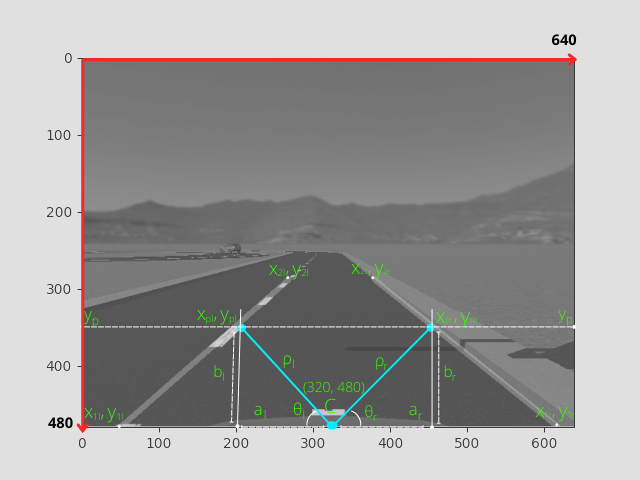
\includegraphics[width=0.75\textwidth]{Figures/Figures_Cap04/avg_polar_lines.png}
    \caption{Geometría de líneas guía del vehículo.}
    \label{fig:avg_polar_lines}
\end{figure}

Una vez que se cuenta con los parámetros de cada una de las rectas desde el centro del vehículo a cada borde del carril es más sencillo calcular las leyes de control. El seguimiento de carril de este trabajo considera cuatro situaciones diferentes en las que podría estar el vehículo.
\begin{enumerate}
    \item Ambas líneas (izquierda y derecha) de los bordes del carril son detectadas indican que el vehículo se encuentra en línea recta.
    \item Solo la línea del borde izquierdo es detectada supone que el vehículo se encuentra en una curva hacía la derecha.
    \item Solo la línea del borde derecho es detectada supone que el vehículo se encuentra en una curva hacía la izquierda.
    \item Ningún borde es detectado indica que el vehículo está fuera de un carril y debe detenerse.
\end{enumerate}

Estas cuatro situaciones son suficientes para que el vehículo pueda determinar la línea con la cual debe guiarse a fin de mantenerse dentro del carril mientras avanza. El seguimiento de carril es logrado usando una ley de control que combina la distancia y el ángulo con respecto al borde del carril. Considerar la figura \ref{fig:línes_desired_lines_detected}, donde las líneas de color verde representan las líneas deseadas si el vehículo se encuentra alineado con los bordes del carril, estas líneas pertenecen a los parámetros $(\rho_{ld}, \theta_{ld})$, $(\rho_{rd}, \theta_{rd})$ para los bordes izquierdo y derecho del carril respectivamente. Líneas en color cyan corresponden a las líneas actualmente observadas de cada borde $(\rho_{l}, \theta_{l})$ y $(\rho_{r}, \theta_{r})$.

\begin{figure}
    \centering
    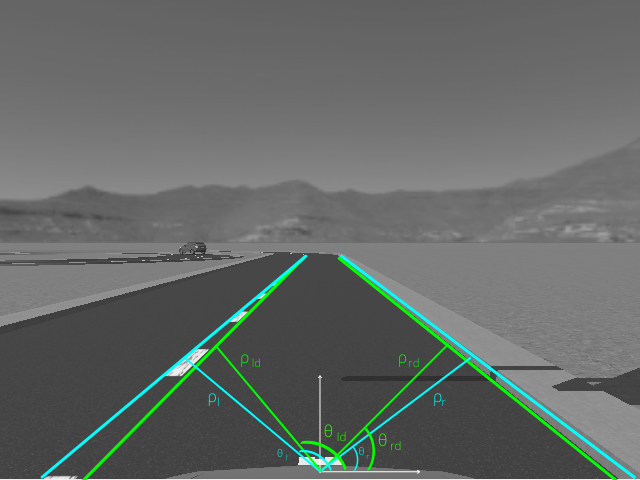
\includegraphics[width=0.75\textwidth]{Figures/Figures_Cap04/lines_control_laws.png}
    \caption{Comparación entre líneas deseadas (verde) y líneas detectadas (cyan).}
    \label{fig:línes_desired_lines_detected}
\end{figure}

La ley de control para movimiento longitudinal del vehículo o velocidad se considera constante en todo momento.
\begin{equation}
    v = C
    \label{eqn:cruise_speed}
\end{equation}

La ley de control en el caso del movimiento lateral o ángulo de dirección es determinado mediante:
\begin{equation}
    \delta = K_\rho e_\rho + K_\theta e_\theta
    \label{eqn:steering_angle}
\end{equation}

Donde $e_\rho$ y $e_\theta$ son errores de distancia y ángulo respectivamente, calculados con las ecuaciones:
\begin{equation}
    e_\rho = \rho_d - \rho_o
    \label{eqn:distance_error}
\end{equation}
\begin{equation}
    e_\theta = \theta_d - \theta_o
    \label{eqn:angle_error}
\end{equation}

Los subíndices $d$ y $o$ en las ecuaciones (\ref{eqn:distance_error})-(\ref{eqn:angle_error}) son etiquetas para ``deseado'' y ``observado'' respectivamente.

Como se mencionó anteriormente dentro del seguimiento del carril se consideran tres casos, las ecuaciones (\ref{eqn:steering_angle})-(\ref{eqn:distance_error})-(\ref{eqn:angle_error}) funcionan bien en los casos donde existen curvas, es decir, cuando solo se detecten bordes del lado izquierdo o bordes del lado derecho. Sin embargo, para seguir el carril en línea recta resulta mejor trabajar con un error promedio de distancia y ángulo en la ecuación (\ref{eqn:steering_angle}) pues ambos bordes del carril se encuentran presentes. Por lo tanto, en este caso las ecuaciones (\ref{eqn:distance_error})-(\ref{eqn:angle_error}) se reescriben de la forma.

\begin{equation}
    e_{\rho_{p}} = \frac{\rho_{l_{d}} - \rho_{l_{o}} + \rho_{r_{d}} - \rho_{r_o}}{2}
    \label{}
\end{equation}
\begin{equation}
    e_{\theta_{p}} = \frac{\theta_{l_{d}} - \theta_{l_{o}} + \theta_{r_{d}} - \theta_{r_{o}}}{2}
    \label{}
\end{equation}

Nuevamente los subíndices $d$ y $o$ son ``deseado'' y ``observado''. Mientras que $p$ es ``promedio'', $r$ y $l$ son \textit{right} y \textit{left} respectivamente.

Entonces la ecuación (\ref{eqn:steering_angle}) queda de la forma:
\begin{equation}
    \delta = K_\rho e_{\rho_{p}} + K_\theta e_{\theta_{p}}
\end{equation}


En cualquiera de los casos anteriores las constantes $K_\rho$ y $K_\theta$ son constantes de sintonización que permiten ajustar el error de distancia y ángulo para precisar el ángulo de dirección que mantendrá el vehículo en cada caso. Estas constantes son obtenidas de manera experimental porque al ser un ambiente simulado no se pueden tener medidas reales de estos parámetros. Una manera fácil de obtener los valores numéricos esperados para $(\rho_{l_{d}}, \theta_{l_{d}})$ y $(\rho_{r_{d}}, \theta_{r_{d}})$ es obtenerlos desde el principio de la simulación con el supuesto de que el vehículo se encuentra bien centrado dentro del carril. Cabe resaltar que se pretenden giros suaves del vehículo para mantener un comportamiento lo más natural y parecido en comparación como lo realizan conductores al frente del volante, bajo estas condiciones el ángulo de dirección disminuye o aumenta en pasos de $1^\circ$.

Con el cálculo de estas ecuaciones, el ángulo de dirección del vehículo siempre se mantiene en un rango seguro para que no salga del carril, mientras que la velocidad es constante en todo momento. Con los cuatro casos anteriores en cuanto a detección de las líneas que conforman el carril se determina que el vehículo puede manejar en situaciones reales guiándose con los bordes del carril. Además, con el objetivo de mantener la integridad del vehículo en líneas curvas se considera una velocidad menor respecto a líneas rectas donde la velocidad es mayor. Sin embargo, en un caso extremo donde el vehículo no sea capaz de detectar un carril por diferentes situaciones la mejor opción es dejar de avanzar, es decir, se considera velocidad $= 0$ y ángulo de dirección $=0$.

Finalmente y con el propósito de demostrar que las operaciones de detección y seguimiento de carril corresponden al resultado esperado se presenta \ref{fig:lane_detect_tracking} como conjunto de imágenes que ilustran cada uno de los escenarios esperados.

\begin{figure}[h]
    \centering
    \begin{subfigure}[b]{0.2\textwidth}
         \centering
         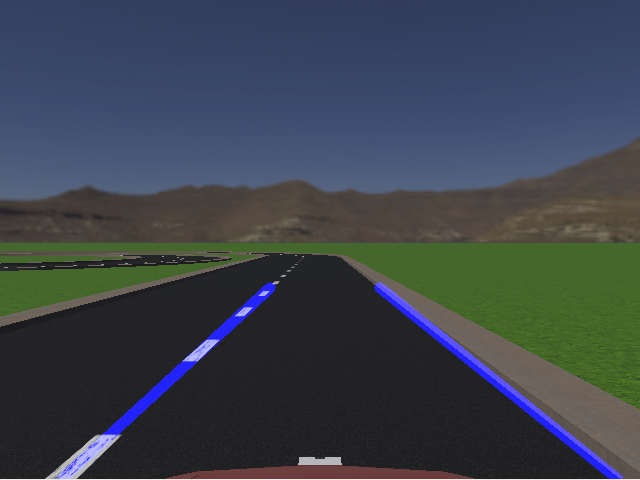
\includegraphics[width=\textwidth]{Figures/Figures_Cap04/both_bordes_detected.png}
         \caption{Ambos bordes}
         \label{fig:both_borders_detected}
    \end{subfigure}
    \hfill
    \begin{subfigure}[b]{0.2\textwidth}
         \centering
         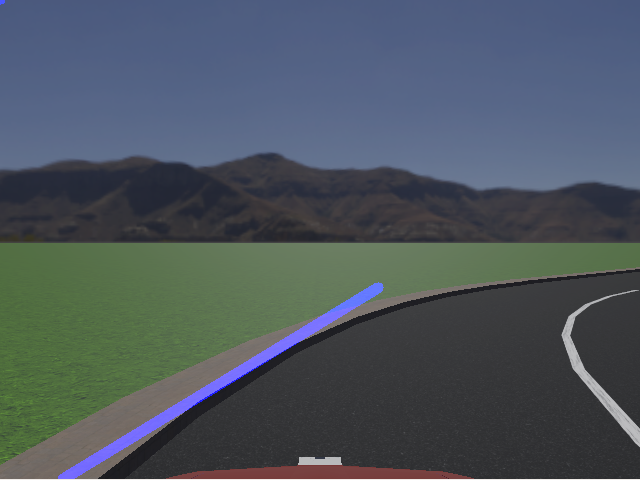
\includegraphics[width=\textwidth]{Figures/Figures_Cap04/left_border_detected.png}
         \caption{Solo borde izquierdo}
         \label{fig:left_border_detected}
     \end{subfigure}
     \hfill
     \begin{subfigure}[b]{0.2\textwidth}
         \centering
         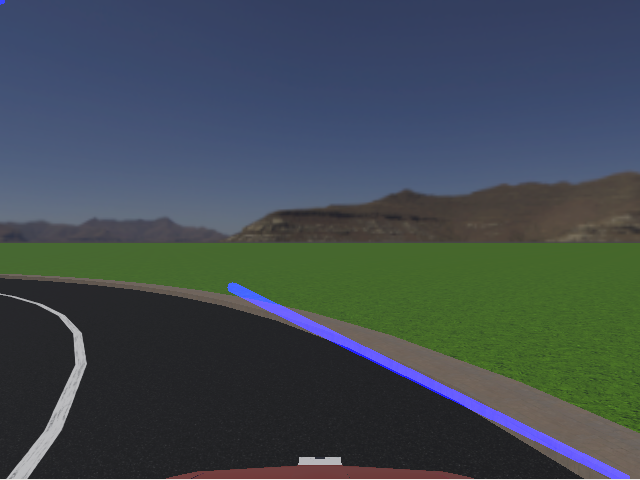
\includegraphics[width=\textwidth]{Figures/Figures_Cap04/right_border_detected.png}
         \caption{Solo borde derecho}
         \label{fig:right_border_detected}
     \end{subfigure}
     \hfill
     \begin{subfigure}[b]{0.2\textwidth}
         \centering
         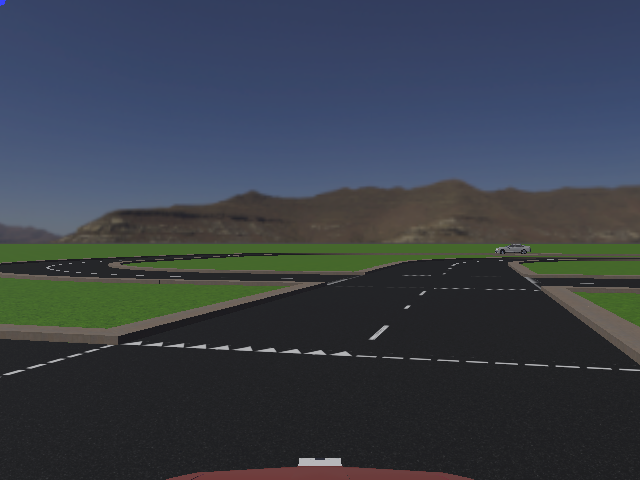
\includegraphics[width=\textwidth]{Figures/Figures_Cap04/no_borders_detected.png}
         \caption{Sin bordes detectados}
         \label{fig:no_edge_detected}
     \end{subfigure}
     
    \caption{Casos considerados según bordes detectados en el seguimiento de carril.}
    \label{fig:lane_detect_tracking}
\end{figure}

En \ref{fig:both_borders_detected} ambos bordes son detectados e indica movimiento en línea recta, las figuras \ref{fig:left_border_detected} y \ref{fig:right_border_detected} corresponden a los casos de curva hacia la derecha y curva hacia la izquierda respectivamente. En curvas a la izquierda debe de prevalecer un ángulo de dirección negativo y en el caso de curvas a la derecha el ángulo tiende a ser positivo. \ref{fig:no_edge_detected} representa una situación donde ningún borde de carril es detectado y la mejor opción es frenar el movimiento. Con este conjunto de imágenes se comprueba el correcto funcionamiento de la detección de carril y seguimiento de carril con las leyes de control diseñadas.
\newpage

%CONCLUSIONES DEL CAPÍTULO
Este capítulo concluye con la implementación de las herramientas matemáticas de detector de bordes de Canny en una imagen y transformada Hough para detección de líneas rectas. Se demostró que se puede desarrollar un sistema de visión artificial que permita el reconocimiento de carriles en la escena a partir de imágenes RGB. Además, se diseñó e implementó un control para establecer operaciones tácticas de movimiento longitudinal y lateral que se ven involucradas en el seguimiento de carril. Con ello, el vehículo fue capaz de recorrer en su totalidad el circuito propuesto en la sección \ref{sec:el_ambiente_de_simulación}, sin obstáculos. 

Sin embargo, en esta sección solo se contemplan situaciones controladas donde no existe ningún otro vehículo a parte del autónomo, lo cual es muy poco probable en el mundo real. De esta manera, el único inconveniente que se puede presentar es que el vehículo deje de detectar carriles para guiar su trayecto. En los siguientes capítulos se aspira a añadir más características al ambiente simulado que sumen en dificultad para la navegación autónoma del vehículo, como es el caso de nuevos vehículos para la detección obstáculos, evasión y seguimiento de vehículos.
\chapter{Detección de obstáculos} \label{cap:detección_de_obstáculos}
% BREVE DESCRIPCIÓN DEL CONTENIDO DE ESTE CAPÍTULO
Este capítulo busca añadir mayor detalle a la caracterización del ambiente, en específico detectar objetos potencialmente peligrosos para el vehículo autónomo. Primero, en la sección \ref{sec:introducción_a_la_detección_de_ obstáculos}, se exponen aspectos básicos acerca de como un conductor puede detectar objetos en el camino. La sección, \ref{sec:algoritmos_de_agrupamiento} es una descripción de las categorías y características de los algoritmos de agrupación, mientras que la subsección, \ref{sub:ejemplo_para_obtener_una nube_de_puntos_con_ROS} es un ejemplo de como procesar una nube de puntos con ROS. Enseguida, la sección \ref{sec:el_algoritmo_K-medias} y subsección \ref{sub:ejemplo_de_implementación_del_algoritmo_K-medias} se enfocan en la definición teórica e implementación en código del algoritmo \textit{k-means} respectivamente. A continuación, la sección \ref{sec:empatado} habla acerca de la importancia de implementar un algoritmo de empatado. Finalmente, en \ref{sec:el_filtro_de_Kalman} se expone teóricamente el concepto de filtro de Kalman y \ref{sub:el_filtro_de_Kalman_extendido} su versión extendida, además, la subsección \ref{sub:estimación_de_posición_y_velocidad_con_el_filtro_de_kalman_extendido}, es un ejemplo de diseño e implementación de un filtro de Kalman para seguimiento de objetos.

Es importante mencionar que la implementación de códigos de este capítulo resulta en una combinación de lenguajes de programación C++ y Python, esta decisión se justifica y explica en las secciones correspondientes. Al finalizar este capítulo se muestran los resultados de las implementaciones aquí desarrolladas y en adición con la labor del seguimiento de carriles previamente diseñada, el vehículo autónomo no tripulado contará con un sistema más robusto que le permitirá tener una mejor percepción del ambiente.

\section{Introducción a la detección de obstáculos} \label{sec:introducción_a_la_detección_de_ obstáculos}

Los humanos pueden evitar obstáculos en el ambiente vehicular mientras manejan haciendo uso de los sentidos de la vista y oído. Con ellos, pueden percibir el ambiente y conocer si algún vehículo u obstáculo se encuentra al frente, por detrás o en los laterales. Es decir, conocen aunque con poca exactitud la posición de los obstáculos. Además, mediante la posición determinan que tan rápido avanzar para no chocar al frente, cuando comenzar a frenar en caso necesario e incluso fijar el ángulo de dirección en un rango estable para no chocar a los costados. Sin embargo, un vehículo autónomo no cuenta con un sistema que le permita realizar estas tareas de manera natural pues solo está instrumentado con sensores que le permiten conocer el ambiente. Con ayuda de algoritmos e instrumentos matemáticos y en combinación con información de sensores es posible simular estos comportamientos innatos para el ser humano.

El objetivo de este capítulo es contar con instrumentos que permitan determinar una situación donde intervenga la evasión de obstáculos a partir de dos tareas principales. En la sección anterior se mencionó la nula presencia de vehículos dentro del circuito de pruebas, ya es bien sabido que un ambiente vial cotidiano existen diversos objetos que podrían provocar colisiones. En específico, se buscan evitar accidentes del vehículo autónomo con otros vehículos dentro del circuito. Antes de definir una situación de evasión de objetos se requieren dos fases:
\begin{itemize}
    \item Detección de objetos
    \item Seguimiento de objetos
\end{itemize}
El objetivo de la detección es encontrar aquellos objetos potencialmente peligrosos para provocar cualquier tipo de accidente con el vehículo no tripulado, un escenario sencillo para navegación autónoma es usar las líneas del carril como guía dentro de un circuito cerrado. Sin embargo, en la búsqueda de situaciones más reales es importante considerar vehículos u otro tipo de objetos con diferentes tamaños, colores y obviamente posiciones distintas. La detección de objetos debe clasificar aquellos objetos que se encuentren dentro de la carretera pero en especial que impliquen un problema en la navegación del vehículo autónomo.

Una herramienta tecnológica en robótica que ayuda a ubicar objetos son los sensores láser. Como se mencionó en la subsección \ref{sub:sensores} un sensor LIDAR otorga puntos pertenecientes a una superficie. Este conjunto de puntos también conocido como nube de puntos no provee la información necesaria para decidir que objetos resultan un riesgo para el vehículo, por esta razón es necesario agrupar la nube de puntos en conjuntos que describan un objeto potencialmente peligroso y posteriormente determinar su posición. Las técnicas de agrupación tienen la capacidad de cumplir esta labor además, pueden trabajar con conjuntos grandes en tamaño para agruparlos en pequeños grupos de acuerdo a sus características. Dentro de la gran variedad de algoritmos de agrupación se encuentra el algoritmo \textit{k-means} que se caracteriza por agrupar bancos de datos en base a la cercanía (distancia) que existe entre ellos. 

Por otro lado, se entiende que los vehículos pueden desplazarse principalmente de manera vertical y en menor medida horizontalmente o por alguna razón pueden permanecer estáticos. Es evidente que los vehículos estáticos tienen velocidad $v = 0$,  mientras que la posición puede ser cualquier punto en el espacio pero constante. Sin embargo, en el caso contrario cuando la velocidad $v \neq 0$, la posición es distinta en cada momento y es proporcional a la velocidad que presente el vehículo. Este comportamiento implica la necesidad de predecir de alguna manera la velocidad y posición de vehículos estáticos y en movimiento. El seguimiento de vehículos tiene el objetivo de cumplir esta meta con ayuda de un instrumento matemático conocido como filtro de Kalman, el cual permite predecir estados futuros de un sistema dinámico.

Cada una de estas fases tienen desarrollos distintos, los cuales son:
\begin{itemize}
    \item Detección de objetos
        \begin{enumerate}
            \item Obtener la nube de puntos otorgada por el sensor LIDAR.
            \item Agrupar la nube de puntos.
            \item Obtener la posición de cada objeto detectado.
        \end{enumerate}
    \item Seguimiento de objetos
    \begin{enumerate}
        \item Diseñar un sistema dinámico que involucre posición y velocidad.
        \item Estimar posiciones y velocidades futuras de cada objeto.
    \end{enumerate}
\end{itemize}

La combinación de detectar y seguir obstáculos es esencial para iniciar con la tarea específica de evasión de obstáculos. 

\section{Algoritmos de agrupamiento} \label{sec:algoritmos_de_agrupamiento}

Existe una gran variedad de algoritmos de agrupación y por ello, resulta complicado hacer una clasificación exacta de estos métodos porque algunas categorías podrían superponerse con otras, de modo que, un algoritmo puede poseer características de una o varías categorías. No obstante, es de mucha utilidad crear una organización relativa para los métodos de agrupamiento existentes. Los principales algoritmos de agrupación pueden ser clasificados en las siguientes categorías \cite{han2011data}.

\begin{enumerate}
    \item \textbf{Métodos de división:} Centran su funcionamiento en el calculo de distancias por ejemplo, distancia de \textit{Manhattan} o distancia Euclidiana (\ref{eqn:euclidian_distance}). Dado un conjunto de $n$ objetos, un método de división construye $k$ divisiones. Cada división representa un \textit{cluster} o grupo con $k \leq n$. Este tipo de algoritmos agrupan los datos en $k$ \textit{clusters} y cada \textit{cluster} contiene al menos un objeto.
    
    Sea $k$ el número de divisiones a construir, el método de división crea una división inicial. Después usa una técnica de reubicación iterativa que busca mejorar el agrupamiento moviendo los objetos de un grupo a otro. El criterio general para asignar objetos en un grupo es que tan cerca o relacionados están los objetos de un grupo, mientras que objetos en diferentes \textit{clusters} se mantienen lejanos o son muy diferentes. \textit{k-means} y \textit{k-medoids} son ejemplos de esta técnica de agrupación. Estos métodos funcionan bien para agrupar conjuntos con formas esféricas en conglomerados de tamaño pequeño o mediano. Para formar grupos con formas complejas y con conjuntos de mayor tamaño, es necesario mejorar o buscar otros métodos.
    
    \item \textbf{ Métodos jerárquicos:} Un método jerárquico se caracteriza por crear una descomposición jerárquica del conjunto de datos inicial en objetos de datos. Los métodos jerárquicos se pueden clasificar según la estrategia que implementan, ya sea aglomerativa o divisiva. También conocido como enfoque de abajo hacia arriba, el método de aglomeración comienza formando un grupo por cada objeto para después fusionar los objetos o grupos cercanos entre sí, hasta que todos los grupos forman uno solo o bien se cumple una condición de paro. El enfoque divisivo, igualmente llamado enfoque de arriba hacia abajo, inicia con todos los objetos dentro de un grupo. Luego, un grupo se divide en grupos más pequeños por cada iteración hasta que cada objeto está en un grupo o una condición de paro se cumpla.
    
    Los métodos jerárquicos cuentan con una condición de rigidez porque una vez que un paso de combinación o división es realizado no se puede anular. Sin embargo, esta desventaja es aprovechada por provocar menores costos de cálculo al no tener preocupación por un número de diferentes combinaciones. Una desventaja más de estas técnicas radica en que no pueden corregir decisiones erróneas.
    
    \item \textbf{ Métodos basados en densidad:} Uno de las principales inconvenientes de los métodos de agrupación por división es que solo funcionan bien para encontrar formas esféricas mientras que estructuras arbitrarías resulta una tarea difícil. Otros métodos de agrupación han sido desarrollados bajo la noción de densidad (número de objetos o puntos de datos). Su idea general consiste en incrementar un determinado grupo siempre y cuando la densidad de una vecindad exceda un umbral. Es decir, para cada punto contenido en un grupo, la vecindad debe de contener un mínimo de puntos.
    
    Este tipo de métodos son útiles para reducir ruido en valores atípicos provocados por lecturas de sensores además de descubrir grupos con formas arbitrarias.
    
    \item \textbf{Métodos basados en cuadrículas:} Los métodos basados en cuadrículas se pueden integrar con distintos métodos de agrupación, como los métodos basados en densidad y los métodos jerárquicos, a menudo resulta eficiente el uso de cuadrículas en muchas aplicaciones de la minería de datos. El agrupamiento por cuadrículas cuantifica el espacio de un objeto en un número finito de celdas que forman una estructura de cuadrícula, todas las operaciones de agrupación son realizadas dentro de la cuadrícula, es decir, el espacio cuantificado. La principal ventaja de este método es el bajo coste computacional y rápido tiempo de procesamiento, pues por lo general es independiente del número de datos a agrupar y solo depende de la cantidad de celdas en cada dimensión dentro del espacio cuantificado.
\end{enumerate}

\begin{equation}
    d_E(P_1, P_2) = \sqrt{(x_1 - x_2)^2 - (y_1 - y_2)^2}
    \label{eqn:euclidian_distance}
\end{equation}

Algunos de los algoritmos de agrupación integran ideas de distintos métodos, por lo que en ocasiones es difícil colocar un algoritmo dentro de una categoría específica. Además, algunas aplicaciones llegan a presentar criterios que requieren de más de un método de agrupación. El cuadro \ref{tab:clustering_methods} muestra las principales características las clasificaciones antes descritas. En este trabajo se utilizará un método de agrupación por división, ver sección \ref{sec:el_algoritmo_K-medias}.
\begin{table}[t]
    \begin{center}
    \begin{tabular}{| l | l |}
    \hline
    Método & Características Principales \\ \hline
    De división & Basado en distancia \\ & Efectivo en conjuntos pequeños y medianos \\ & Utiliza la media o medoides para representar \\ & el centro de un \textit{cluster}  \\ \hline
    Jerárquico & Puede incorporar otras técnicas \\ & El agrupamiento es una descomposición \\ & jerárquica \\ & No corrige después de una combinación o \\ & división \\ \hline
    Basado en densidad  & Encuentran formas arbitrarias \\ & Filtran valores atípicos  \\ & Cada punto debe tener un mínimo de \\ & puntos dentro de su vecindad \\ \hline
    Basado en cuadrículas & Una cuadrícula es la estructura de datos \\ & Es más rápido que otros métodos \\ \hline
\end{tabular}
    \end{center}
    \caption{Clasificaciones de algoritmos de agrupamiento y sus principales características.}
    \label{tab:clustering_methods}
\end{table}

\subsection{Ejemplo para obtener una nube de puntos con \textit{ROS}} \label{sub:ejemplo_para_obtener_una nube_de_puntos_con_ROS}

El primer paso en la detección de objetos es contar con un instrumento que permita caracterizar el ambiente que rodea al vehículo de pruebas. Webots tiene la facilidad de simular diferentes sensores que instrumentan el vehículo de forma independiente, de manera similar a la cámara existe un nodo específico en el simulador para seleccionar un sensor LIDAR de un amplío catálogo que incluye algunas de las marcas y modelos más comerciales como: Velodyne, SICK, Hokuyo y Robotis. Sin embargo, Webots también ofrece la posibilidad de caracterizar un nodo LIDAR con las características únicas y necesarias para propósitos específicos. Está flexibilidad es una gran ventaja porque permite especificar los parámetros requeridos que mejor se ajusten a la aplicación en turno.

De este modo, los principales parámetros requeridos del sensor LIDAR a usar son:
\begin{itemize}
    \item \textbf{Campo de visión horizontal:} $2\pi = 360^{\circ}$
    \item \textbf{Resolución horizontal:} 1024 puntos por capa
    \item \textbf{Campo de visión vertical:} $0.3^{\circ}$, ángulo entre primera y última capa
    \item \textbf{Número de capas:} 16
    \item \textbf{Rango máximo:} 30[m]
\end{itemize}

Otra razón para usar un sensor LIDAR convencional y con parámetros específicos es qué se tiene un mayor control sobre el número de puntos otorgados por el sensor, pues esta característica es de vital importancia para el desempeño de un algoritmo de clusterización.

De manera similar a la imagen de la cámara descrito en el capítulo \ref{cap:seguimiento_de_carriles}, pero con las diferencias necesarias se pretende obtener la información del sensor LIDAR, en específico la nube de puntos. El proceso para obtener la nube de puntos del sensor requiere un mensaje tipo \textit{PointCloud2}, las parámetros más importantes de este mensaje incluyen: alto y ancho de la nube de puntos, tamaño de una fila y de cada punto en bytes además de la propia nube de puntos en cada momento, etc. Cada uno de los parámetros requeridos por el mensaje \textit{PointCloud2} contienen los valores recomendados en las documentaciones de Webots y \textit{ROS}, el parámetro más importante de este mensaje es \textit{data} y debe de contener una estructura del tipo \textit{bytearray} por recomendación de la propia documentación, ya que usar una lista convencional tiene la desventaja de ser más lento entre más puntos contenga la nube de puntos. El controlador principal del vehículo de pruebas desarrollado en Python propone el siguiente código para este efecto.

\hfill
\begin{lstlisting}[language=Python]
# INIT LIDAR
lidar = Lidar('lidar')          
lidar.enable(TIME_STEP)
lidar.enablePointCloud()

# POINT CLOUD2 MESSAGE 
msg_point_cloud = PointCloud2()
msg_point_cloud.header.stamp = rospy.Time.now()
msg_point_cloud.header.frame_id = 'lidar_link'  
msg_point_cloud.height = 1
msg_point_cloud.width = lidar.getNumberOfPoints()
msg_point_cloud.point_step = 20
msg_point_cloud.row_step = 20 * lidar.getNumberOfPoints()
msg_point_cloud.is_dense = False
msg_point_cloud.fields = [
    PointField(name = 'x', offset = 0, datatype = PointField.FLOAT32, count = 1),
    PointField(name = 'y', offset = 4, datatype = PointField.FLOAT32, count = 1),
    PointField(name = 'z', offset = 8, datatype = PointField.FLOAT32, count = 1),
]
msg_point_cloud.is_bigendian = False
msg_point_cloud.data = lidar.getPointCloud(data_type='buffer')       
\end{lstlisting}
\hfill

Con el mensaje \textit{PointCloud2} se define un tópico que publica el contenido del mensaje, posteriormente se debe agrupar la nube puntos con un algoritmo de agrupación, también se usa el mensaje para tener una visualización de la nube de puntos a través del visualizador RViz de \textit{ROS}. Este paquete tiene la particularidad de recibir múltiples mensajes de sensores disponibles en \textit{ROS} y realizar visualizaciones 3D de estos. 

La imagen \ref{fig:pc_webots} muestra la nube de puntos vista desde el simulador. A manera de respaldar el resultado del código anterior se presenta la misma nube de puntos pero en el visualizador RViz, ver \ref{fig:pc_rviz}.
\begin{figure}[h]
    \centering
    \begin{subfigure}[b]{0.4\textwidth}
         \centering
         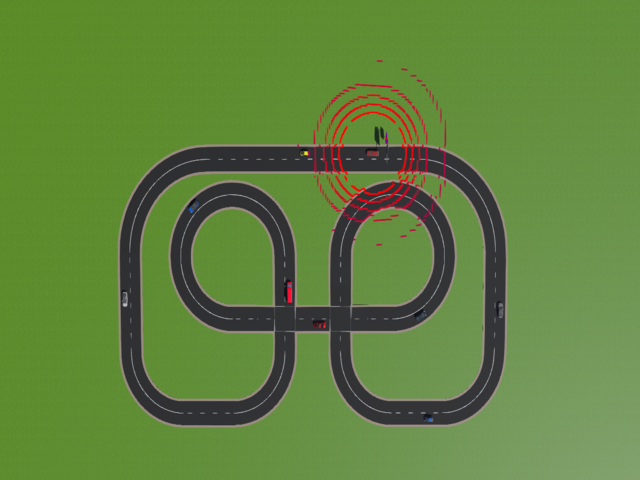
\includegraphics[width=\textwidth]{Figures/Figures_Cap05/pc_webots.png}
         \caption{Nube de puntos en Webots.}
         \label{fig:pc_webots}
    \end{subfigure}
    \hfill
    \begin{subfigure}[b]{0.4\textwidth}
         \centering
         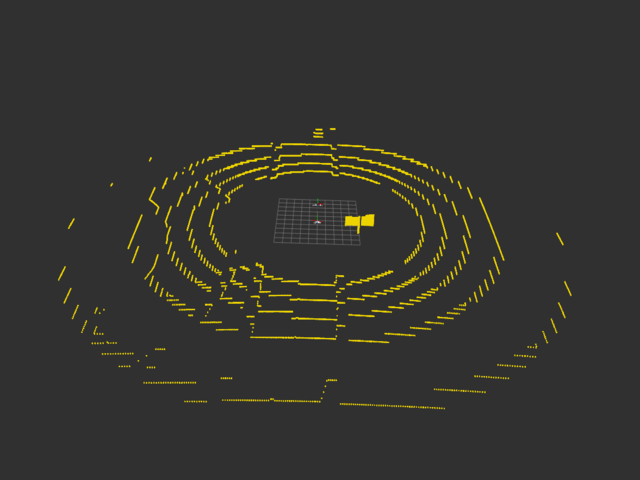
\includegraphics[width=\textwidth]{Figures/Figures_Cap05/pc_rviz.png}
         \caption{Nube de puntos en Rviz.}
         \label{fig:pc_rviz}
     \end{subfigure}
     
    \caption{Nube de puntos en Webots y Rviz.}
    \label{fig:pc_webots_rviz}
\end{figure}

\section{El algoritmo K-medias} \label{sec:el_algoritmo_K-medias}

La versión más simple y fundamental para el análisis de grupos es la división, organiza objetos de un conjunto en varios grupos o \textit{clusters}. Para mantener la especificación del problema, se entiende que el número de \textit{clusters} iniciales se proporciona con conocimiento previo ya que este parámetro es el punto de partida en cualquier método de agrupación por división.

Sea \textit{D} un conjunto de datos, con \textit{n} objetos, y \textit{k}, el número de grupos por formar, un algoritmo de agrupación por división ordena los objetos en \textit{k} particiones con $k \leq n$, donde cada partición representa un grupo. Los \textit{clusters} se forman a partir de una función de disimilitud basada en distancia como criterio, objetos contenidos en un \textit{cluster} son similares entre sí pero diferentes a los objetos de otros \textit{clusters}. Dado un conjunto \textit{D} con \textit{n} objetos en el espacio euclidiano. Los métodos de división distribuyen los \textit{n} datos de \textit{D} en \textit{k} grupos $C_1, C_2, C_3,..., C_k$. Se utiliza una función objetivo para evaluar la partición de la división. Es decir, la función objetivo busca una alta similitud dentro de un grupo y una baja similitud con grupos externos.

El algoritmo \textit{k-means} es una técnica de división basada en centroide, dicho de otra manera utiliza el centroide $c$ para representar un grupo $C$. Teóricamente, el centroide de un \textit{cluster} es su punto central. La definición de centroide puede ser de distintas maneras, como la media o medoide de los puntos u objetos asignados al grupo.

La diferencia entre un objeto $p_i \in C_i$ y su centroide $c_i$ se mide como $d(p_i, c_i)$, donde $d$ es la distancia euclidiana entre dos puntos en $[x, y]$. La calidad del \textit{cluster} $C_i$ se puede medir como la variación del grupo, que es la suma del error cuadrático entre todos los objetos $p_i$ en $C_i$ y el centroide $c_i$, como:
\begin{equation}
    E = \sum_{i=1}^{k}\sum_{p\in{C_i}}d(p_i, c_i)^2
\end{equation}

donde \textit{E} es la suma del error cuadrático de todos los puntos en el conjunto de datos, $p_i$ es un punto en el espacio que representa un objeto; y $c_i$ es el centroide del \textit{cluster} $C_i$. Dicho de otra manera, la distancia desde un punto hacia el centro de su grupo se eleva al cuadrado y las distancias se suman. El propósito de esta función objetivo es hacer que los \textit{k} \textit{clusters} resultantes sean lo más separados y compactos posibles, \textit{k-means} establece el centroide de un \textit{cluster} como el valor medio de los puntos que contiene. 

Al comenzar, \textit{k-means} selecciona aleatoriamente \textit{k} objetos de \textit{D}, cada uno de estos representa inicialmente un centro o media de \textit{cluster}. Todos y cada uno de los objetos $p_i$ restantes se reasignan al grupo que más sean similares en función de la distancia euclidiana que existe entre el punto $p_i$ y la media de grupo $c_i$. En otras palabras, cada objeto $p_i$ se une al grupo $C_i$ más cercano y $c_i$ representa la media de todos los objetos que contiene $C_i$. Después, el algoritmo mejora iterativamente la variación dentro del grupo calculando una nueva media de los objetos asignados al \textit{cluster} en la iteración anterior. En breve, todos los objetos se reasignan utilizando el valor medio de cada \textit{cluster} como el nuevo centroide $c_i$ de $C_i$. El proceso iterativo se repite hasta que la asignación es estable, es decir, los grupos formados en la ronda actual son los mismos que se formaron en la ronda anterior. Dicho de otro modo, la diferencia entre $c_i$ anterior y $c_i$ actual es mínima. El algoritmo \ref{alg:k-means} describe este proceso.
\begin{algorithm}
    \begin{algorithmic}[0]
        \REQUIRE $k:$ Número de \textit{clusters} \\ \parindent=12.5mm $D:$ Conjunto de datos con $n$ objetos
        \ENSURE $k$ centroides
        \STATE Obtener centroides iniciales $C = \{c_0, c_1, .... , c_k\}$ con $k$ objetos de $D$
        \FORALL{$p$ en $D$}
            \STATE Calcular $d(p_i, c_i) = \sqrt{(p_{i_{x}} - c_{i_{x}})^2 + (p_{i_{y}} - c_{i_{y}})^2 (p_{i_{z}} - c_{i_{z}})^2}$
            \STATE Añadir $p_i$ al \textit{cluster} $c_i$ más cercano
        \ENDFOR
        \STATE Obtener nuevos centroides $C_n = \{\bar{c_0}, \bar{c_1}, .... , \bar{c_k}\}$
        \STATE Calcular $\Sigma d(C, C_n)$.
        \WHILE{$\Sigma d(C, C_n) > tolerancia$}
            \STATE Actualizar $C$ $\leftarrow$ $C_n$
            \STATE Reagrupar $p_i$ en $c_i$
            \STATE Recalcular $C_n = \{\bar{c_0}, \bar{c_1}, .... , \bar{c_k}\}$
            \STATE Recalcular $\Sigma d(C, C_n)$
        \ENDWHILE
        \RETURN $k$ centroides
    \end{algorithmic} 
  
    \caption{Algoritmo \textit{K-means}.}
    \label{alg:k-means}
\end{algorithm}

Sin embargo, no se garantiza que \textit{k-means} converja a un óptimo global y en muchos de los casos termina en un óptimo local. Por otro lado, el resultado de la agrupación puede depender de la selección aleatoria inicial de centroides. En la práctica, para obtener mejores resultados es común ejecutar el algoritmo \textit{n} veces con diferentes centroides iniciales. La complejidad de \textit{k-means} es de $O(nkt)$; donde \textit{n} es total de objetos, \textit{k} es el número de \textit{clusters} a formar y \textit{t} el número de iteraciones. Por lo tanto, este método es relativamente escalable para grandes conjuntos de datos.

El método \textit{k-means} no resulta adecuado para descubrir formas arbitrarias. Además, es sensible al ruido y a datos atípicos pues pueden influir sustancialmente en el valor medio. Existen diferentes variantes del método \textit{k-means} que pueden diferir en la selección de los \textit{k} \textit{clusters} iniciales, el cálculo de la disimilitud y estrategias para calcular la media de los \textit{clusters}.

\subsection{Ejemplo de implementación del algoritmo K-medias} \label{sub:ejemplo_de_implementación_del_algoritmo_K-medias}

El segundo paso en la detección de objetos es implementar un algoritmo de agrupación, como se mencionó anteriormente el algoritmo \textit{k-means} es el elegido para agrupar la nube de puntos del sensor LIDAR y lograr la detección de objetos, en específico vehículos. Debido a que el sensor LIDAR está situado en la parte superior del vehículo, ver \ref{fig:webots_car}, es importante delimitar el área donde existan puntos de interés en la búsqueda de objetos potencialmente peligrosos. En breve se enuncia el proceso para agrupar la nube de puntos.   
\begin{enumerate}
    \item Eliminar puntos que pertenezcan al suelo del escenario.
    \item Definir el número de \textit{clusters} iniciales que serán los encargados de identificar obstáculos.
    \item Aplicar \textit{k-means} al conjunto de puntos previamente filtrado.
\end{enumerate}

En un primer intento por implementar el algoritmo \textit{k-means} se usó Python como lenguaje de programación donde se logró el objetivo de obtener los centroides que indican la posición de cada objeto contenido en la escena. Sin embargo, se presentaron algunos inconvenientes en los resultados finales, por ejemplo: 
\begin{itemize}
    \item La posición de los centroides no es constante con la posición de los objetos. Es decir, la posición de los centroides  varía en cada momento aún cuando los objetos permanecen estáticos.
    \item La velocidad del algoritmo incrementa conforme crece el tamaño de la nube de puntos.
\end{itemize}

Para lidiar con estos inconvenientes se decide hacer una nueva implementación del algoritmo \textit{k-means} pero ahora en lenguaje de programación C++ con el fin de tener más control en cada una de las operaciones que involucra el algoritmo además de disminuir el tiempo de procesamiento del mismo.

Para completar el primer requisito del agrupamiento es necesario filtrar la nube de puntos y eliminar puntos pertenecientes al suelo. Es difícil tener una medición exacta que permita delimitar la altura que existe desde el suelo hasta la posición del sensor LIDAR. Debido a esto mediante experimentación se llega al valor de $-1.5[m]$ en el eje $y$ que representa la altura en el sistema coordenado, este valor en $y$ es un umbral que delimita puntos que forman el suelo y puntos que no son parte de él. Es decir, todos los puntos $ y<-1.5$ son despreciados, además se eliminan puntos con valor $inf$ o $NaN$ de la nube de puntos para evitar posibles errores en operaciones posteriores del algoritmo \textit{k-means}. 

En breve se ejemplifica la implementación en código, donde las líneas 2 y 3 muestran las condiciones para eliminar puntos $inf$ y suprimir puntos perteneciente al suelo respectivamente.

\hfill
\begin{lstlisting}[language=C]
void objectDetectCallback(const sensor_msgs::PointCloud2::ConstPtr& msg){
    if( (isinf(x) or isinf(y) or isinf(z)) != true){
        if( y > -1.5 ){
            std::vector<double> point = {x, y, z};
            point_cloud.push_back(point);
        }
    }
}
\end{lstlisting}
\hfill

Definir el número de \textit{clusters} considerados para el algoritmo \textit{k-means} es una ardua tarea en esta aplicación, pues el propósito general es detectar autos y en un ambiente vial existen múltiples situaciones con un número diferente de vehículos en cada situación, como consecuencia de este hecho no se puede definir a priori la cantidad de grupos iniciales que mejor se ajuste a cada una de las situaciones, porque existen una infinidad de casos. Aunque el método del codo o \textit{elbow-method} del algoritmo \textit{k-means} es una herramienta de utilidad que funciona en otro tipo aplicaciones pero, para este caso en particular resulta costoso en tiempo de procesamiento debido a que la nube de puntos cambia mientras el vehículo se desplaza vertical u horizontalmente.

Sin embargo, uno de los propósitos de este trabajo es probar cada uno de los algoritmos bajo un ambiente supervisado y controlado, tal y como se hizo con el circuito de prueba para detección y seguimiento de carril donde el vehículo de pruebas está dentro de un circuito cerrado también se añade un número invariable de vehículos con el objetivo de realizar pruebas en la detección de objetos de manera controlada.  Siguiendo este enfoque se pretende añadir un máximo de 5 diferentes vehículos con distintas posiciones en el circuito de pruebas, por lo tanto el número mínimo de \textit{clusters} iniciales debe de ser $\geq 5$.
\newpage

Con los dos pasos realizados previamente se puede comenzar la implementación del algoritmo \textit{k-means} para agrupar la nube de puntos, como se mencionó anteriormente la implementación en código de este algoritmo es en lenguaje C++ por razones ya explicadas, la implementación corresponde directamente al algoritmo \ref{alg:k-means} y se tienen en cuenta las siguientes consideraciones.
\begin{enumerate}
    \item La agrupación de puntos se define a través de la cercanía que existe entre ellos.
    \item El número y posición de los \textit{clusters} iniciales es definido antes de iniciar el agrupamiento.
    \item La cercanía entre puntos es calculada con distancia euclidiana.
    \item Si un grupo no contiene puntos entonces es ignorado.
    \item Si dos centroides se encuentran a distancia mínima se obtiene el promedio de ambos que resulta en uno solo.
    \item La condición de paro del algoritmo es el cambio mínimo de posición de los centroides o cuando se exceda un máximo de intentos.
\end{enumerate}

\begin{lstlisting}[language=C]
/* KMEANS FUNCTION */
std::vector<std::vector<double>> kmeans(std::vector<std::vector<double>> point_cloud){

    new_centroids = calulate_centroids(point_cloud, initial_centroids);        
    total_distance = compare_centroids(new_centroids, initial_centroids);      

    while (total_distance > tol && attemps < max_attemps){
        std::vector<std::vector<double>> centroids(new_centroids); 
        new_centroids = calulate_centroids(point_cloud, centroids); 
        total_distance = compare_centroids(new_centroids, centroids);
        attemps += 1;
    }
    return new_centroids;                                            
}
\end{lstlisting}
\hfill

La función \textit{kmeans} del código anterior recibe como parámetro una nube puntos y el valor de retorno es el conjunto de centroides calculados, es decir, la posición media de cada uno de los grupos formados por el algoritmo.

Las líneas más importantes del código anterior son explicadas a continuación:
\begin{itemize}
    \item La línea 4 efectúa el agrupamiento para cada punto de la nube y calcula la media de cada centroide por medio de la función \textit{calculate\_centroids()}. Donde el primer parámetro es la nube de puntos y el segundo parámetro corresponde al conjunto de centroides iniciales previamente establecidos.
    \item La línea 5 realiza el calculo de distancia euclidiana total entre centroides actuales e iniciales.
    \item A partir de la línea 7 se inicia un ciclo para repetir el agrupamiento hasta que se cumpla una de las condiciones de paro.
    \item La línea 8 realiza una copia los nuevos centroides para efectuar el siguiente calculo con el valor actualizado. Mientras que 9 y 10 realizan agrupamiento y calculo de distancia entre centroides respectivamente.
\end{itemize}

Al finalizar este proceso se obtiene como resultado un conjunto de centroides que corresponden a la posición media de los grupos formados por el algoritmo de agrupación. La posición de cada centroide se expresa en coordenadas cartesianas en un espacio de tres dimensiones $(x, y, z)$. En conclusión, al finalizar el proceso de agrupación se adquieren las posiciones medias (centroides) de los objetos detectados en la nube de puntos. En \ref{fig:pc_centroids} se ilustra este resultado con el visualizador RViz, donde los puntos amarillos forman la nube de puntos y los centroides correspondientes a cada objeto en color rojo. Si se observa \ref{fig:pc_clustering} con detenimiento se puede verificar que las posiciones de los centroides se encuentran en un punto medio de cada objeto sin tomar en consideración puntos pertenecientes al piso del escenario.
\begin{figure}[h]
    \centering
    \begin{subfigure}[b]{0.45\textwidth}
         \centering
         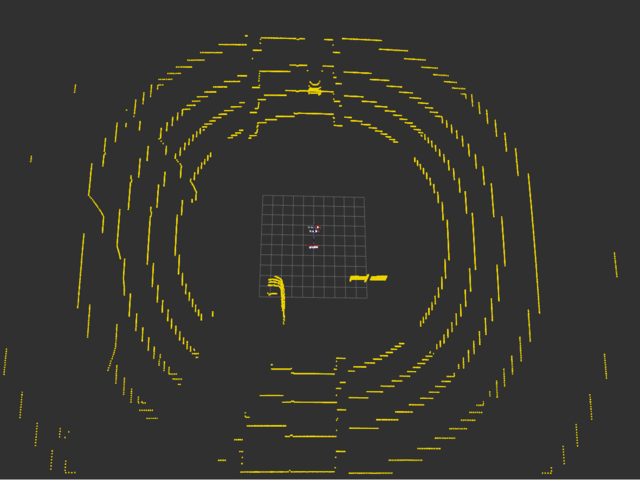
\includegraphics[width=\textwidth]{Figures/Figures_Cap05/pc_objects.png}
         \caption{Antes de aplicar \textit{k-means}.}
         \label{fig:pc_objects}
    \end{subfigure}
    \hfill
    \begin{subfigure}[b]{0.45\textwidth}
         \centering
         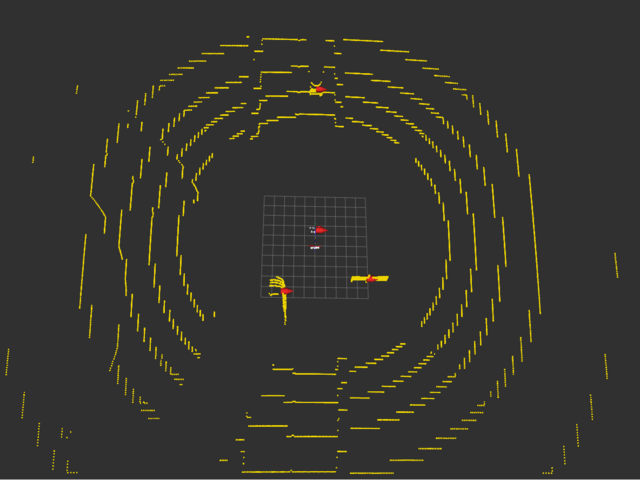
\includegraphics[width=\textwidth]{Figures/Figures_Cap05/pc_centroids.png}
         \caption{Después de aplicar \textit{k-means}.}
         \label{fig:pc_centroids}
     \end{subfigure}
     
    \caption{Nube de puntos antes y después de agrupar mediante \textit{k-means}.}
    \label{fig:pc_clustering}
\end{figure}
%La implementación final de \textit{k-means} en código es en lenguaje C++ debido a los inconvenientes observados con la implementación del mismo algoritmo en Python. En especial se buscó lidiar con el problema de variación de posición para los clusters, para justificar y comprobar este echo se muestra la imagen , donde a y b son el resultado de \textit{k-means} implementado en Python. Es muy notorio que los centroides no son consistentes, si bien detecta los objetos presentes no es posible etiquetar cada centroide con el objeto correspondiente porque cambia constantemente. Por otro lado, con la implementación del mismo algoritmo en C++ se pueden comparar a y b para concluir que los centroides calculados son con
La tarea de detección de objetos concluye al obtener la posición de cada centroide que representa un objeto, este resultado es fundamental para iniciar el proceso de seguimiento de obstáculos.

\section{Empatado} \label{sec:empatado}

Retomando los centroides calculados en \ref{sub:ejemplo_de_implementación_del_algoritmo_K-medias} con el algoritmo de agrupación \textit{k-means} que representan los objetos detectados como la posición media de los puntos de un \textit{cluster} se entiende que conforme el vehículo avanza la nube de puntos cambia en tamaño y forma, como consecuencia el número de centroides varía en cada instante. Este comportamiento presenta la necesidad de saber con certeza que centroide es en cada momento, es decir, se requiere definir si un objeto ha sido previamente detectado con \textit{k-means} y solo ha variado mínimamente su posición. En cambio, si un nuevo objeto es detectado debe ser considerado en la toma de decisiones para evitar colisiones. Dicho de otra forma, el problema por resolver es identificar todos y cada uno de los potenciales obstáculos pues es diferente detectar que identificar objetos. Una vez conocida la posición de los objetos es necesario saber si en cada desplazamiento del vehículo un centroide es el mismo que el anterior o se trata de uno nuevo.

Para empatar dos conjuntos con tamaño $n$ de centroides actual y previo $C_a$ y $C_p$ respectivamente se propone, calcular la distancia euclidiana $d(C_a, C_p)$ entre cada par. 

\begin{equation}
    d(c_{a}, c_{p}) = \sqrt{(c_{a_{x}} - c_{p_{x}})^2 + (c_{a_{y}} - c_{p_{y}})^2 + (c_{a_{z}} - c_{p_{z}})^2}
\end{equation}

Al analizar el resultado de esta operación se obtienen dos posibles escenarios:
\begin{equation}
    d(c_{a}, c_{p}) = \left\lbrace
    \begin{array}{ll}
        \textup{Son el mismo si,} \qquad d(c_{a}, c_{p}) \leq u \\ \\
        \textup{Son diferentes si,} \qquad d(c_{a}, c_{p}) \geq u
    \end{array}
    \right.
\end{equation}
Para el primer caso cuando la distancia $d(c_{a}, c_{p})$ es menor que un umbral $u$ significa que ambos centroides $c_{p}$ y $c_{a}$ representan al mismo objeto, por otro lado cuando la distancia $d(c_{a}, c_{p})$ es mayor que el mismo umbral $u$, implica que $c_{a}$ y $c_{p}$ son dos objetos diferentes. El umbral $u$ es considerado como un valor promedio de las dimensiones de un vehículo pequeño. El algoritmo \ref{alg:matching} describe el empatado de centroides.
\begin{algorithm}
    \begin{algorithmic}[0]
        \REQUIRE Conjunto de centroides previos $C_p$. \\ \parindent=13.5mm Cojunto de centroides actuales $C_a$.
        \ENSURE Conjunto de centroides empatados.
        
        \FORALL{$c_a$} 
            \STATE Obtener el centroide $c$ más cercano a $c_{p}$
            \IF{$d(c, c_a) \geq u$}
                \STATE $c_a$ es un nuevo centroide
                \STATE Agregar $c_a$ al conjunto de centroides empatados.
                %\STATE Crear un nuevo filtro de Kalman con el \textit{id} anterior
            \ELSE
                \STATE $c$ y $c_a$ son el mismo centroide.
            \ENDIF
        \ENDFOR
        \RETURN Conjunto de centroides empatados.
    \end{algorithmic} 
  
    \caption{Algoritmo de Empatado}
    \label{alg:matching}
\end{algorithm}


\section{El filtro de Kalman} \label{sec:el_filtro_de_Kalman}

El filtro de Kalman fue desarrollado por Rudolf E. Kalman en 1960, en principio fue conocido como una solución recursiva al problema de filtrado lineal con datos discretos. En la actualidad es uno de los algoritmos de estimación más importantes y comunes porque produce estimaciones de variables ocultas basadas en mediciones inciertas e inexactas. 
%También, el filtro de Kalman proporciona una predicción del estado futuro del sistema tomando estimaciones pasadas. 

En general, el filtro de Kalman proporciona un método recursivo para estimar el estado futuro de un sistema dinámico en presencia de ruido. El objetivo del filtro es obtener la mejor estimación de un estado \textit{``x''} en el \textit{``k-ésimo''} paso de tiempo dada una estimación previa en combinación con entradas conocidas. Este filtro sirve para estimar estados futuros del sistema cuando se tiene ruido que se adiciona al modelo (ruido de proceso) y a las señales medidas (ruido de medición), además, considera que existe un modelo que relaciona los estados del sistema con las mediciones realizadas (provenientes de los sensores). El proceso de estimación tiene dos dificultades que deben ser superadas. Primero, existe la presencia de vectores de ruido desconocidos e inmedibles. Por lo tanto, una de las tareas es filtrar las perturbaciones no deseadas. La segunda dificultad es que el estado en general no se puede observar directamente desde las salidas previas. Esto significa que la estimación del estado debe reconstruirse en base a la historia temporal de señales y parámetros conocidos \cite{choset2005principles}.

El proceso de estimación mediante el filtro de Kalman es un proceso iterativo y que consta de dos etapas: predicción y actualización: 
\begin{enumerate}
    \item \textbf{Predicción:} En esta etapa el filtro predice el estado, incertidumbre y error siguiente de acuerdo a un modelo del sistema, sin tomar en cuenta el ruido de proceso.
    \item \textbf{Actualización:} Este paso utiliza la información del sensor o sensores utilizados para corregir las estimaciones mediante la diferencia entre valores medidos y valores predichos, posteriormente se calcula una ganancia de Kalman que actualizará los nuevos valores de estado, incertidumbre y error.
    La salida del paso de actualización sirve de retroalimentación al paso de predicción, este proceso continúa hasta que la diferencia entre valor predicho y valor medido tiende a cero.
\end{enumerate}

La figura \ref{fig:kalman_filter_chart} ilustra estos dos pasos.
\begin{figure}[h]
    \centering
    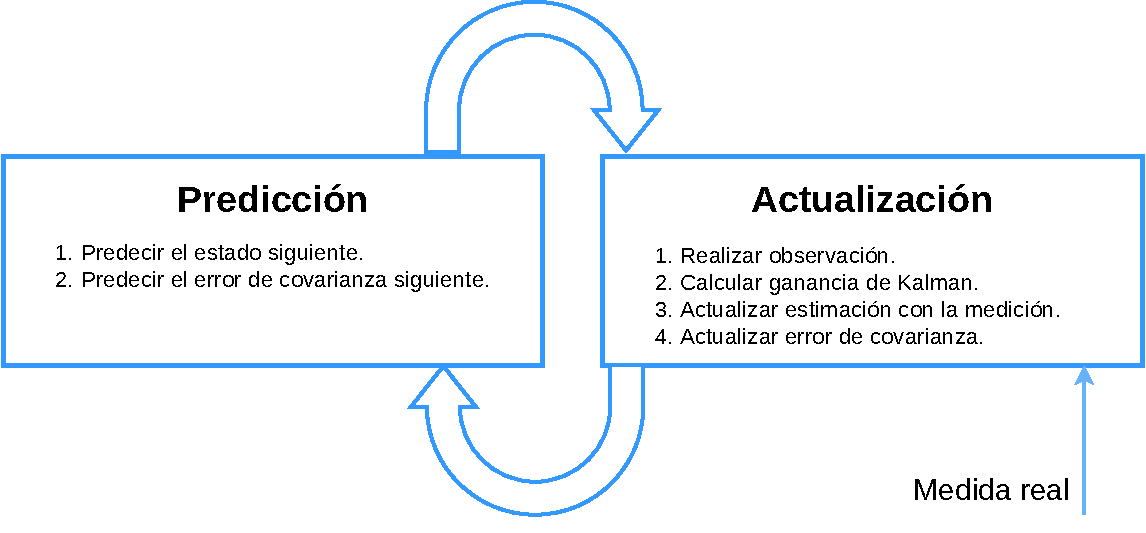
\includegraphics[width=0.75\textwidth]{Figures/Figures_Cap05/kalman_filter_chart.pdf}
    \caption{Etapas del filtro de Kalman.}
    \label{fig:kalman_filter_chart}
\end{figure}

\subsection{El filtro de Kalman extendido} \label{sub:el_filtro_de_Kalman_extendido}

En esencia el filtro de Kalman fue diseñado para estimación de sistemas lineales. Sin embargo, en aplicaciones reales, la mayoría de los sistemas son no lineales, por esta razón, el filtro de Kalman extendido representa una mejora del filtro de Kalman original. El EKF (Extended Kalman Filter) por sus siglas en inglés tiene la facilidad de predecir el estado futuro de un sistema no lineal aplicando métodos de linealización como la matriz jacobiana.

El algoritmo para el filtro de Kalman extendido es descrito con los mismos pasos de predicción y actualización como en el caso de sistemas lineales. Con la diferencia de que en cada estimación de estado, se realiza una linealización del sistema.

\subsection{Estimación de posición y velocidad con el filtro de Kalman extendido} \label{sub:estimación_de_posición_y_velocidad_con_el_filtro_de_kalman_extendido}

El EKF es utilizado en aplicaciones de seguimiento, navegación, control de vehículos y guía. En el caso de un vehículo autónomo se puede usar el filtro para predecir el siguiente movimiento que realizarán los vehículos detectados al frente o los costados de él. El proceso se logra en función de los datos que recibe el vehículo autónomo, específicamente el conjunto de centroides previamente calculados y posteriormente empatados.

Para este trabajo se busca un modelo que permita predecir posición \textit{p} y velocidad \textit{v} de los objetos detectados. En pocas palabras, se busca hacer un seguimiento de objetos (vehículos).
\begin{figure}[h]
    \centering
    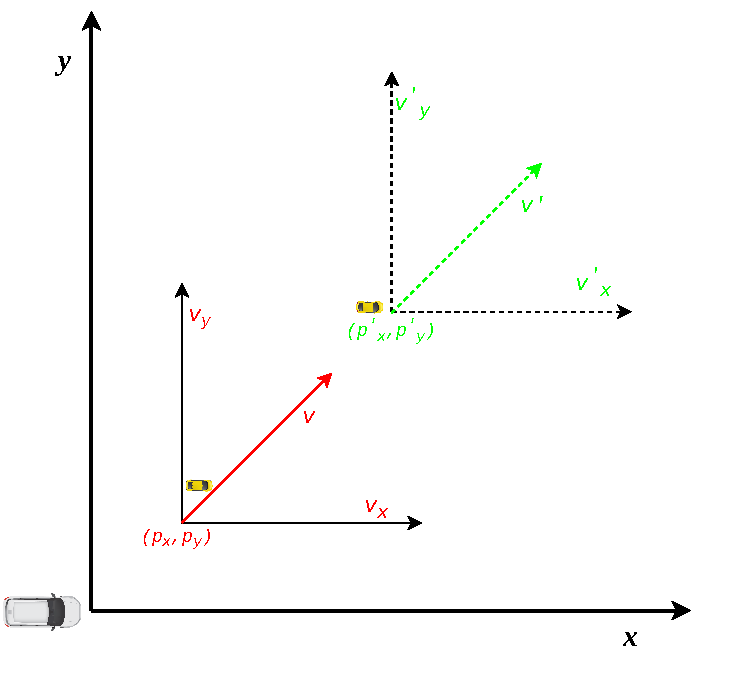
\includegraphics[width=0.75\textwidth]{Figures/Figures_Cap05/ekf_pose_velocity.pdf}
    \caption{Posición y velocidad de un vehículo detectado.}
    \label{fig:ekf_pose_velocity}
\end{figure}

Considerar un entorno 2D como en la imagen \ref{fig:ekf_pose_velocity}, el vehículo autónomo (en color gris) se encuentra en el origen del sistema de referencia $(x, y)$, uno de los posibles vehículos (en color amarillo) detectados previamente, tiene posición $(p_x, p_y)$ y velocidad $(v_x, v_y)$. Dado que se conoce la posición del vehículo detectado se puede obtener la velocidad del mismo como la derivada de la posición $p$ respecto al tiempo $t$. 
\begin{equation*}
    v = \frac{dp}{dt}
\end{equation*}

Mientras que la aceleración es la derivada de la velocidad, en este trabajo se considera velocidad $v$ constante del vehículo detectado en todo momento, por lo tanto, se tiene aceleración $a = 0$

\begin{equation*}
    a = \frac{dv}{dt} = 0
\end{equation*}

De esta manera el sistema por estimar es el siguiente:
\begin{equation*}
    \left\lbrace
    \begin{array}{ll}
        \frac{dp}{dt} = v \\
        \\
        \frac{dv}{dt} = 0
    \end{array}
    \right.
\end{equation*}

y para el caso discreto del modelo anterior se tiene:
\begin{equation*}
    \left\lbrace
    \begin{array}{ll}
        p_{k+1} = p_{k} + \Delta t \hspace{0.1cm} v_{k} + w \\
        \\
        v_{k+1} = v_{k} + w
    \end{array}
    \right.
\end{equation*}

Este sistema permite estimar posición y velocidad de un vehículo detectado. A continuación, se representa este modelo aplicado a la componente $x$ del sistema de referencia de la imagen \ref{fig:ekf_pose_velocity} para fines prácticos. En el caso de la componente $y$ es de la misma forma. Entonces, el sistema de posición y velocidad para la componente $x$ se expresa como:
\begin{equation}
    x=\begin{pmatrix} 
        p_x \\
        v_x
    \end{pmatrix}
    =
    \begin{pmatrix}
        p_{x} + \Delta t \hspace{0.1cm} v_{x} + w \\
        v_{x} + w
    \end{pmatrix}
    \label{eqn:system_pose_vel}
\end{equation}

Y el estado estimado siguiente es:
\begin{equation}
    x'=\begin{pmatrix} 
        p'_x \\
        v'_x
    \end{pmatrix}
    =
    \begin{pmatrix}
        p'_{x} + \Delta t \hspace{0.1cm} v'_{x} + w \\
        v'_{x} + w
    \end{pmatrix}
\end{equation}

donde \textit{x} es el vector de estados, $\Delta t$ es el paso de muestreo, $p_{x}$ y $v_{x}$ son velocidad y posición actual respectivamente y $w$ es ruido de proceso con matriz de covarianza $Q$. El modelo de observación para el filtro es:
\begin{equation}
    z_k = x_k + w
\end{equation}

con $v = 0$, $w$ es ruido de medición con matriz de covarianza $R$. Las mediciones para $z_k$ son las posiciones del conjunto de centroides calculados y empatados. Ahora, la estimación de posición y velocidad consta de los siguientes pasos:

\textbf{Predicción:} Con base en el modelo de posición y velocidad se predice el estado siguiente considerando ruido gaussiano para el modelo de estado y el modelo de medición, como sigue:
\begin{align*} 
    \hat{x}_{k|k-1} &= f(\hat{x}_{k-1|k-1}, u_{k}) \\
    \hat{P}_{k|k-1} &= F_k P_{k-1|k-1} F_{k}^{T} + Q_{k} \\
    \hat{z}_{k|k-1} &= \hat{x}_{k|k-1}
\end{align*}
    
donde $P$ es la matriz de covarianza para el error de estimación, $F_k$ es el Jacobiano (\ref{eqn:f_jacobian}) de la función $f$ (\ref{eqn:system_pose_vel}) y $\hat{z}$ es modelo de observación.
\begin{equation}
    F_k = \begin{pmatrix}
        1 & \Delta t \\
        0 & 1
    \end{pmatrix}
    \label{eqn:f_jacobian}
\end{equation}

Para comenzar la estimación es necesario asignar un valor inicial a la matriz $P$ de ruido de proceso. En este ejemplo $P$ se inicializa con la matriz identidad.

\textbf{Actualización:} La corrección de la estimación se calcula de acuerdo a los errores de observación y estimación. Para el paso de actualización se utilizan las siguientes ecuaciones:
\begin{align*}
    y_k &= z_{k} - h(\hat{x}_{k|k-1}) \\
    S_k &= H_k P_{k|k-1} H_{k}^{T} + R_k \\
    K_k &= P_{k|k-1} H_{k}^T S_{k}^{-1} \\
    \hat{X}_{k|k} &= \hat{x}_{k|k-1} + K_k y_{k} \\
    P_{k|k} &= (I - K_k H_k) P_{k|k-1}
\end{align*}

donde $y_k$ es un residual de medición, $H$ es el Jacobiano (\ref{eqn:h_jacobian}) del modelo de observación respecto a los estados, la matriz $K_k$ es llamada ganancia de Kalman. Las matrices $Q_k$ y $R_k$ para ruido de proceso y ruido de medición respectivamente, son:
\begin{equation*}
    Q_k = \begin{pmatrix}
        0.01 & 0 \\
        0 & 0.01
    \end{pmatrix}
\end{equation*}
y $R_k = 0.1$ es un escalar. El paso de muestreo $\Delta t$ es $0.05 [s]$.
\begin{equation}
    H_k=\begin{pmatrix}
            1 & 0
        \end{pmatrix}
    \label{eqn:h_jacobian}
\end{equation}

Las ecuaciones correspondientes a los pasos de predicción y actualización en forma numérica para la primera iteración son de la forma:

\textbf{Predicción}
\begin{align*}
    \hat{x}&=\begin{pmatrix}1 & \Delta t \\ 0 & 1 \end{pmatrix} \begin{pmatrix} p_x \\ v_x \end{pmatrix} = \begin{pmatrix} p'_{x} \\ v'_{x} \end{pmatrix} \\ \\
    \hat{P}&=\begin{pmatrix} 1 & \Delta t \\ 0 & 1 \end{pmatrix} \begin{pmatrix} 1 & 0 \\ 0 & 1 \end{pmatrix} \begin{pmatrix} 1 & 0 \\ \Delta t & 1 \end{pmatrix} + \begin{pmatrix} 0.01 & 0 \\ 0 & 0.01 \end{pmatrix}
\end{align*}

\textbf{Actualización}
\begin{align*}
    y&=\begin{pmatrix} p_{ox} \\ v_{ox} \end{pmatrix} - \begin{pmatrix} 1 & 0 \end{pmatrix} \begin{pmatrix} p'_{x} \\ v'_{x} \end{pmatrix} \\ \\
    S&=\begin{pmatrix} 1 & 0 \end{pmatrix} \begin{pmatrix} 1 & 0 \\ 0 & 1 \end{pmatrix} \begin{pmatrix} 1 \\ 0 \end{pmatrix} + 0.1 \\ \\
    K&=\begin{pmatrix} 1 & 0 \\ 0 & 1 \end{pmatrix} \begin{pmatrix} 1 \\ 0 \end{pmatrix} \frac{1}{S} \\ \\
    x&=\begin{pmatrix} p'_{x} \\ v'_{x} \end{pmatrix} + K y \\ \\
    P&=\left( \begin{pmatrix} 1 & 0 \\ 0 & 1 \end{pmatrix} - k \begin{pmatrix} 1 & 0    \end{pmatrix} \right) \begin{pmatrix} 1 & 0 \\ 0 & 1 \end{pmatrix}
\end{align*}

Para efectos de implementación en código del Filtro de Kalman Extendido, se optó por crear una clase que contuviera las etapas de predicción y actualización. Después de realizar el proceso de empatado, cada centroide tendrá su propio filtro de Kalman. Mientras $c_a$ y $c_p$ sean el mismo objeto su respectivo filtro de Kalman actualizará posición y velocidad. En el caso de que $c_a$ y $c_p$ sean objetos distintos se creará un nuevo filtro de Kalman para $c_a$.
\newpage

\begin{lstlisting}[language=Python]
# CREATE N OBJECTS
filters = [ [ c, Kalman_Filter() ] for c in centroids ] 

for nc in centroids:
    # COMPUTE DISTANCES
    distances = [ 
        math.sqrt(
            (nc[0] - lc[0])** 2 + 
            (nc[1] - lc[1])** 2 + 
            (nc[2] - lc[2])** 2 
        ) for lc in last_centroids
    ] 
    # GET CLOSER CENTROID (c)
    min_distance = min(distances)
    closer_centroid = last_centroids[
        distances.index(min_distance)
    ]
    closer_idx = distances.index(min_distance)
    if min_distance > threshold: 
        # NC IS A NEW CENTROID, CREATE A NEW OBJECT
        filters[closer_idx] = [ nc, Kalman_Filter() ] 
    else:
        # NC AND C ARE THE SAME, UPDATE MEASURE
        filters[closer_idx][0] = nc 

# APPLY EKF TO FILTERS MATCHED
for c,kalman_filter in filters:
    kalman_filter.ekf(c)
\end{lstlisting}
\hfill

La porción de código anterior representa las tareas de empatado de centroides y estimación de posición y velocidad con el EKF. Al inicio (línea 2) se crean $n$ filtros de Kalman para los objetos detectados. Posteriormente, a partir de la línea 4 y hasta la línea 24 se implementa el algoritmo \ref{alg:matching} para el empatado de centroides actuales y previos. Finalmente, las líneas 27 y 28 efectúan el proceso de filtrado de posición y velocidad con Kalman. Donde la línea 18 hace uso de la clase 'Kalman\_Filter' que calcula cada una de las ecuaciones para predicción y actualización.

Anteriormente, en la sección \ref{sec:simuladores} y en específico con la figura \ref{fig:pc_clustering} se mostró el resultado de la detección de objetos mediante el algoritmo de clusterización \textit{k-means}. La imagen \ref{fig:object_detect_tracking} es una visualización con RViz que muestra la conclusión de empatar centroides y realizar una estimación de posición y velocidad con el filtro de Kalman extendido, a cada objeto se le asigna una etiqueta con sus correspondientes valores de posición y velocidad $[x, z]$ filtrados. En \ref{fig:object_tracking_static} se ilustra el seguimiento de objetos estáticos, se estima la posición $p[x, z]$ de un objeto mientras que la velocidad $v[x, z] = [0, 0]$. El caso de seguimiento de objetos en movimiento se muestra en \ref{fig:object_tracking_dynamic} donde; la velocidad $v[x, z] \neq [0, 0]$. Es importante mencionar que las velocidades del vehículo solo aparecen en la componente $z$ porque los vehículos en seguimiento se desplazan solo en dirección vertical.

\begin{figure}[h]
    \centering
    \begin{subfigure}[b]{0.4\textwidth}
         \centering
         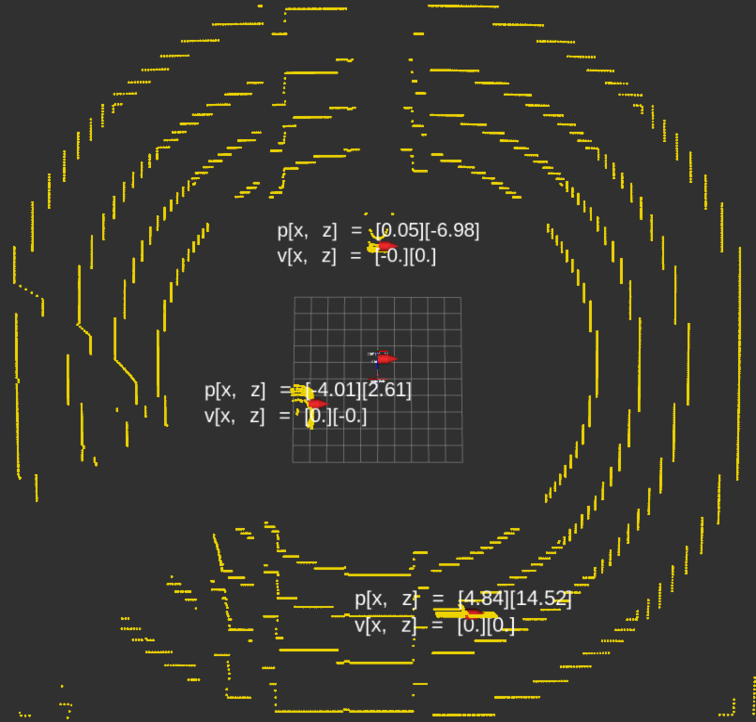
\includegraphics[width=\textwidth]{Figures/Figures_Cap05/object_tracking_static.png}
         \caption{Seguimiento de objetos estáticos.}
         \label{fig:object_tracking_static}
    \end{subfigure}
    \hfill
    \begin{subfigure}[b]{0.4\textwidth}
         \centering
         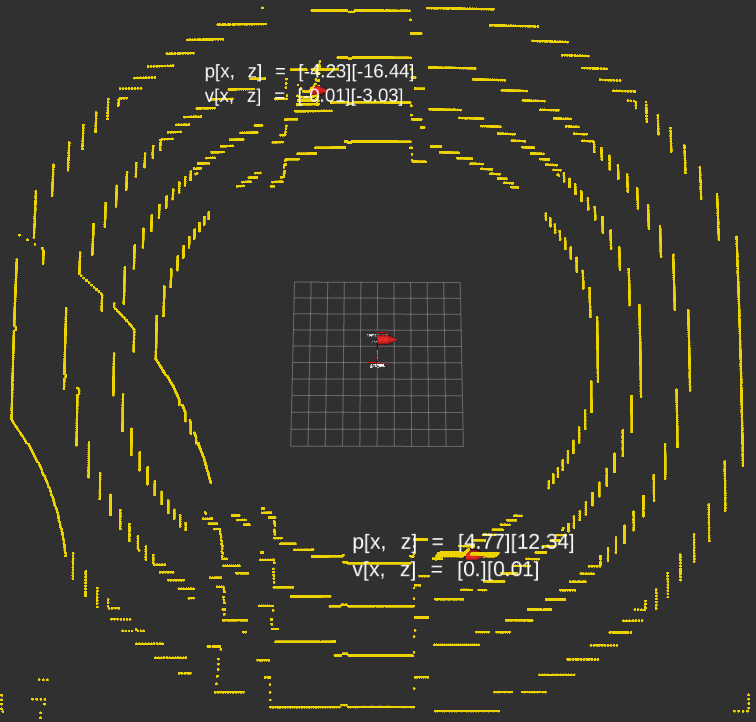
\includegraphics[width=\textwidth]{Figures/Figures_Cap05/object_tracking_dynamic.png}
         \caption{Seguimiento de objetos dinámicos.}
         \label{fig:object_tracking_dynamic}
     \end{subfigure}
     
    \caption{Seguimiento de objetos estáticos y dinámicos.}
    \label{fig:object_detect_tracking}
\end{figure}
\newpage

% CONCLUSIONES DEL CAPÍTULO
Al finalizar este capítulo el vehículo de pruebas cuenta con un sistema de navegación más completo, al incluir detección de objetos con ayuda de \textit{k-means} y seguimiento de objetos con el filtro de Kalman extendido se puede añadir más complejidad al escenario de pruebas descrito en \ref{sec:el_ambiente_de_simulación} y utilizado en el capítulo anterior. En primer lugar, con la aparición de nuevos vehículos en distintas posiciones y en algunos casos con velocidades controladas. Anteriormente, el vehículo autónomo solo podía navegar en un ambiente sin obstáculos utilizando las líneas del carril como guía. En este punto el vehículo aún no es capaz de navegar de manera segura en un ambiente que presente obstáculos, pero con la inclusión de detección y seguimiento de vehículos el vehículo autónomo cuenta con una mejor percepción del ambiente.

En el capítulo siguiente serán esenciales las implementaciones recién añadidas más las del capítulo \ref{cap:seguimiento_de_carriles}, esto con el objetivo de diseñar e implementar diferentes comportamientos y estrategias que le permitan al vehículo autónomo navegar por el circuito que ahora cuenta con obstáculos. Además, se buscarán definir reglas para la toma decisiones en situaciones cercanas a la realidad.


\chapter{Comportamientos} \label{cap:comportamientos}
% BREVE DESCRIPCIÓN DEL CONTENIDO DE ESTE CAPÍTULO
En este capítulo se definirán y diseñarán los comportamientos que necesita el vehículo no tripulado para realizar una conducción autónoma. Al comenzar, en la sección \ref{sec:introducción_a_comportamientos} se da una introducción para los comportamientos esperados del vehículo, enseguida la sección \ref{sec:paradigmas_de_la_robótica} expone los diferentes paradigmas de la robótica y específica que paradigma implementará el robot (vehículo). A continuación, en la sección \ref{sec:comportamientos_del_vehículo} se definen tres comportamientos que el vehículo debe realizar, las subsecciones \ref{sub:crucero}, \ref{sub:mantener_distancia} y \ref{sub:rebase} de esta sección responden a las preguntas de ¿Qué?, ¿Cómo? y ¿Cuándo? se realiza cada comportamiento. Finalmente, la subsección \ref{sub:árbitro} explica el sistema de decisión que controla los comportamientos.

Para este capítulo las implementaciones en código de los comportamientos así como algún cambio en las leyes de control previamente establecidas son con el lenguaje de programación Python.

\section{Introducción a comportamientos} \label{sec:introducción_a_comportamientos}

Tal como se explicó en la sección \ref{sub:niveles_de_autonomía} de capítulo \ref{cap:antecedentes}, un conductor requiere de diferentes habilidades para realizar funciones tácticas y operativas durante el acto de conducir. También, se mencionó que un vehículo autónomo no cuenta de manera natural con estas habilidades, pero si tiene distintos sensores y algoritmos que le ayudan a percibir y conocer el ambiente donde se encuentra. La respuesta o conjunto de respuestas que puede presentar un vehículo no tripulado en situaciones de viales se conoce como comportamiento, la forma en que el robot (vehículo) utiliza las herramientas con las que cuenta son clave para definir uno o varios comportamientos. Al igual que un conductor humano, el vehículo autónomo debe responder correctamente ante diferentes situaciones vehiculares, por ejemplo; mantener una ruta, realizar un rebase, frenar repentinamente o incluso controlar cuidadosamente la velocidad y distancia en situaciones de tráfico.

En este trabajo se pretenden desarrollar tres comportamientos que ayuden al vehículo de pruebas a completar la DDT (\textit{Dynamic Driving Task}) para navegación autónoma con situaciones y condiciones cercanas a la realidad, estos comportamientos son:
\begin{enumerate}
    \item \textbf{Crucero:} Para navegación autónoma sin obstáculos.
    \item \textbf{Rebase:} Para navegación autónoma con obstáculos.
    \item \textbf{Mantener Distancia:} Para navegación en situación de tráfico.
\end{enumerate}
Retomando los conceptos de funciones tácticas y operativas descritas en el capítulo \ref{cap:antecedentes}, el vehículo puede y debe cambiar de comportamiento según las condiciones actuales, para ello es necesario contar con un sistema de decisión que haga el cambio entre comportamientos. En secciones posteriores se describirán estos tres comportamientos además de un árbitro encargado para la toma de decisiones.

\section{Paradigmas de la robótica} \label{sec:paradigmas_de_la_robótica}

Una filosofía o conjunto de suposiciones y técnicas que caracterizan un enfoque para una clase de problemas en particular se conoce como paradigma. Un paradigma es además, una forma de ver el mundo como un conjunto implícito de herramientas en la resolución de problemas. Con este concepto, algunos problemas parecen más adecuados para diferentes enfoques. Por lo tanto, ningún paradigma es del todo correcto y mucho menos absoluto, simplemente tienen procesos diferentes \cite{murphy2019introduction}.

%Por ejemplo, existen problemas matemáticos que podrían resolverse en un sistema cartesiano con coordenadas $(x, y, z)$, pero en ocasiones resulta más sencillo resolver el mismo problema mediante el uso de coordenadas polares $(r, \theta)$. En el campo del cálculo, las coordenadas cartesianas y polares representan dos paradigmas diferentes para manipular un problema. Ambos producen respuestas similares y correctas. Sin embargo, alguno de estos paradigmas puede requerir un menor esfuerzo respecto al otro para el mismo problema.

Un ejemplo de esto son los paradigmas de la programación. Cualquier solución a un problema que pueda ser expresada en forma de algoritmo pude ser implementada mediante algún lenguaje de programación y posteriormente ser procesada por una computadora. En programación existen diferentes paradigmas de programación como: imperativo, declarativo, orientado a objetos, reactivo, entre otros. Cada uno de estos paradigmas posee características propias y están diseñados para implementar soluciones a cuestiones particulares. Problemas lógico-matemáticos sencillos pueden ser resueltos mediante cualquiera de estos paradigmas, pues todos permiten alcanzar una solución correcta y la diferencia radica en la cantidad de esfuerzo que requiere cada paradigma.

El ecosistema de la robótica recupera esta misma idea de paradigma. Aplicar el paradigma correcto permite facilitar la resolución de problemas. Por lo tanto, conocer los paradigmas de la robótica e inteligencia artificial es clave para programar con éxito un robot y lograr una meta particular. En la actualidad existen tres paradigmas en robótica: Jerárquico, Reactivo e Híbrido (Deliberativo - Reactivo). Los paradigmas de la robótica se describen de dos maneras diferentes.

\begin{enumerate}
    \item Por la relación que existe entre las tres primitivas de la robótica: Sentir, Planear y Actuar. Por ejemplo, si una función del robot percibe información de los sensores que lo instrumentan y produce una salida útil para otras funciones, entonces esa función entra en la clasificación de Sentido. Si la función está recibiendo información y produce una o más tareas por realizar (avanzar 2 metros, girar a la izquierda y detenerse) se trata de una función en la categoría de Plan. Finalmente, las funciones que producen comandos de salida hacia los actuadores del robot caen dentro de la categoría de Actuar (girar $n$ grados en sentido horario, con velocidad angular $\omega$).
    
    \item Por la forma en que la información de los sensores es procesada y distribuida a través del sistema. En algunos paradigmas la información de los sensores está restringida para ser utilizada de forma especial en cada función del robot. Otros paradigmas esperan que toda la información del o los sensores primero sea procesada por un modelo global y después los subconjuntos del modelo se distribuyan a otras funciones conforme sea necesario.
\end{enumerate}

\subsection{Paradigma jerárquico} \label{sub:paradigma_jerárquico}

El paradigma jerárquico es el método históricamente más antiguo para organizar inteligencia robótica tradicional. Prevaleció fuertemente desde el año de 1967, con la aparición del primer robot con IA, Shakey\cite{kuipers2017shakey}, hasta principios de la década de 1990. Este paradigma funciona de manera descendente, es decir, de arriba hacia abajo y con mucha planificación. Se basa en una visión introspectiva de como piensan los humanos.``Veo una silla, decido sentarme en ella y genero una trayectoria hacia ella evitando obstáculos". Un robot que implementa el paradigma jerárquico, percibe el mundo, planifica la siguiente acción y después actúa (Sensa, Planea y Actúa), ver \ref{fig:hierarchical_paradigm}. Dicho de otro modo, este paradigma es secuencial y ordenado. En cada paso el robot planifica explícitamente el movimiento siguiente. Otra característica fundamental del modelo jerárquico es que toda la información percibida por los sensores tiende a reunirse en un modelo global o una sola representación que el sistema planificador (Planear) utiliza para encaminarse a realizar acciones (Actuar) \cite{murphy2019introduction}. 
%El proceso de ejecución de cada paso en el paradigma jerárquico es: Primero, el robot detecta el mundo y construye un mapa global de este. Después, con los ojos cerrados, planifica todas las acciones necesarias para alcanzar la meta. Posteriormente, el robot actúa para llevar a cabo la primer acción. Al final, cuando el robot ha llevado a cabo la secuencia Sentir-Planear-Actuar \ref{fig:hierarchical_paradigm}, comienza nuevamente el ciclo de manera iterativa.
La detección o el efecto de sentir en el paradigma jerárquico es de manera monolítica: todas las observaciones de los sensores se fusionan en una estructura de datos global , a la que puede acceder el planificador. Esta estructura de datos se conoce como modelo de mundo, donde el término mundo hace referencia tanto al mundo exterior como cualquier otro significado que el robot le atribuya. Dentro de este paradigma el modelo de mundo contiene típicamente:
\begin{enumerate}
    \item Una representación \textit{a priori} del entorno en que el robot opera.
    \item Información de detección del ambiente.
    \item Cualquier conocimiento cognitivo adicional que resulte necesario para realizar una tarea.
\end{enumerate}

El paradigma Jerárquico ofrece diferentes ventajas como: orden en la relación Sensar-Planear-Actuar, fomentar la programación monolítica y funcional. Sin embargo, al ser el más antiguo cuenta con varias desventajas entre las que destacan: lenta ejecución en algoritmos de detección y planificación, Requiere la mayor cantidad de información posible del entorno, además de no toma en cuenta la incertidumbre en sensores y actuadores.

\begin{figure}
    \centering
    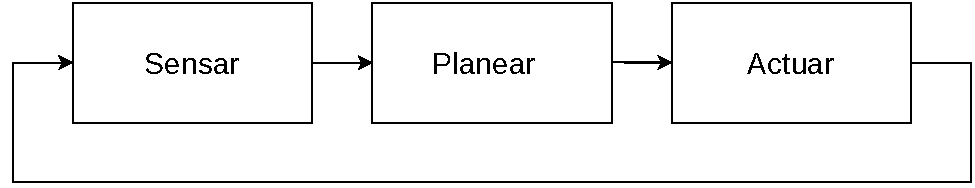
\includegraphics[width=0.8\textwidth]{Figures/Figures_Cap06/hierarchical_paradigm.pdf}
    \caption{Secuencia del Paradigma Jerárquico.}
    \label{fig:hierarchical_paradigm}
\end{figure}

\subsection{Paradigma Reactivo} \label{sub:paradigma_reactivo}

El Paradigma Reactivo surgió a finales de la década de 1980 como solución a problemas que el Paradigma Jerárquico no podía resolver. El modelo reactivo asume que la entrada de una tarea (Actuar) siempre será una salida directa de un sensor (Sensar). Su enfoque fundamental es que todas las acciones del robot son modeladas y realizadas a través de comportamientos. 

Un comportamiento es el conjunto de respuestas que presenta un individuo con relación a su mundo o entorno. Los comportamientos son un mapeo directo de las entradas sensoriales a un patrón de acciones motoras que después se unen para alcanzar una meta. Desde el punto de vista matemático, los comportamientos representan una función de transferencia que transforma entradas sensoriales en comandos de activación \cite{murphy2019introduction}. 

Los sistemas dentro de un paradigma reactivo se componen de comportamientos que mantienen unidos estrechamente la percepción (Sensar) y acción (Actuar), todas las actividades robóticas surgen como resultado de estos comportamientos que operan simultáneamente o en secuencia. La organización de este modelo es Sensar-Actuar sin tomar en cuenta la planificación, la figura  \ref{fig:reactive_paradigm} muestra esto. La percepción en el Paradigma Reactivo es específica o local para comportamiento. Es decir, cada comportamiento tiene acceso directo a uno o más sensores que son independientes de otros comportamientos. En situaciones específicas, más de un comportamiento puede tomar el resultado de un sensor y procesarlo de manera diferente. En esencia, un comportamiento no conoce lo que hace o percibe otro comportamiento. El paradigma reactivo puede combinar comportamientos en una arquitectura mediante dos métodos dominantes: subsunción y suma de campos potenciales.
\begin{figure}
    \centering
    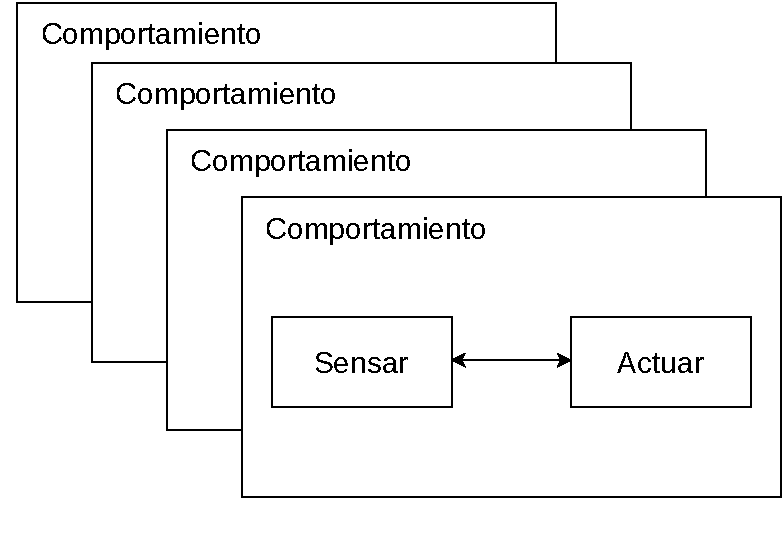
\includegraphics[width=0.5\textwidth]{Figures/Figures_Cap06/reactive_paradigm.pdf}
    \caption{Secuencia del Paradigma Reactivo.}
    \label{fig:reactive_paradigm}
\end{figure}

Las ventajas más reconocidas de este paradigma son los buenos principios de Ingeniería de Software que exhiben los sistemas que lo implementan, los comportamientos se pueden probar de manera independiente. Además, se pueden construir comportamientos más complejos a partir de comportamientos primitivos, existe bajo acoplamiento y alta cohesión. Los comportamientos son inherentemente modulares y fáciles de probar de manera aislada al sistema. Por el contrario, si los comportamientos se implementan de manera deficiente puede derivar en una ejecución lenta. Dentro del paradigma reactivo un robot se vuelve más inteligente mientras más y mejores comportamientos existan. 

Es importante mencionar que el vehículo autónomo de este trabajo toma como base el paradigma reactivo, cada comportamiento que implemente el vehículo debe hacer uso de las herramientas previamente implementadas para efectuar tareas específicas y mientras más comportamientos se definan, el vehículo autónomo tendrá un nivel de independencia más alto.

\subsection{Paradigma Híbrido} \label{sub:paradigma_híbrido}

El paradigma Híbrido o Deliberativo/Reactivo emergió a principios de la década de 1990, es una combinación de muchos de los fundamentos del Paradigma Reactivo y Jerárquico. Bajo las tres primitivas de la robótica, el modelo Deliberativo/Reactivo se puede pensar como Planear y luego Sensar-Actuar (P, S-A), ver figura \ref{fig:hybrid_paradigm}. Donde, la parte de Sensar-Actuar siempre es realizada mediante comportamientos reactivos, mientras que la planificación es resultado de una amplía gama de actividades inteligentes. El término híbrido se da porque la planificación se puede intercalar con la ejecución; luego, en mayor medida, el robot planea un conjunto de comportamientos que más tarde ejecutará por un largo tiempo. La detección también es híbrida; la parte reactiva utiliza representaciones locales en cada comportamiento, mientras que la parte deliberativa usa modelos del mundo global como en el paradigma jerárquico.

Generalmente una arquitectura híbrida tiene los siguientes módulos:
\begin{itemize}
    \item Planificador de misiones
    \item Secuenciador
    \item Administrador de comportamiento
    \item Cartógrafo
    \item Monitor de Rendimiento
\end{itemize}

La regla general para clasificar funciones en deliberativas o reactivas es; funciones que operan con información simbólica forman parte de la capa deliberativa, mientras que las funciones que transforman información de los sensores en comandos de activación van a la capa reactiva. El componente reactivo del modelo está compuesto por comportamientos, por otro lado el deliberativo a menudo se subdivide en capas.
\begin{figure}[h]
    \centering
    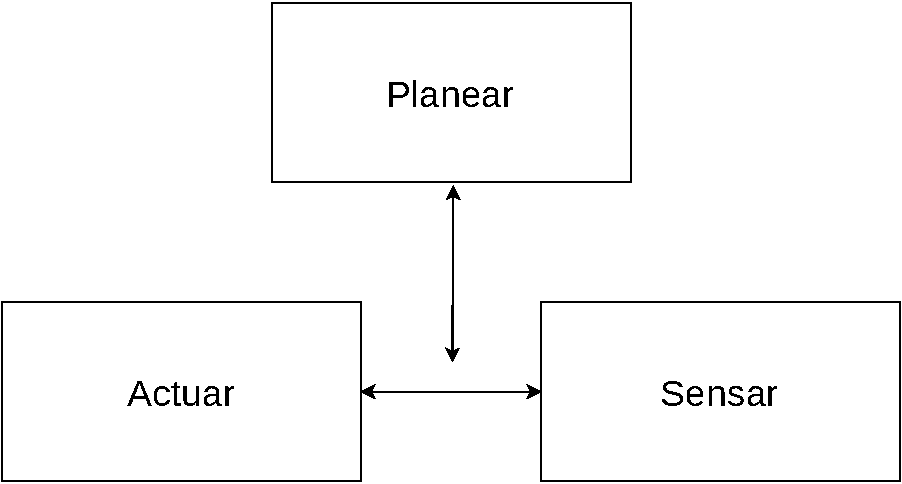
\includegraphics[width=0.5\textwidth]{Figures/Figures_Cap06/hybrid_paradigm.pdf}
    \caption{Secuencia del Paradigma Híbrido.}
    \label{fig:hybrid_paradigm}
\end{figure}

\section{Comportamientos del vehículo} \label{sec:comportamientos_del_vehículo}

\subsection{Crucero} \label{sub:crucero}

De forma similar a como sucede en los sistemas de crucero de un vehículo real, el comportamiento de crucero tiene como objetivo navegar dentro de un circuito vehicular con situaciones controladas y con una velocidad previamente establecida. Estas situaciones incluyen tener un circuito sin obstáculos y mostrar los carriles de la carretera con sus debidas delimitaciones en todo momento, tanto en líneas rectas como en curvas. La figura \ref{fig:cruise_behavior} muestra un escenario con estas condiciones. En otras palabras, el comportamiento de crucero buscar realizar concretamente un seguimiento de carril. Para ello, este comportamiento utiliza el detector y seguidor de carril explicados en el capítulo \ref{cap:seguimiento_de_carriles}, también hace uso de las ecuaciones (\ref{eqn:cruise_speed})-(\ref{eqn:steering_angle}) previamente diseñadas que modelan las leyes de control para las funciones operativas de movimiento lateral y longitudinal respectivamente. Este comportamiento se mantiene activo mientras existan condiciones sin obstáculos en el camino del vehículo.
\begin{figure}[h]
    \centering
    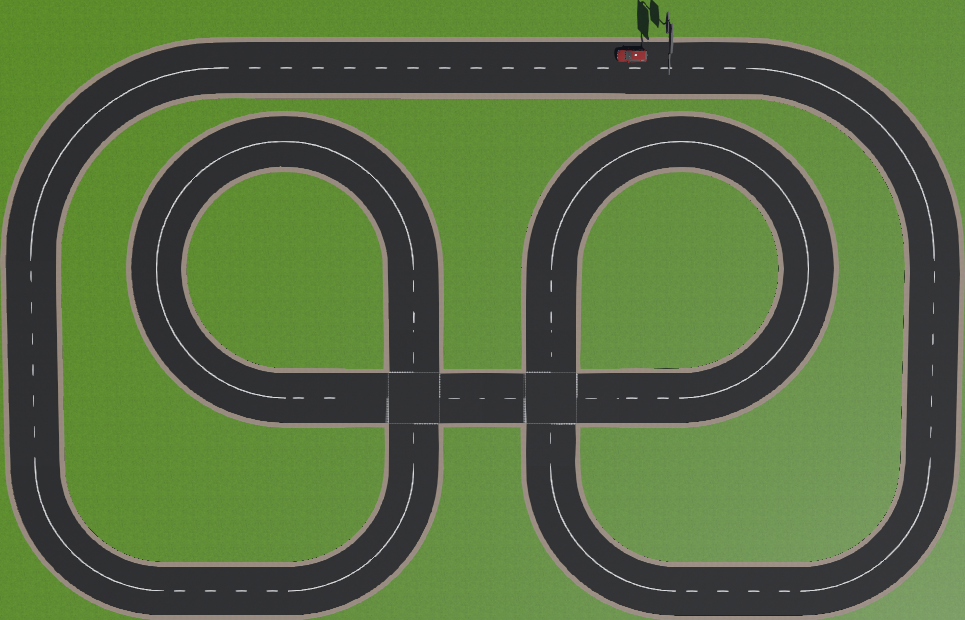
\includegraphics[width=0.5\textwidth]{Figures/Figures_Cap06/crucero.png}
    \caption{Circuito de pruebas sin obstáculos.}
    \label{fig:cruise_behavior}
\end{figure}

\subsection{Mantener distancia} \label{sub:mantener_distancia}

Al incluir vehículos al circuito de pruebas la complejidad en la navegación autónoma aumenta. Este comportamiento como su nombre lo indica pretende mantenerse a distancia con los vehículos presentes en la carretera. El comportamiento de mantener distancia actúa en una situación de tráfico vehicular manteniendo al vehículo autónomo a una distancia segura respecto al vehículo de enfrente para evitar colisiones, ver \ref{fig:keep_distance_behavior}.
%También, se hace uso de la detección y seguimiento de objetos explicados en el capítulo \ref{cap:detección_de_obstáculos}.
Este comportamiento se logra utilizando la detección y seguimiento de carril desarrollados en el capítulo \ref{cap:seguimiento_de_carriles} con una mínima modificación. Primero, la ley de control para el movimiento lateral del vehículo es con la ecuación (\ref{eqn:steering_angle}), que es la misma utilizada para el seguimiento de carril. La diferencia aparece en la ley de control para el movimiento longitudinal, anteriormente se había mencionado que la velocidad del vehículo autónomo sería constante durante todo el recorrido, esto funciona bien para el comportamiento de crucero. Sin embargo, en el caso de seguimiento de vehículos la velocidad debe variar respecto a la distancia del coche de enfrente para no chocar. 
\begin{figure}[h]
    \centering
    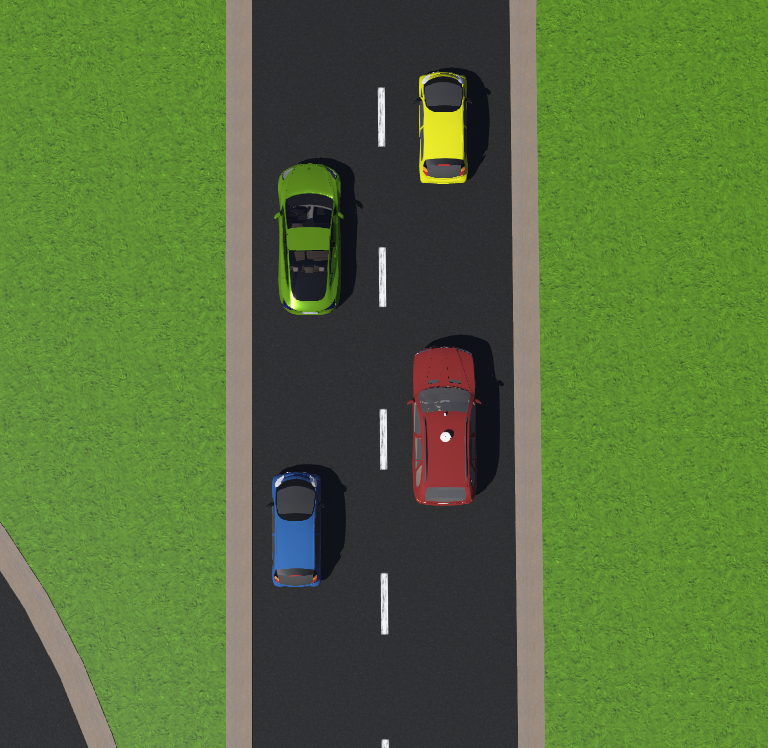
\includegraphics[width=0.5\textwidth]{Figures/Figures_Cap06/keep_distance.png}
    \caption{Ejemplo de posible situación de tráfico.}
    \label{fig:keep_distance_behavior}
\end{figure}

Considerar la figura \ref{fig:safe_distance}, en ella se ilustra una posible situación de tráfico, el vehículo en color rojo es el vehículo autónomo y lo llamaremos $a$, el coche amarillo lo nombraremos $b$. Es evidente que en está situación no se puede manejar libremente solo siguiendo las líneas del carril con velocidad constante. Por ello en este comportamiento cuando el vehículo $b$ se encuentre a una distancia muy cercana con $a$ se debe de disminuir la velocidad de $a$, cuando el vehículo $b$ esté más lejos, la velocidad de $a$ aumenta. Es decir, el coche $a$ aumenta o disminuye su velocidad proporcionalmente a la distancia $d$. Con esta proporción entre velocidad y distancia se logra seguir al vehículo del frente a una distancia segura y evitar colisiones, por otro lado, las colisiones en los laterales se evitan con el seguimiento de carril, pues la ley de control del movimiento lateral mantiene al vehículo autónomo dentro de su carril.
\begin{figure}[h]
    \centering
    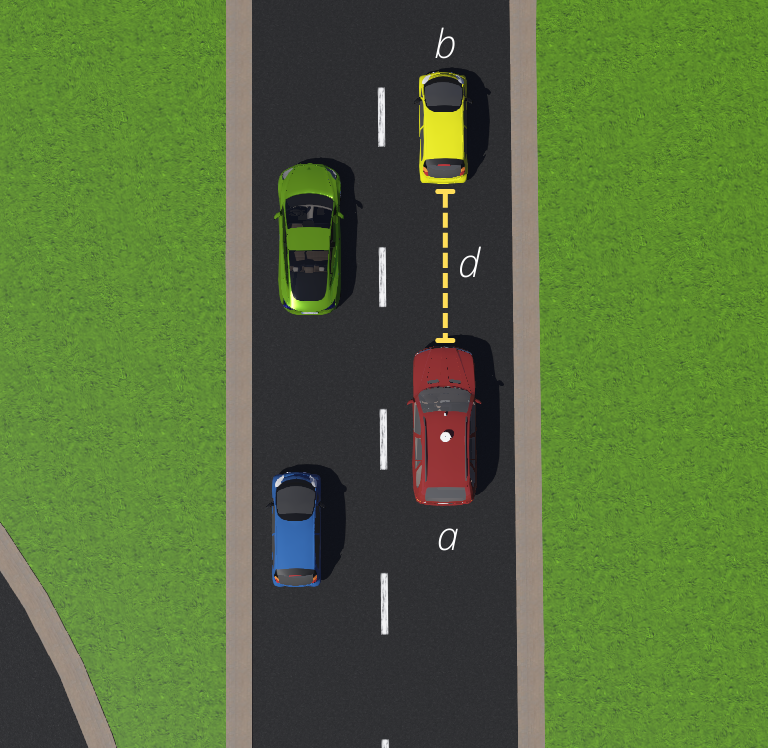
\includegraphics[width=0.5\textwidth]{Figures/Figures_Cap06/safe_distance.png}
    \caption{Distancia Segura, $d(a, b)$.}
    \label{fig:safe_distance}
\end{figure}

La distancia $d$ que existe entre el vehículo autónomo y el vehículo de enfrente la llamaremos ``distancia segura'', ver \ref{fig:safe_distance}. Con esta distancia se calcula la velocidad del vehículo autónomo. Entonces, para este comportamiento la ecuación (\ref{eqn:cruise_speed}) que representa la ley de control de movimiento longitudinal se expresa de la siguiente forma:
\begin{equation}
    v = d * k
    \label{eqn:keep_distance_velocity}
\end{equation}
donde, $d$ es la distancia entre $a$ y $b$, mientras que $k$ es una constante de proporcionalidad para aumentar o disminuir velocidad. El comportamiento mantener distancia entra en acción cuando se presentan situaciones donde no es posible mantenerse en crucero o cuando no se pueda realizar un rebase.

\subsection{Rebase} \label{sub:rebase}

El rebase es un comportamiento especial porque cambia considerablemente las leyes de control previamente establecidas para el movimiento lateral y longitudinal. Un rebase requiere de diferentes acciones que involucran el cambio de dirección en las llantas y mantener la velocidad en un rango aceptable, estas acciones deben de ser bien planeadas para evitar choques con el vehículo por rebasar.

Para implementar un comportamiento de rebase en este trabajo específico se optó por realizarlo en condiciones de lazo abierto, es decir, no existe ningún tipo de retroalimentación como en los comportamientos de crucero y seguimiento de vehículos donde la retroalimentación al sistema provenía del error en los carriles detectados y la distancia segura respectivamente. Se entiende que bajo las normas de conducción vehicular solo se pueden efectuar rebases por el carril izquierdo. Por lo tanto, una vez que se detecta una posible situación de rebase se ejecuta una máquina de estados específica que cumple con esta acción, ver figura \ref{fig:pass}. A continuación se enuncia la secuencia de pasos a seguir para realizar un rebase:
\begin{enumerate}
    \item Girar a la izquierda $t$ segundos.
    \item Girar a la derecha $t/2$ segundos para alinear.
    \item Avanzar en línea recta $t$ segundos.
    \item Girar a la derecha $t$ segundos.
    \item Girar a la izquierda $t/2$ segundos para alinear.
    \item Avanzar en línea recta $t$ segundos.
\end{enumerate}
\begin{figure}[h]
    \centering
    \includegraphics[width=0.5\textwidth]{Figures/Figures_Cap06/rebase.png}
    \caption{Situación de rebase.}
    \label{fig:pass}
\end{figure}


Una vez conocidos estos pasos es fácil diseñar una máquina de estados para rebase, la figura \ref{fig:pass_sm} representa la carta ASM para esta máquina de estados.

Durante el rebase se considera una velocidad constante pero menor a la velocidad utilizada en el seguimiento de carril.
\begin{equation}
    v_r < v
\end{equation}
Para controlar el \textit{steering} del vehículo en giros a la izquierda el ángulo de dirección es $\delta < 0$ y en giros a la derecha $\delta > 0$. Además, se toma en cuenta el ángulo de dirección actual del vehículo, de esto modo la ecuación (\ref{eqn:steering_angle}) para movimiento lateral se transforma en:
\begin{equation}
    \delta = \delta_{actual} + \theta
    \label{eqn:right_steering}
\end{equation}
para giros a la derecha, y
\begin{equation}
    \delta = \delta_{actual} - \theta
    \label{eqn:left_steering}
\end{equation}
para giros a la izquierda.
\begin{figure}[h]
    \centering
    \includegraphics[width=1.0\textwidth]{Figures/Figures_Cap06/sm_pass.pdf}
    \caption{Máquina de estados para acción de rebase.}
    \label{fig:pass_sm}
\end{figure}

En las ecuaciones (\ref{eqn:right_steering})-(\ref{eqn:left_steering}), $\theta$ representa un ángulo constante para provocar un giro a la izquierda o a la derecha según corresponda. Esta constante $\theta$ como el tiempo $t$ fueron obtenidos mediante experimentación del comportamiento de rebase. El resultado esperado al implementar la carta ASM de la figura \ref{fig:pass_sm} es el que se muestra en \ref{fig:pass_behavior}, donde se observa la secuencia de pasos que debe de seguir el vehículo autónomo para lograr un rebase seguro. El comportamiento de rebase se activa siempre y cuando existan condiciones seguras para evitar choques, es decir, que no existan vehículos cercanos al frente, por detrás y al costado izquierdo del vehículo. También, se considera que lo más seguro después de completar un rebase es volver al comportamiento de crucero.

\begin{figure}[h]
    \centering
    \includegraphics[width=0.15\textwidth]{Figures/Figures_Cap06/pass_1.png}
    \includegraphics[width=0.15\textwidth]{Figures/Figures_Cap06/pass_2.png}
    \includegraphics[width=0.15\textwidth]{Figures/Figures_Cap06/pass_3.png}
    \includegraphics[width=0.15\textwidth]{Figures/Figures_Cap06/pass_4.png}
    \includegraphics[width=0.15\textwidth]{Figures/Figures_Cap06/pass_5.png}
    \caption{Secuencia para comportamiento de rebase.}
    \label{fig:pass_behavior}
\end{figure}

\subsection{Árbitro} \label{sub:árbitro}

El árbitro es un sistema que permite tomar decisiones y cambiar al comportamiento más adecuado en cada situación que se presente durante la navegación autónoma en el circuito. Para elegir entre los comportamientos crucero, mantener distancia y rebase, el árbitro percibe el ambiente del vehículo en todo momento. Mientras el vehículo avanza se ejecuta el algoritmo de agrupación \textit{k-means} de la sección \ref{sub:ejemplo_de_implementación_del_algoritmo_K-medias}, posteriormente el EKF diseñado en \ref{sub:estimación_de_posición_y_velocidad_con_el_filtro_de_kalman_extendido} estima la posición y velocidad de los obstáculos (vehículos) detectados. Con base en estas mediciones el árbitro es capaz de definir diferentes escenarios y elegir el comportamiento que mejor se acople.

Dentro del circuito es posible que existan múltiples vehículos en diferentes posiciones, sin embargo, para este proyecto se toman en cuenta cuatro posibles obstáculos que influyan en el cambio de comportamiento del vehículo. Considerar la figura \ref{fig:obstacle_zones}, en ella se muestra el vehículo de pruebas en color rojo y los objetos en color amarillo son las posibles posiciones de los vehículos obstáculo. Las etiquetas de los vehículos amarillos corresponden a la zona donde se encuentran, para estas zonas se considera al vehículo autónomo (rojo) como el punto de origen,  las zonas son:
\begin{enumerate}
    \item Norte (N)
    \item Este  (E)
    \item Noroeste (NE)
    \item Suroeste (SE)
\end{enumerate}

\begin{figure}[h]
    \centering
    \includegraphics[width=0.25\textwidth]{Figures/Figures_Cap06/zones.pdf}
    \caption{Zonas de obstáculos.}
    \label{fig:obstacle_zones}
\end{figure}

Teniendo en cuenta esta configuración de zonas es claro que un vehículo puede o no ocupar una zona, al considerar cuatro posibles vehículos como obstáculos se pueden presentar $4^2 = 16$ estados posibles. Cada uno de estos estados se aprecian abiertamente en la figura \ref{fig:states}, donde 0 representa una zona ocupada y 1 para zona libre.
\newpage
\begin{figure}[h]
    \centering
    \includegraphics[width=0.75\textwidth]{Figures/Figures_Cap06/states.pdf}
    \caption{Estados considerados.}
    \label{fig:states}
\end{figure}

\newpage
La información de los posibles estados de la figura \ref{fig:states} se puede ver en forma tabular. A continuación, el cuadro \ref{tab:states} indica cual es el comportamiento más adecuado para cada estado.
\begin{table}[h]
    \begin{center}
        \begin{tabular}{cccc||l}
        \hline
            E & SE & NE & N & Comportamiento\\ \hline \hline
            0 & 0 & 0 & 0 & Mantener Distancia\\ 
            0 & 0 & 0 & 1 & Crucero\\
            0 & 0 & 1 & 0 & Mantener Distancia\\
            0 & 0 & 1 & 1 & Crucero\\
            0 & 1 & 0 & 0 & Mantener Distancia\\
            0 & 1 & 0 & 1 & Crucero\\
            0 & 1 & 1 & 0 & Mantener Distancia\\
            0 & 1 & 1 & 1 & Crucero\\
            1 & 0 & 0 & 0 & Mantener Distancia\\
            1 & 0 & 0 & 1 & Crucero\\
            1 & 0 & 1 & 0 & Rebase\\
            1 & 0 & 1 & 1 & Crucero\\
            1 & 1 & 0 & 0 & Mantener Distancia\\
            1 & 1 & 0 & 1 & Crucero\\
            1 & 1 & 1 & 0 & Rebase\\
            1 & 1 & 1 & 1 & Crucero\\ \hline
        \end{tabular}
    \end{center}
    \caption{Tabla de estados.}
    \label{tab:states}
\end{table}

Con la tabla anterior se puede notar que en 6 de los 16 estados ($37.5\%$) el comportamiento más adecuado es mantener distancia, en 8 ocasiones ($50.0\%$) lo más apropiado es la conducción mediante el comportamiento de crucero y solo en 2 de los 16 estados ($12.5\%$) existen condiciones seguras para realizar un rebase de vehículo. 

De forma similar a la implementación del comportamiento de rebase, el árbitro también hace uso de una máquina de estados donde se incluyen todas las condiciones vistas en la tabla \ref{tab:states} para escoger el comportamiento apropiado. La carta ASM que representa a la máquina de estados del árbitro se puede ver en \ref{fig:main_sm}.
\begin{figure}[h]
    \centering
    \includegraphics[width=0.7\textwidth]{Figures/Figures_Cap06/main_sm.pdf}
    \caption{Máquina de estados para decidir comportamiento.}
    \label{fig:main_sm}
\end{figure}

Mediante esta máquina de estados el árbitro puede habilitar y deshabilitar comportamientos según sea necesario, además puede enviar y recibir las variables de ``distancia segura'' y ``rebase terminado'' para el control de los comportamientos de mantener distancia y rebase respectivamente. 

Al concluir este capítulo se definieron los comportamientos con los que contará el vehículo autónomo, cada uno de ellos es utilizado en situaciones y tareas específicas. También, se mencionó que un árbitro estará a cargo de la elección. Es posible que el árbitro sea la parte más importante del sistema de navegación del vehículo autónomo porque es el encargado de decidir el comportamiento adecuado a cada situación, de modo que, si llega a fallar en la elección puede tener como consecuencia salir del camino o en un caso más extremo chocar con algún vehículo. Con estas nuevas características, el sistema de navegación del vehículo autónomo es mucho más completo y ahora debe ser capaz de conducir de forma autónoma en espacios supervisados. 

En el capítulo siguiente se expondrán diferentes retos de navegación para el vehículo autónomo donde se pondrán a prueba todos los módulos diseñados e implementados como el detector y seguidor de carril, el sistema para detección y seguimiento de objetos, así como el árbitro que deberá seleccionar el comportamiento apropiado en cada situación como ya se ha mencionado reiteradamente.


\chapter{Pruebas y resultados} \label{cap:pruebas_y_resultados}
% Breve descripción del capítulo
El capítulo de pruebas y resultados como su nombre lo indica pretende observar el desempeño del sistema de navegación en diferentes situaciones para interpretar los resultados obtenidos. Al comienzo de este capítulo, en la sección \ref{sec:integración_mediante_la_plataforma_ROS} se describen de forma breve todos y cada uno de los nodos desarrollados para el sistema de navegación. En las posteriores secciones \ref{sec:pruebas_de_navegación_sin_obstáculos}, \ref{sec:pruebas_de _navegación_con_obstáculos} y \ref{sec:pruebas_de_navegación_con_obstáculos_en_movimiento} se exponen las pruebas para navegación sin obstáculos, navegación con obstáculos y navegación con obstáculos en movimiento respectivamente. En cada una de estas secciones se menciona qué se busca comprobar además de mencionar las condiciones que son requeridas, finalmente se exponen los resultados obtenidos durante cada prueba.

\section{Integración mediante la plataforma ROS} \label{sec:integración_mediante_la_plataforma_ROS}

El sistema navegación del vehículo autónomo es logrado a través de una combinación de diferentes tecnologías. Como se mencionó en capítulos anteriores Webots es el simulador utilizado para modelar los escenarios, vehículos de obstáculo y el propio vehículo autónomo. Los controladores y supervisores que utilizan los elementos modelados en el simulador fueron desarrollados con el lenguaje de programación Python. Por otro lado, los nodos que conforman al sistema de navegación fueron desarrollados en su mayoría con Python y otros más con C++, finalmente, la parte de comunicación por mensajes entre nodos es con la plataforma ROS.

A continuación se describen brevemente cada uno de los nodos que forman parte del sistema de navegación del vehículo.

\hfill

\textbf{\textit{ros\_car\_controller}}
\begin{itemize}
    \item \textbf{Descripción:} Nodo responsable de obtener y comunicar la información de los sensores(Cámara y LIDAR), así como el ángulo de dirección actual del vehículo autónomo. Además, sitúa los valores de velocidad y ángulo de dirección en los actuadores correspondientes del vehículo autónomo.
    \item \textbf{Tópicos publicados:} 
    \begin{itemize}
        \item /current\_steering
        \item /camera/rgb/raw
        \item /point\_cloud
    \end{itemize}
    \item \textbf{Tópicos suscritos:}
    \begin{itemize}
        \item /goal\_speed
        \item /goal\_steering
    \end{itemize}
\end{itemize}
\hfill

\textbf{\textit{lane\_detect}}
\begin{itemize}
    \item \textbf{Descripción:} Este nodo tiene la finalidad de procesar una imagen RGB que proviene de la cámara del vehículo para hacer la detección de carril, hace uso de las herramientas de detector de bordes de Canny y detección de líneas rectas con transformada Hough explicadas en el capítulo \ref{cap:seguimiento_de_carriles}. El resultado de la ejecución de este nodo son dos líneas rectas en forma polar que corresponden a los bordes del carril identificado.
    \item \textbf{Tópicos publicados:}
    \begin{itemize}
        \item /left\_lane
        \item /right\_lane
    \end{itemize}
    \item \textbf{Tópicos suscritos:} 
\begin{itemize}
    \item /camera/rgb/raw
\end{itemize}
\end{itemize}
\hfill

\textbf{\textit{object\_detect}}
\begin{itemize}
    \item \textbf{Descripción:} Nodo responsable de obtener la nube de puntos del sensor LIDAR, filtrarla y agruparla con el algoritmo \textit{k-means}. La salida de este nodo es un conjunto de centroides que representan la posición media de los obstáculos detectados.
    \item \textbf{Tópicos publicados:}
    \begin{itemize}
        \item /object\_pose
    \end{itemize}
    \item \textbf{Tópicos suscritos:}
    \begin{itemize}
        \item /point\_cloud
    \end{itemize}
\end{itemize}

\newpage

\textbf{\textit{object\_tracking}}
\begin{itemize}
    \item \textbf{Descripción:} Este nodo se encarga de empatar y estimar posición y velocidad de los obstáculos detectados con el algoritmo \textit{k-means}. Para el empatado utiliza el algoritmo \ref{alg:matching} y para la estimación el filtro de Kalman diseñado en la sección \ref{sub:estimación_de_posición_y_velocidad_con_el_filtro_de_kalman_extendido} del capítulo \ref{cap:detección_de_obstáculos}. Como resultado de este proceso se obtiene un conjunto de pares [obstáculo, EKF], donde ``obstáculo'' es un identificador para cada obstáculo detectado y ``EKF'' es su correspondiente filtro de Kalman con posición y velocidad estimadas.
    \item \textbf{Tópicos publicados:} 
    \begin{itemize}
        \item /filter\_pose
    \end{itemize}
    \item \textbf{Tópicos suscritos:}
    \begin{itemize}
        \item /object\_pose
    \end{itemize}
\end{itemize}
\hfill

\textbf{\textit{object\_avoidance}}
\begin{itemize}
    \item \textbf{Descripción:} El sistema de árbitro explicado en el capítulo \ref{cap:comportamientos} es representado por este nodo. Define el conjunto de zonas ocupadas utilizando las posiciones estimadas con el EKF, implementa la máquina de estados de la figura \ref{fig:main_sm} y comunica las señales de habilitación para los comportamientos de crucero, mantener distancia y rebase. También, para el comportamiento de mantener distancia, calcula y comunica la distancia que existe entre el vehículo autónomo y el coche de enfrente, en el caso del comportamiento rebase, recibe una señal que indica cuando se ha completado esta acción.
    \item \textbf{Tópicos publicados:} 
    \begin{itemize}
        \item /enable\_LT
        \item /enable\_KD
        \item /enable\_PS
        \item /safe\_distance
    \end{itemize}
    \item \textbf{Tópicos suscritos:}
    \begin{itemize}
        \item /filter\_pose
        \item /pass\_finished
    \end{itemize}
\end{itemize}

\newpage
\textbf{\textit{lane\_tracking}}
\begin{itemize}
    \item \textbf{Descripción:} Este nodo representa al comportamiento de crucero y su objetivo es implementar las leyes de control vistas en el capítulo \ref{cap:seguimiento_de_carriles} para las funciones tácticas de movimiento lateral y longitudinal del vehículo (ángulo de dirección y velocidad). Hace uso de los bordes de carril detectados con el nodo /lane\_detect y cuenta con una señal de habilitación proveniente del árbitro para activarse o desactivarse.
    \item \textbf{Tópicos publicados:}
    \begin{itemize}
        \item /goal\_speed
        \item /goal\_steering
    \end{itemize}
    \item \textbf{Tópicos suscritos:}
    \begin{itemize}
        \item /left\_lane
        \item /right\_lane
        \item /enable\_LT
    \end{itemize}
\end{itemize}
\hfill

\textbf{\textit{keep\_distance}}
\begin{itemize}
    \item \textbf{Descripción:} Este nodo reproduce al comportamiento de mantener distancia. Calcula la ley de control para velocidad del vehículo con la ecuación (\ref{eqn:keep_distance_velocity}) explicada en la sección \ref{sub:mantener_distancia} mientras que el ángulo de dirección es de la misma forma que en el comportamiento de crucero, se utiliza el detector y seguidor de carril del capítulo \ref{cap:seguimiento_de_carriles}. Recibe por parte del nodo /object\_avoidance un habilitador de comportamiento y una distancia que es utilizada en el cálculo de velocidad.
    \item \textbf{Tópicos publicados:}
    \begin{itemize}
        \item /goal\_speed
        \item /goal\_steering
    \end{itemize}
    \item \textbf{Tópicos suscritos:}
    \begin{itemize}
        \item /safe\_distance
        \item /left\_lane
        \item /right\_lane
        \item /enable\_KD
    \end{itemize}
\end{itemize}

\newpage

\textbf{\textit{overtake}}
\begin{itemize}
    \item \textbf{Descripción:} Este nodo se encarga de representar al comportamiento de rebase, implementa la máquina de estados vista en la imagen \ref{fig:pass_sm} para lograrlo. Calcula las leyes de control mostradas en la sección \ref{sub:rebase} para el movimiento del vehículo en este comportamiento. Al igual que los comportamientos de crucero y mantener distancia, recibe un habilitador para activarse o desactivarse según corresponda, finalmente, envía una señal al árbitro para indicar cuando se ha terminado una acción de rebase.
    \item \textbf{Tópicos publicados:}
    \begin{itemize}
        \item /goal\_speed
        \item /goal\_steering
        \item /pass\_finished
    \end{itemize}
    \item \textbf{Tópicos suscritos:}
    \begin{itemize}
        \item /enable\_PS
        \item /current\_steering
    \end{itemize}
\end{itemize}
\hfill

En la figura \ref{fig:nodes} se pueden observar cada uno de los nodos del sistema de navegación previamente descritos. Ahí, se pueden apreciar los tópicos a los que se suscribe cada nodo así como los tópicos publicados por cada uno.
\begin{figure}[h]
    \centering
    \includegraphics[width=1.0\textwidth]{Figures/Figures_Cap07/nodes.pdf}
    \caption{Nodos del sistema de navegación. Los rectángulos color azul representan a los nodos y las flechas es la comunicación entre nodos mediante tópicos.}
    \label{fig:nodes}
\end{figure}

% \textcolor{red}{
% \begin{itemize}
%   \item Descripción de cada nodo con los tópicos publicados/suscritos y servicios requeridos/atendidos
% \end{itemize}
% }
\newpage
Los nodos descritos anteriormente forman la arquitectura de autonomía de sistema de navegación del vehículo no tripulado de este trabajo. Esta arquitectura cuenta con dos principales sistemas: percepción y decisión. En la figura 4, se muestra a que sistema pertenece cada nodo desarrollado.
\begin{figure}[h]
    \centering
    \includegraphics[width=0.75\textwidth]{Figures/Figures_Cap07/architecture.pdf}
    \caption{Arquitectura del sistema de navegación.}
    \label{fig:architecture}
\end{figure}

Antes de mencionar los resultados obtenidos en las diferentes pruebas es importante mencionar que el circuito de pruebas es el que se mencionó en el capítulo \ref{cap:simulación_con_webots} en la figura \ref{fig:webots_world}. En cada una de las pruebas se modificó el mundo creado para añadir elementos o modificar características de los obstáculos.

\section{Pruebas de navegación sin obstáculos} \label{sec:pruebas_de_navegación_sin_obstáculos}

La prueba de navegación sin obstáculos tiene la finalidad de verificar el comportamiento de ``Crucero''. Para esta prueba el vehículo autónomo debe completar en su totalidad el circuito sin salir de su carril y sin chocar con los bordes del mismo, en este escenario no existen obstáculos en la carretera, la figura \ref{fig:navigation_no_obstacles} muestra el circuito para esta prueba.
\begin{figure}[h]
    \centering
    \includegraphics[width=0.5\textwidth]{Figures/Figures_Cap07/navigation_no_obstacles.png}
    \caption{Circuito de pruebas para navegación sin obstáculos.}
    \label{fig:navigation_no_obstacles}
\end{figure}

Como ya se ha mencionado, la velocidad $v$ del vehículo en el comportamiento de ``Crucero'' es constante en todo momento, la documentación de Webots indica que la velocidad del vehículo es en unidades de km/h. Teniendo esto en cuenta, se realizaron diferentes experimentos para este comportamiento con diferentes velocidades con el fin de observar y comprobar el desempeño de la conducción del vehículo. La siguiente tabla muestra algunas de las velocidades que se probaron.
\begin{table}[h]
    \begin{center}
        \begin{tabular}{c|l}
        \hline
            Velocidad [km/h] & Observación\\ \hline 
            30.0 & Completó el circuito correctamente.\\ 
            35.0 & Completó el circuito correctamente.\\
            40.0 & Completó el circuito correctamente.\\ 
            45.0 & Salió del carril en curvas.\\ 
            50.0 & El vehículo se volteó en curvas.\\ 
            55.0 & El vehículo no giró en curvas y salió del circuito.\\
            60.0 & El vehículo no giró en curvas y salió del circuito.
        \end{tabular}
    \end{center}
    \caption{Pruebas de velocidad para navegación sin obstáculos.}
    \label{tab:navigation_no_obstacles}
\end{table}
En la tabla \ref{tab:navigation_no_obstacles} se puede observar que conforme aumenta la velocidad del vehículo el control del ángulo de dirección es inestable. Esto es provocado por el error que existe entre los bordes de carril observados y originales, como consecuencia se obtienen cambios pequeños o muy grandes en el ángulo de dirección. En casos extremos cuando la velocidad $v$ fue $> 50$ km/h el vehículo logró mantenerse en su carril en caminos rectos pero no logró girar en curvas. Con velocidades en el rango de $[40.0-50.0]$ km/h el vehículo se mantuvo en su carril en rectas pero en curvas a la izquierda o derecha se volteó por completo. Sin embargo, cuando la velocidad varió entre 30 y 40 km/h, el vehículo se comportó de muy buena forma, realizó giros suaves en curvas y se mantuvo bien alineado dentro de su carril en todo momento. En este rango de velocidades el vehículo logró completar el circuito en su totalidad sin salir de su carril y por su puesto sin chocar con los bordes del carril.

Con estos resultados se optó por mantener la velocidad en el rango de $[30.0-40.0]$ km/h para esta y las siguientes pruebas.

\section{Pruebas de navegación con obstáculos} \label{sec:pruebas_de _navegación_con_obstáculos}

Para las pruebas de navegación con obstáculos sin movimiento se añadieron vehículos en diferentes posiciones del circuito pero en el mismo carril que el vehículo autónomo, la modificación al mundo es mostrado en la figura \ref{fig:navigation_static_obstacles}. En este escenario se busca probar el comportamiento de ``Crucero'' mientras no existan vehículos que impidan el camino del vehículo autónomo, cuando esto suceda se pondrá aprueba el comportamiento de ``Rebase'', el cual debe de realizarse sin chocar y sin salir del circuito.
\begin{figure}[h]
    \centering
    \includegraphics[width=0.5\textwidth]{Figures/Figures_Cap07/navigation_static_obstacles.png}
    \caption{Circuito de pruebas para navegación con obstáculos estáticos.}
    \label{fig:navigation_static_obstacles}
\end{figure}

Debido a los resultados obtenidos en las pruebas de navegación sin obstáculos se concluyó que la velocidad que ofrece mayor seguridad es de 30.0 km/h en el comportamiento de ``Crucero''. Para mantener la seguridad del vehículo autónomo durante una acción de rebase se optó por tener una velocidad constante de 20.0 km/h durante este comportamiento. 

En la imagen \ref{fig:navigation_static_obstacles} se observa que hay en total 5 vehículos como obstáculos. Para la prueba de navegación con obstáculos estáticos se realizaron 10 simulaciones de manera consecutiva, en la siguiente tabla se muestran los resultados con la cantidad de rebases bien hechos por el vehículo autónomo en cada simulación:
\begin{table}[h]
    \begin{center}
        \begin{tabular}{c|c}
        \hline
            Simulación & Cantidad de rebases bien realizados\\ \hline 
            1 & 2 \\ 
            2 & 3\\ 
            3 & 5\\ 
            4 & 0\\ 
            5 & 3\\ 
            6 & 4\\ 
            7 & 5\\ 
            8 & 5\\ 
            9 & 0\\ 
            10 & 4\\ 
        \end{tabular}
    \end{center}
    \caption{Pruebas de rebase para navegación con obstáculos estáticos.}
    \label{tab:navigation_static_obstacles}
\end{table}

Con los resultados de la tabla \ref{tab:navigation_static_obstacles} se entiende que en un $30\%$ de las simulaciones se completó el circuito realizando de manera correcta los rebases, en $20\%$ de las ocasiones se lograron 4 rebases que equivale a recorrer $3/4$ del circuito, otro $20\%$ de las ocasiones indica que solo se realizaron 3 rebases, es decir, recorrió poco más de la mitad del circuito. Los casos más extremos se presentaron cuando solo se realizaron dos rebases ($10\%$) y ningún rebase ($20\%$). 

Como se mencionó en la sección \ref{sub:rebase}, el comportamiento de ``Rebase'' se realiza en lazo abierto. Dicho de otro modo, todas las situaciones de rebase que detecte el vehículo se realizarán de la misma forma, sin ningún tipo de retroalimentación. Esto tiene como consecuencia que el vehículo no logré completar un rebase en algunas ocasiones. Sin embargo, durante estas simulaciones se verifica el buen funcionamiento del sistema de árbitro porque se nota el cambio entre comportamientos, el comportamiento de ``Crucero'' funciona correctamente antes y después de una acción de rebase. En el caso del comportamiento ``Rebase'' ya se han mencionado los resultados obtenidos.

\section{Pruebas de navegación con obstáculos en movimiento} \label{sec:pruebas_de_navegación_con_obstáculos_en_movimiento}

Las pruebas de navegación con obstáculos en movimiento tiene dos propósitos principales. Primero, observar el desempeño del comportamiento de ``Rebase'' cuando el vehículo por rebasar se encuentre en movimiento. El segundo objetivo es verificar el comportamiento de ``Mantener distancia'' cuando se presente una posible situación de tráfico. Para estos dos propósitos se realizaron algunas modificaciones a los escenarios previos.

Para el comportamiento de ``Rebase'' se mantuvo la misma cantidad de obstáculos en el circuito, a diferencia del circuito de la figura \ref{fig:navigation_static_obstacles} donde el primer vehículo (en color amarillo) se mantiene estático ahora se puede desplazar de forma longitudinal. Para ello, se le asigna una velocidad constante para avanzar hacia adelante, la velocidad de este coche es más pequeña que la velocidad de rebase del vehículo autónomo. Tanto la velocidad como el tiempo que dura el movimiento del vehículo amarillo son manipulados a través de un controlador supervisor. El resto de los vehículos en el circuito se mantienen estáticos pero en diferentes posiciones, en \ref{fig:navigation_dynamic_obstacles} se muestra el escenario para esta prueba de navegación.
\begin{figure}[h]
    \centering
    \includegraphics[width=0.5\textwidth]{Figures/Figures_Cap07/navigation_dynamic_obstacles.png}
    \caption{Circuito de pruebas para navegación con obstáculos en movimiento.}
    \label{fig:navigation_dynamic_obstacles}
\end{figure}

Al igual que en las pruebas de navegación con obstáculos estáticos se realizaron 10 simulaciones consecutivas para navegación con obstáculos dinámicos. En la tabla \ref{tab:navigation_dynamic_obstacles} se muestran los resultados de la acción realizada por el vehículo autónomo solo para el primer rebase, porque este vehículo es el que tiene movimiento.
\begin{table}[h]
    \begin{center}
        \begin{tabular}{c|l}
        \hline
            Simulación & Observación del vehículo autónomo\\ \hline 
            1 & Realizó el rebase correctamente.\\ 
            2 & Realizó el rebase pero choca al costado.\\ 
            3 & Realizó el rebase correctamente.\\ 
            4 & Realizó el rebase correctamente.\\ 
            5 & No realizó rebase.\\ 
            6 & Realizó el rebase pero choca al costado.\\ 
            7 & Realizó el rebase correctamente.\\ 
            8 & Realizó el rebase correctamente.\\ 
            9 & No realizó rebase.\\ 
            10 & Realizó el rebase correctamente.\\ 
        \end{tabular}
    \end{center}
    \caption{Pruebas de rebase para navegación con obstáculos dinámicos.}
    \label{tab:navigation_dynamic_obstacles}
\end{table}

Como lo indica la tabla anterior en el $60\%$ de las simulaciones el vehículo autónomo logró realizar el rebase correctamente, solo en dos ocasiones $(20\%)$ se realizó el rebase pero con un ligero choque al costado, lo cual no es correcto y en el otro $20\%$ no se logró realizar el rebase.

La segunda adecuación tiene que ver con el comportamiento de ``Mantener distancia''. Retomando el circuito anterior, a este circuito se añadió un vehículo más que se encuentra en el carril izquierdo, ver \ref{fig:navigation_keep_distance}. La posición de estos vehículos simulan una posible situación de tráfico como las propuestas en la imagen \ref{fig:obstacle_zones}. A estos dos vehículos también se les asignaron velocidades constantes para que puedan desplazarse hacia adelante, el movimiento inicia al comienzo de la simulación.
\begin{figure}[h]
    \centering
    \includegraphics[width=0.5\textwidth]{Figures/Figures_Cap07/navigation_keep_distance.png}
    \caption{Circuito de pruebas para navegación con obstáculos en movimiento (Mantener distancia).}
    \label{fig:navigation_keep_distance}
\end{figure}

Para la prueba de este comportamiento también se ejecutaron 10 simulaciones de manera continúa, en todas estas simulaciones el vehículo autónomo detectó el comportamiento de ``Mantener distancia'' y por lo tanto reguló la velocidad original logrando mantenerse a una distancia segura de los vehículos (amarillo y azul) y por ello evitar percances. 

% CONCLUSIONES DEL CAPÍTULO
Con el conjunto de pruebas realizadas para la navegación del vehículo autónomo en un circuito cerrado sin obstáculos y con obstáculos tanto estáticos como en movimiento se logró observar el desempeño de los comportamientos de ``Crucero'', ``Rebase'' y ``Mantener distancia'' además del árbitro para la elección de estos. Durante estas pruebas los resultados indicaron que se puede completar el circuito propuesto manteniendo situaciones controladas, en el caso de navegación sin obstáculos solo se requirió que fueran visibles las líneas que delimitan el carril y obviamente no existan obstáculos en el camino. El rebase se comprobó con las pruebas de navegación con obstáculos con y sin movimiento, el desempeño de este comportamiento fue positivo en más de la mitad de las ocasiones que fue requerido. Sin embargo, en algunas ocasiones el balance no fue satisfactorio por razones anteriormente expresadas. Finalmente y en específico con la prueba de navegación con obstáculos en movimiento se logró observar el funcionamiento del comportamiento ``Mantener distancia'', el cual fue exitoso en las simulaciones realizadas. 

Estas pruebas también permitieron verificar el funcionamiento de todos los nodos creados, trabajando y comunicándose en conjunto mediante la plataforma ROS además de los controladores desarrollados para algunos elementos presentes en las simulaciones. Como resultado de esto se puede afirmar que el sistema de navegación del vehículo autónomo funciona adecuadamente siempre y cuando se encuentran en escenarios y con condiciones controladas como los vistas a lo largo de este trabajo. En el siguiente capítulo se abordarán conclusiones más específicas en los resultados obtenidos durante todo el desarrollo. También, se mencionarán posibles mejoras por implementar en el sistema de navegación en la búsqueda de obtener mejores resultados.

Cabe mencionar que este es un proyecto de código abierto y por lo tanto, se encuentra libre, en específico, dentro de un repositorio de la plataforma GitHub \footnote{\url{https://github.com/Davidtrejo590/Webots-ROS}}. Dentro del repositorio se incluyen los códigos fuente de cada nodo, mundos creados en el simulador Webots para las pruebas de navegación así como los controladores y supervisores para el vehículo autónomo y obstáculos. También se incorporan las instrucciones y requisitos necesarios para ejecutar el proyecto completo.


\chapter{Discusión} \label{cap:discusión}
\section{Conclusiones} \label{sec:conclusiones}

Al termino de este trabajo se desarrolló un sistema de visión artificial capaz de reconocer carriles a partir de imágenes RGB. Con esto se comprobó que las herramientas de detector de bordes de Canny y transformada Hough son bastante efectivas en el desarrollo de sistemas de visión artificial. Este sistema sirvió como imitación del sentido de la vista humana para el vehículo y en base a ello se diseñaron leyes de control que le permitieron al vehículo desplazarse lateral y longitudinalmente sin abandonar su carril. Para que el vehículo tuviera un mejor conocimiento del ambiente se implementó un algoritmo de agrupación (\textit{k-means}) sobre una nube de puntos y así obtener información acerca de los objetos presentes en los escenarios de pruebas. También, se diseñó un filtro de Kalman extendido para estimar posición y velocidad de obstáculos potencialmente peligrosos en el camino. En conjunto, los subsistemas de detección de carril, detección y seguimiento de objetos formaron el sistema de percepción para el vehículo autónomo.

El sistema de decisión del vehículo no tripulado se logró en primer lugar por el sistema de percepción, como consecuencia del reconocimiento del ambiente se pudo desarrollar un sistema de árbitro que lograra elegir el comportamiento que mejor convenga en diferentes situaciones viales. La segunda parte de este sistema fue gracias a la elección e implementación de comportamientos similares (seguir carril, rebasar, mantener distancia) a los que realiza un conductor humano.

Se crearon diferentes escenarios de prueba utilizando el simulador Webots tratando de cubrir una pequeña parte de los múltiples escenarios que se pueden presentar en un ambiente vial cotidiano. Con esto se consiguieron comprobar diferentes hipótesis. Primero, al utilizar el simulador Webots durante todo el proyecto se obtiene un claro ejemplo de que los simuladores son alternativas muy rentables en el desarrollo de tecnologías relacionadas con la conducción autónoma, pues los sensores, vehículos y otros elementos del mobiliario urbano fueron esenciales en el desarrollo de los subsistemas que forman parte de la arquitectura de navegación del vehículo inteligente. Por otro lado, para las diferentes pruebas de navegación el simulador generalmente entregó buenos resultados respecto al control del vehículo, lo cual fue muy importante en la detección de errores y posibles escenarios catastróficos. También, se resolvió el problema de no contar con los elementos físicos necesarios para el desarrollo de estas tecnologías, con el uso del simulador Webots u algún otro, el problema se reduce a explorar, diseñar e implementar conceptos teóricos del mundo de la robótica para generar posibles soluciones que sumen a la conducción autónoma.

Los comportamientos ``Seguir Carril'', ``Rebase'' y ``Mantener distancia'' definidos para el vehículo además de el sistema de árbitro fueron implementados mediante máquinas de estados finitos, en la mayoría de las simulaciones estos comportamientos ofrecieron resultados positivos y se comprobó que las máquinas de estados son funcionales para implementar comportamientos reactivos. Sin embargo, tal como se explicó en el capítulo de pruebas y resultados el comportamiento de ``Rebase'' fue el más irregular durante las pruebas de navegación como consecuencia de realizarlo en lazo abierto. A pesar de esto, los resultados fueron satisfactorios tanto pruebas de conducción autónoma como para descubrir posibles mejoras a implementar en el futuro.

Es importante mencionar que el trabajo realizado con el simulador Webots en el desarrollo de ambientes urbanos y uso de los sensores para instrumentar al vehículo autónomo fueron útiles durante el Torneo Mexicano de Robótica 2022 en su modalidad virtual. Así mismo, el sistema de navegación autónoma desarrollado fue puesto a prueba en la misma competencia, donde se obtuvieron resultados positivos en las pruebas de navegación autónoma sin obstáculos, navegación autónoma con obstáculos con y sin movimiento además de una prueba adicional para estacionamiento autónomo, la cual no se incluye en este trabajo. El desempeño realizado durante esta competición ayudó a confirmar el funcionamiento estable del sistema de navegación en diferentes situaciones.

\section{Trabajo futuro} \label{sec:trabajo_futuro}

En cuanto al trabajo futuro se pretenden mejorar o en su defecto diseñar nuevas leyes de control para movimiento lateral y longitudinal del vehículo autónomo, sin dejar de lado el modelo cinemático del mismo. En específico se requiere de un control más estable para el control de dirección (\textit{steering}) con velocidades más altas. Como se mencionó en el capítulo de pruebas y resultados, el control del vehículo se vio comprometido en curvas debido a la alta velocidad del vehículo, teniendo como resultado no realizar giros en curvas o en casos extremos provocar una volcadura.

Con el fin de obtener mejores resultados en acciones de rebase es necesario mejorar el comportamiento de ``Rebase''. Se esperan obtener características de los vehículos por rebasar como: medidas horizontales y verticales, posición real en lugar de una posición media. Con base en estas características calcular un control de velocidad y dirección más adecuado para el vehículo autónomo y obtener acciones de rebase más estables sin depender de aspectos controlados como se probó en algunas simulaciones. Además, se buscarán mejorar los sistemas de detección y seguimiento de objetos para tomar en cuenta no solo la posición sino también la velocidad de vehículos obstáculo y decidir de mejor manera cuando es posible realizar un rebase manteniendo la seguridad tanto del vehículo no tripulado como la de los demás vehículos. 

Añadir capas para detección de señales viales y reconocimiento de personas son algunas propuestas para mejorar el sistema de visión artificial. Con esto, se busca añadir más detalle a los escenarios de prueba dentro del simulador y como consecuencia obtener resultados cada vez más cercanos a una conducción autónoma en el mundo vial real.

El trabajo futuro también va enfocado en la búsqueda de complementar las funciones operativas y tácticas del vehículo, algunas funciones estratégicas como selección de destinos y planificación de rutas son tópicos interesantes en el tema de conducción autónoma. Por último, es importante realizar múltiples pruebas y adecuaciones al sistema de navegación con otro tipo de sensores utilizados por vehículos autónomos, por ejemplo; sensores RADAR, GPS e incluso utilizar más cámaras de diferentes tecnologías en puntos estratégicos del vehículo.

\bibliographystyle{abbrv}
\bibliography{References}

\end{document}
